% !TeX root = main_submission.tex

\documentclass[superscriptaddress,
               floatfix,
               longbibliography, 
               showkeys,apl]{revtex4-2}  
  
%\bibliographystyle{apsrevtitle}

\usepackage{graphicx} 
\usepackage{bm}	
\usepackage{color}                     
\usepackage{xcolor}
\usepackage{epsfig}
\usepackage{amsmath} 
\usepackage{amssymb} 
\usepackage{longtable} 
\usepackage{float}
\usepackage{mathtools}
\usepackage{dsfont}
\usepackage{xparse}
\usepackage{hyperref}
\usepackage{times}
\usepackage[normalem]{ulem}
\usepackage{sidecap}
\usepackage{appendix} 
\sidecaptionvpos{figure}{t}
\usepackage{comment}
\usepackage{physics}
\usepackage{float}
\usepackage{xfrac}
\newtheorem{theorem}{Theorem}
\usepackage{svg}
\usepackage{multirow}

%% Text flags
\definecolor{darkgreen}{rgb}{0.0, 0.5, 0.0}
\newcommand{\wip}[2]{\textcolor{darkgreen}{[#1] #2}}

%\newcommand{\eg}{e.g.}
%\newcommand{\ie}{i.e.}

%PQC tasks
\newcommand{\ansatz}{\mathcal{U}} % Ansatz
\newcommand{\pqc}{\ansatz(\params)} % PQC

\newcommand{\objective}{C} % cost operator
\newcommand{\objectiveparams}{\objective(\params)} % cost operator

\newcommand{\costfunction}{\mathcal{C}} % PQC
\newcommand{\costfunctionstate}{\costfunction(\psi)} % PQC
\newcommand{\costoperator}{\mathcal{O}} % cost operator

\newcommand{\taskidx}{\tau} % cost operator
\newcommand{\taskidxtest}{\tau^{\prime}} % cost operator
\newcommand{\stateinit}{|\psi_0 \rangle} % cost operator
\newcommand{\statefinal}{|\psi(\params) \rangle}
\newcommand{\state}{|\psi \rangle}

\newcommand{\proj}[1]{|#1\rangle \langle #1|}


\newcommand{\be}{\begin{equation}}
\newcommand{\ee}{\end{equation}}
\newcommand{\bd}{\begin{displaymath}}
\newcommand{\ed}{\end{displaymath}}
\newcommand{\BE}{\begin{eqnarray}}
\newcommand{\EE}{\end{eqnarray}}
\newcommand{\vsp}{\vspace*{3mm}}
\newcommand{\pprime}{{\prime\prime}}
\newcommand{\R}{{\rm I\!R}}
\newcommand{\smallo}{{o}}
\newcommand{\plus}{{\!+\!}}
\newcommand{\minus}{{\!-\!}}
\newcommand{\sgn}{{\rm sgn}}
\newcommand{\erfc}{{\rm erfc}}
\newcommand{\id}{{\rm 1\!\!I}}
\newcommand{\ba}{\ensuremath{\mathbf{a}}}
\newcommand{\bb}{\ensuremath{\mathbf{b}}}
\newcommand{\bc}{\ensuremath{\mathbf{c}}}
\newcommand{\bh}{\ensuremath{\mathbf{h}}}
\newcommand{\bk}{\ensuremath{\mathbf{k}}}
\newcommand{\bq}{\ensuremath{\mathbf{q}}}
\newcommand{\bs}{\ensuremath{\mathbf{s}}}
\newcommand{\bu}{\ensuremath{\mathbf{u}}}
\newcommand{\bv}{\ensuremath{\mathbf{v}}}
\newcommand{\bw}{\ensuremath{\mathbf{w}}}
\newcommand{\bx}{\ensuremath{\mathbf{x}}}
\newcommand{\by}{\ensuremath{\mathbf{y}}}
\newcommand{\bz}{\ensuremath{\mathbf{z}}}
\newcommand{\bn}{\ensuremath{\mathbf{n}}}
\newcommand{\bolde}{\ensuremath{\mathbf{e}}}
\newcommand{\bee}{\ensuremath{\mathbf{e}}}
\newcommand{\boldeff}{\ensuremath{\mathbf{f}}}
\newcommand{\bA}{\ensuremath{\mathbf{A}}}
\newcommand{\bB}{\ensuremath{\mathbf{B}}}
\newcommand{\bC}{\ensuremath{\mathbf{C}}}
\newcommand{\bD}{\ensuremath{\mathbf{D}}}
\newcommand{\bF}{\ensuremath{\mathbf{F}}}
\newcommand{\bG}{\ensuremath{\mathbf{G}}}
\newcommand{\bGz}{\ensuremath{\mathbf{G_0}}}
\newcommand{\bRone}{\ensuremath{\mathbf{R_1}}}
\newcommand{\bJ}{\ensuremath{\mathbf{J}}}
\newcommand{\bK}{\ensuremath{\mathbf{K}}}
\newcommand{\bR}{\ensuremath{\mathbf{R}}}
\newcommand{\bT}{\ensuremath{\mathbf{T}}}
\newcommand{\bW}{\ensuremath{\mathbf{W}}}
\newcommand{\bM}{\ensuremath{\mathbf{M}}}
\newcommand{\bp}{\ensuremath{\mathbf{p}}}
\newcommand{\bCx}{\ensuremath{\mathbf{C_1}}}
\newcommand{\bCy}{\ensuremath{\mathbf{C_2}}}
\newcommand{\bGx}{\ensuremath{\mathbf{G_1}}}
\newcommand{\bGy}{\ensuremath{\mathbf{G_2}}}
\newcommand{\beff}{\ensuremath{\mathbf{f}}}
\newcommand{\hq}{\hat{q}}
\newcommand{\hw}{\hat{w}}
\newcommand{\hx}{\hat{x}}
\newcommand{\hy}{\hat{y}}
\newcommand{\hA}{\hat{A}}
\newcommand{\hC}{\hat{C}}
\newcommand{\hG}{\hat{G}}
\newcommand{\hK}{\hat{K}}
\newcommand{\hL}{\hat{L}}
\newcommand{\D}{{\cal{D}}}
\newcommand{\hbq}{\hat{\mbox{\boldmath{q}}}}
\newcommand{\qbo}{{\mbox{\boldmath{q}}}}
\newcommand{\hbx}{\hat{\mbox{\boldmath{x}}}}
\newcommand{\hbw}{\hat{\mbox{\boldmath{w}}}}
\newcommand{\hOmega}{\hat{\mbox{$\Omega$}}}
\newcommand{\bchi}{{\mbox{\boldmath{$\chi$}}}}
\newcommand{\boldeta}{{\mbox{\boldmath{$\eta$}}}}
\newcommand{\boldomega}{{\mbox{\boldmath{$\omega$}}}}
\newcommand{\boldpsi}{{\mbox{\boldmath{$\psi$}}}}
\newcommand{\boldphi}{{\mbox{\boldmath{$\varphi$}}}}
\newcommand{\bEta}{{\mbox{\boldmath{$\eta$}}}}
\newcommand{\bzeta}{{\mbox{\boldmath{$\zeta$}}}}
\newcommand{\boldOmega}{{\mbox{\boldmath{$\Omega$}}}}
\newcommand{\bxi}{\bm{\xi}}
\newcommand{\olx}{\overline{\mathbf{x}}}
\newcommand{\olxone}{\overline{x}_1}
\newcommand{\olxtwo}{\overline{x}_2}
\newcommand{\olxonedot}{\dot{\overline{x}}_1}
\newcommand{\olxtwodot}{\dot{\overline{x}}_2}
\newcommand{\bnull}{{\mbox{\boldmath{$0$}}}}
\newcommand{\rate}{\tilde{\eta}}
\newcommand{\double}{{\prime\prime}}
\newcommand{\tp}{t^\prime}
\newcommand{\td}{t^{\prime\prime}}
\newcommand{\wt}{\widetilde}
\newcommand{\avg}[1]{\left\langle{#1}\right\rangle}
\newcommand{\davg}[1]{\left\langle\left\langle{#1}\right\rangle\right\rangle}
\newcommand{\fE}{\mathbb{E}}
\newcommand{\ds}{\mathcal{D}\,\mathbf{S}}
\newcommand{\mcD}{\mathcal{D}}
\newcommand{\mcM}{\mathcal{M}}

\newcommand{\Jferro}{J_{\mathrm{F}}}


\newcommand{\Ham}[1]{H_{\mathrm{#1}}}
\newcommand{\Hnumfault}{\Ham{numfaults}}
\newcommand{\Hgate}{\Ham{gate}}
\newcommand{\Hfaultset}{\Ham{faultset}}
\newcommand{\Hconsist}{\Ham{consist}}
\newcommand{\Hmultfault}{\Ham{multfault}}
\newcommand{\weight}[1]{\lambda_{\mathrm{#1}}}
\newcommand{\faultweight}{\weight{faultset}}
\newcommand{\multfaultweight}{\weight{multfault}}
\newcommand{\gateweight}{\weight{gate}}
\newcommand{\OR}{\textsc{OR}}
\newcommand{\AND}{\textsc{AND}}
\newcommand{\XOR}{\textsc{XOR}}
\newcommand{\EQ}{\textsc{EQ}}
\newcommand{\BUFFER}{\textsc{BUFFER}}
\newcommand{\NOR}{\textsc{NOR}}
\newcommand{\NOT}{\textsc{NOT}}
\newcommand{\NAND}{\textsc{NAND}}

\renewcommand{\labelenumi}{(\roman{enumi})}
\newcommand{\expectedval}[1]{{\mathbb E}\left[ #1 \right]}
\newcommand{\probability}[1]{{\mathbb P}\left[ #1 \right]}


\DeclareMathOperator{\sign}{sign}
\DeclareMathOperator*{\argmin}{arg\,min}

\providecommand{\abs}[1]{\lvert#1\rvert}

\def\c#1{\textcolor{blue}{#1}}
\def\cc#1{\textcolor{red}{#1}}
\def\ccc#1{\textcolor{green}{#1}}

\newcommand{\fs}[1]{\textcolor{blue}{#1}}
\def\hs#1{\textcolor{magenta}{[#1]}}
\newcommand{\ws}[1]{\textcolor{orange}{#1}}
\newcommand{\pjl}[1]{\textcolor{darkgreen}{#1}}
\def\aak#1{\textcolor{orange}{[#1]}}
\def\apo#1{\textcolor{cyan}{#1}}
\def\apoNote#1{\textcolor{cyan}{\textbf{ [#1]} }}

\def\mm#1{\textcolor{green!10!orange!90!}{#1}}


%\NewDocumentCommand{\ceil}{s O{} m}{
%  \IfBooleanTF{#1} 
%    {\left\lceil#3\right\rceil} 
%    {#2\lceil#3#2\rceil} 
%}

\hyphenation{OptDigits}

\begin{document}


\title{Sparse Block-Encodings for Linear Combinations of Ladder Operators}


\date{\today} 

\ws{You can make comments}
\gus{using your shortcut}
\ks{and it'll put}
\ar{your comments}
\pjl{in your own color :D}

\begin{abstract}
\label{abstract}

In this work, we detail the construction of block-encodings for observables described as a linear combination of products of ladder operators acting on fermionic, antifermionic, and bosonic modes.
We refer to this constuction as LOBE (Ladder Operator Block-Encoding) and show how it can be used to simulate Hamiltonians involving interactions between these different types of particles.
Our work builds off of similar sparse block-encoding constructions for fermionic system, but generalizes them to include bosonic ladder operators.
Additionally, we establish a clear connection between these sparse block-encodings and LCU (Linear Combination of Unitaries) block-encodings.
This connection allows for implementations of these block-encodings that significantly reduce the rescaling factor of the block-encoding without significantly affecting the quantum resources required to implement the block-encoding.
Constructing efficient block-encodings that allow for interactions between fermions, antifermions, and bosons, paves the way for the simulation of systems that are not purely fermionic which is vital for the simulation of many models arise in high-energy physics.

\end{abstract} 

\maketitle

\section{Introduction}
\label{sec:intro}

The simulation of many-body quantum systems is a promising potential application for quantum computers \cite{feynman2018simulating}.
Accessing the information of non-unitary operators - such as the Hamiltonian - within a quantum algorithm, which is comprised solely of unitary operations, is a necessary subroutine for performing such simulations.
This task has been pursued through various means, resulting in methods such as Trotterization \cite{suzuki1976generalized,hatano2005finding,lie1893theorie,trotter1959product,childs2021theory} and Block-Encoding \cite{lin2022lecture, poulin2018quantum, low2019hamiltonian}.

Block-Encoding describes a general strategy for encoding a non-unitary operator within a chosen subspace (block) of a larger unitary operator.
Two general frameworks for constructing block-encodings of different operators - sparse block-encodings \cite{berry2009black, childs2009universal, lin2022lecture} and Linear Combinations of Unitaries (LCU) \cite{childs2012hamiltonian} - have allowed for the exploration of explicitly compiled block-encodings of several systems.

Understanding the spacetime quantum resources - the number of qubits (space), the number of operations (time), and the rescaling factor (overhead) - required for quantum simulation algorithms is important for understanding the feasability of simulating different systems.
These quantum resource estimates are crucial as they allow us to gauge the practical usefulness of quantum computers, particularly those that have experimentally demonstrated quantum error correction \cite{bluvstein2024logical, acharya2024quantum}.

Many previous works have investigated the quantum simulation for purely fermionic systems, with a particular emphasis on the simulation of molecules in quantum chemistry \cite{aspuru2005simulated, peruzzo2014variational, babbush2014adiabatic, o2016scalable, babbush2018encoding, google2020hartree, lee2021even, kivlichan2020improved, campbell2021early}.
Another interesting set of quantum systems to simulate are those that are derived from quantum field theories \cite{Peskin:1995ev, jordan2012quantum} \ws{@Gus, pls add citation for all models (quartic, static, phi, yukawa)}, which have applications in areas such as high-energy physics \cite{bauer2023quantum}.
These systems often include interactions between fermions, antifermions, and bosons and several works have produced quantum resource estimates for simulating such systems \cite{camps2024explicit, liu2024efficient, rhodes2024exponential}.

In this work, we provide a novel framework for constructing block-encodings of second-quantized operators, which we refer to as Ladder-Operator Block-Encoding (LOBE).
This framework directly block-encodes operators comprised of creation and annihilation operators and does not require the use of operator transformations that expand fermionic \cite{jordan1928paulische, bravyi2002fermionic, seeley2012bravyi} and bosonic \cite{somma2005quantum} \ws{add standard binary citations} ladder operators in the Pauli operator basis.

We give numerical quantum resource estimates for implementing block-encodings of several classes of operators and several Hamiltonians that arise in quantum field theories.
This includes purely fermionic systems, purely bosonic systems, and systems which include fermions, antifermions, and bosons. 
We analyze the numerical spacetime quantum resources for LOBE - in comparison to techniques which require mapping ladder operators onto the Pauli basis - and find that LOBE results in constructions with better asymptotic scaling and lower numerical quantum resources for many of the systems examined.

This work is organized as follows.
In Section \ref{sec:theory}, we review the defined action of ladder operators on quantum states.
In Section \ref{sec:block-encoding}, we review block-encodings and discuss frameworks for constructing block-encodings of different operators.
In Section \ref{sec:ladder-op-oracles}, we describe the LOBE framework, show compiled block-encodings for several classes of second-quantized operators, and give analytical spacetime costs of the associated constructions.
In Section \ref{sec:results}, we provide numerical quantum resource estimates for block-encodings of various classes of operators and Hamiltonians.
In Section \ref{sec:conclusions}, we summarize the results presented in this work and discuss future directions.
Additionally, a glossary that defines the terminology and variables used throughout this work is given in Appendix \ref{sec:glossary}.

\section{Theory}

%Give background of ladder operators and constructions of realistic Hamiltonians/Observables from ladder Operators
In quantum field theories and quantum chemistry, the main method of keeping track of multiparticle states is known as second quantization \cite{Sakurai_Napolitano_2020}.
In second quantization, multiparticle state vectors are written as $\ket{n} = \ket{n_{I-1}, \dots, n_1, n_0}$ where $n_i \in \mathbb{Z}$ is the number of particles present in mode $i$.
The fermionic (and antifermionic) occupancy of a mode can either be $0$ or $1$ due to the Pauli exclusion principle \gus{cite PEP}.

There is no physical limitation on the occupancy of bosonic modes: $n_{i_a} \in [0, 1, 2, \dots)$.
This leads to an infinitely large space, therefore we can impose an artificial occupancy cutoff ($\Omega$) such that $n_{i_a} \in [0, 1, 2, \Omega)$ and the space becomes finite.
The cutoff on the occupancy can introduce error as some physically allowable states become inaccessible.
However, $\Omega$ can often be chosen such that this error is either zero (if high-occupancy states are never accessed) or reasonable small and the contribution of the magnitude of the error is known. 
\ws{@Kamil/@Gus, is this a fair statement? Is there something we can cite for either no-error or known-error cases?}

The space spanned by the second-quantized state vectors is called the \textit{Fock space} ($\mathcal{F}$) and the state vectors are referred to as \textit{Fock states}.
In second quantization, the Hilbert space is promoted to the Fock space via \cite{Schwartz_2013}:
\begin{equation}
    \mathcal{F} = \oplus_n \mathcal{H}_n.
\end{equation}

Second quantization appears in quantum chemistry after projecting the Hamiltonian onto basis wavefunctions, and ensuring exchange symmetry via Slater determinants. \gus{Will, you know more about quantum chemistry than me, so please edit this as needed}.
Similarly, in quantum field theories, field operators, rather than wavefunctions, are the main objects of the theory. These field operators act on second-quantized states to create and annihilate particles in the field. 

In second quantization, creation and annihilation operators - which will collectively be refered to as \emph{ladder operators} - are used to manipulate the state of the system.
Creation operators increase the occupancy of the mode they act on, while annihilation operators decrease the occupancy.
Many observables (such as Hamiltonians) can be efficiently expressed as products and/or sums of ladder operators.  

Field operators \ws{@Gus, what is a field operator?} in quantum field theories are written in terms of ladder operators as
\begin{equation}
    \phi(x) = \int \frac{d^3p}{(2\pi)^3}\frac{1}{\sqrt{2E_p}}\left(a_p e^{ipx} + a_p^\dagger e^{-ipx}\right).
\end{equation}
\ws{Make sure every variable in an equation is defined either before or after. So here we need to say what $\phi$, $p$, $E_p$, $a_p$, and $x$ are.}
The Hamiltonian can then be derived from the field operators via 
\begin{equation}
    H = \int d^3x \left(\frac{\partial \mathcal{L}}{\partial \dot{\phi}}\dot{\phi} - \mathcal{L} \right)
\end{equation}

Quantum field theory Hamiltonians derived in this way are constructed in terms of products of ladder operators acting on \emph{different types} of particles.

\subsection{Ladder Operators}
\label{subsec:operators}

%\ws{@Gus, you probably have much better language to define all of this stuff. I just needed to write something down so I could reference it in the circuit construction. Don't hesitate to scrap anything in here.}
\subsubsection{Feromons and Antiferomons}

%Define action of fermionic ladder operators.

Fermions (and antifermions) obey the Pauli-exclusion principle \ws{citation} and therefore the occupation of a (anti)fermionic mode can only be occupied ($\ket{1}$) or unoccupied ($\ket{0}$).
Fermionic (and antifermionic) ladder operators only act non-trivially on the qubits encoding the mode that the ladder operator acts on and we define their action as follows.

The fermionic creation operator is given by:
\begin{equation}
    b_i^\dagger \ket{n_{i_b}} = 
    \begin{cases} 
        (-1)^{\sum_{j < i} n_{j_b}} \ket{1}  & when \ket{n_{i_b}} is \ket{0} \\
        0 & when \ket{n_{i_b}} is \ket{1}
    \end{cases}
\end{equation}
where $b_i$ denotes a fermionic ladder operator on the $i^{th}$ mode, the $^\dagger$ indicates a creation operator, and $\ket{n_{i_b}}$ is the occupation of the $i^{th}$ fermionic mode.
An antifermionic creation operator is defined as above with the symbol $d$ to denote that the operator acts on antifermions.

For a fermionic creation operator, if the mode being acted upon is unoccupied, then the creation operator "creates" a fermion in that mode and applies a phase determined by the parity of the occupation of the previous modes.
The value of $(-1)^{\sum_{j < i} n_{j_b}}$ introduces a sign flip if the parity of the $j$ modes indexed prior to $i$ is odd and does not change the sign if the parity is even. 
Therefore the ordering of the modes in the encoding has an implication on the action of the operator which must be accounted for.
If the mode is already occupied before a creation operator is applied, then the operator sets the amplitude of the quantum state to zero since a state with two particles in the same mode is not physical.
This action "destroys" that portion of the quantum state and we refer to this as "zeroing-out" the quantum state. 

The fermionic annihilation operator is given by:
\begin{equation}
    b_i \ket{n_{i_b}} = 
    \begin{cases} 
        (-1)^{\sum_{j < i} n_{j_b}} \ket{0}  & when \ket{n_{i_b}} = \ket{1} \\
        0 & when \ket{n_{i_b}} = \ket{0}
    \end{cases}
\end{equation}
and the antifermionic annihilation operator is likewise defined for $d$ instead of $b$.

The action of the annihilation operators is similar (and opposite) to the creation operators.
If the mode is already occupied, then the annihilation operator "annihilates" the fermion at that mode by setting the occupation to zero and applies a phase based on the parity of the occupation of the preceeding modes.
If the mode is unoccupied before the operator is applied, then the annihilation operator "zeroes-out" the amplitude.

\subsubsection{Bosos}

Similarly to fermions, the action of bosonic creation operators is to increase the occupation of the mode being acted upon by $1$.
If the occupancy is already at the (artificially restricted) maximum allowable occupancy, then the operator will zero-out the amplitude:
\begin{equation}
    \label{eq:bosonic-creation}
    a_i^\dagger \ket{n_{i_a}} = 
    \begin{cases} 
        \sqrt{n_{i_a} + 1} \ket{n_{i_a} + 1}  & when \ket{n_{i_a}} \neq \ket{\Omega} \\
        0 & when \ket{n_{i_a}} = \ket{\Omega}
    \end{cases}
\end{equation}
where $a_i$ denotes a bosonic ladder operator on the $i^{th}$ mode, the $^\dagger$ indicates a creation operator, $\ket{n_{i_a}}$ is the occupation of the $i^{th}$ bosonic mode, and $\Omega$ is the maximum allowable bosonic occupation.
Bosonic creation operators also multiply the amplitude of the state by the square-root of the updated occupancy of the mode being acted upon.

Likewise, bosonic annihilation operators lower the occupancy of the mode being acted upon and multiply the amplitude by the square-root of the occupancy of the mode prior to being acted upon:
\begin{equation}
    \label{eq:bosonic-annihilation}
    a_i \ket{n_{i_a}} = 
    \begin{cases} 
        \sqrt{n_{i_a}} \ket{n_{i_a} - 1}  & when \ket{n_{i_a}} \neq \ket{0} \\
        0 & when \ket{n_{i_a}} = \ket{0}
    \end{cases}
\end{equation}
Similarly, if the occupancy of the state is zero before the operator is applied, then the amplitude is zeroed-out.

\subsection{Observables}
\label{subsec:observables}

\subsubsection{Products of Ladder Operators (Terms)}

We define a \textit{term} ($T$) as a product of ladder operators that can act on fermionic, antifermionic, and bosonic modes:
\begin{equation}
    T = \prod_{m=0}^{M-1} c_m
\end{equation}
where $M$ is the number of ladder operators in the term and $c_m \in \{b_i, b_i^\dagger, d_i, d_i^\dagger, a_i, a_i^\dagger\}$.

The ladder operators ($c_m$) can be reordered arbitrarily with the introduction of additional terms due to the commutation rules.
The commutation rules are given as:

\begin{equation}
    \label{eq:commutation}
    \begin{split}
        &\{b_i, b_j^\dagger\} = \{d_i, d_j^\dagger\} = [a_i, a_j^\dagger] = \delta_{ij}\\
        & [b_i, b_j] = [b_i^\dagger, b_j^\dagger] = 0 \\
        & [d_i, d_j] = [d_i^\dagger, d_j^\dagger] = 0 \\
        & [a_i, a_j] = [a_i^\dagger, a_j^\dagger] = 0 \\
        & \{b_i, d_j\} = \{b_i^\dagger, d_j\} = \{b_i, d_j^\dagger\} = \{b_i^\dagger, d_j^\dagger\} = 0\\
        & [f(a_i), f(b_i, d_j)] = 0
    \end{split}
\end{equation}

Given a term, the normal ordered form is that in which all creation operators are to the left of annihilation operators.
For example, the normal-ordered form of the term $a_3 b_4^\dagger$ is $b_4^\dagger a_3$.

In this work, we will express terms in their \emph{canonically ordered} form.
Canonical ordering in quantum field theory is an adaptation of normal ordering.
We say a term is \textit{canonically ordered} when all fermionic ladder operators appear in their normal ordered form on the left, followed by all normal ordered antifermionic operators, and then finally all normal ordered bosonic operators:
\begin{equation}
    T = \Big( \prod_i (b_i^\dagger)^{\delta_{b_i}^{\dagger}} (b_i)^{\delta_{b_i}} \Big) \Big( \prod_i (d_i^\dagger)^{\delta_{d_i}^{\dagger}} (d_i)^{\delta_{d_i}} \Big)   \Big( \prod_i (a_i^\dagger)^{R_i}(a_i)^{S_i} \Big) 
\end{equation}
where $\delta$ takes the value $0$ or $1$ to denote if the operator is active in the term and the values $R$ and $S$ are integers $\in [0, \Omega]$ and denote the exponent of the bosonic ladder operators acting on the $i^{th}$ bosonic mode.

When ordering a term, the commutation rules (Eq. \ref{eq:commutation}) must be taken into account.
These commutation relations may introduce more terms when a term is reordered, however, we often find that the canoncial ordering reduces the number of terms.


Hamiltonians (or observables) can be written in the form of linear combinations of terms:
\begin{equation}
    \label{eq:lclo}
    H = \sum_{l=0}^{L-1} \alpha_l T_l
\end{equation}
where $L$ is the total number of terms and $\alpha_l$ are real-valued coefficients associated with the terms $T_l$.


\subsection{Encoding}
\label{subsec:encoding}
In order to map information about the multiparticle system to Fock states (and thus qubit states), an encoding of quantum states must be chosen.

In this work, the encoding that is used for the occupation of the fermionic modes is identical to the Jordan-Wigner encoding \cite{jordan-wigner}.
The map between a Fock state to a qubit state is given as 
\begin{equation}
    \ket{n_{I_b}, \dots, n_{1_b}, n_{0_b}} \rightarrow \ket{q_{I_b}, \dots, q_{1_b}, q_{0_b}}
\end{equation}
where $n_{i_b} = q_{i_b} \in [0, 1]$ depending on if mode $i$ is occupied or not.
The encoding scheme is the same for antifermions.
In total, the number of qubits required for the fermionic and antifermionic susbsystems is: $Q_{\psi_b} = I_b$ and $Q_{\psi_d} = I_d$.

The encoding scheme for bosons must allow for occupancies in the range $[0, \Omega]$ due to the absence of the Pauli exclusion principle.
For bosons, a Fock state of a single mode stores the occupancy in binary notation: 
\begin{equation}
    \ket{n_{i_a}} \rightarrow \ket{b_j, b_{j-1}, ..., b_0}
\end{equation}
where $j$ runs from $0$ to $\lceil \log_2{\Omega} \rceil - 1$ and the values of $b_j$ are given by the binary representation of $n_{i_a}$.
Each bosonic mode requires $\lceil \log_2{\Omega} \rceil$ qubits.
For each mode ($i_a \in [0, I_a)$), we must encode the corresponding occupancy of this mode in binary. 
Therefore, the number of qubits required for the bosonic subsystem is: $Q_{\psi_a} = I_a \lceil \log_2{\Omega} \rceil$.

Thus, for a general Fock state with fermions, antifermions, and bosons, the total number of qubits needed to encode this state in a qubit register is:
\begin{equation}
    Q_{sys} = I_b + I_d + I_a \lceil \log_2{\Omega} \rceil
\end{equation}
Throughout this work, for simplicity we assume that the number of modes is the same for each type of particle ($I_b = I_d = I_a \equiv I)$, though this limitation is not required.

\ws{Question: do we want to also cost-out the unary encoding or just the "compact" encoding that we've been primarily working with?}


\section{Block-Encodings}
\label{sec:block-encoding}

Quantum algorithms are constructed as a series of unitary operators.
However, it is often necessary to apply non-unitary operators within a quantum algorithm.
Block-Encoding refers to an access model to non-unitary operators wherein the information regarding the operator is stored in a labeled subspace of a larger unitary operator.

If we let $A$ represent some $2^{N_A}\times2^{N_A}$ non-unitary operator then a block-encoding of $A$ is given by:
\begin{equation}
    U_A = 
    \begin{pmatrix}
    \bar{A} & * \\
    * & * 
    \end{pmatrix}
\end{equation}
where $U_A$ is the larger unitary operator, $\bar{A}$ is a rescaled form of the original operator such that $||\bar{A}|| \leq 1$, and matrix entries $*$ denote matrix elements that are restricted such that the $U_A$ is unitary.

The action of the block-encoding on an arbitrary quantum state ($\ket{\psi}$) can be defined as:
\begin{equation}
    \label{eq:general-block-encoding}
    U_A \ket{\psi} \ket{0}_{\text{anc}} = \bar{A} \ket{\psi} \ket{0}_{\text{anc}} + \beta_\psi \ket{\perp}
\end{equation}
where $\ket{}_{\text{anc}}$ is the ancilla register used to produce the block-encoding, $\beta_\psi$ is a complex coefficient that normalizes the quantum state and is dependent on the initial state of the system register.

The dependence of $\beta$ on $\ket{\psi}$ can be seen in a simple case where $\ket{\psi}$ is an eigenstate of $\bar{A}$.
Let $\ket{\lambda_k}$ be an eigenstate of $\bar{A}$ with eigenvalue $|k| < 1$.
In this scenario, Eq. \ref{eq:general-block-encoding} becomes:
\begin{equation}
    U_A \ket{\lambda_k} \ket{0}_{\text{anc}} = k \ket{\lambda_k} \ket{0}_{\text{anc}} + \sqrt{1 - |k|^2} \ket{\perp}
\end{equation}
where $\sqrt{1 - |k|^2}$ is clearly dependent upon the eigenstate.
One could also generalize this to the case of non-eigenstates using the spectral decomposition of $\ket{\psi}$ in the eigenbasis of $\bar{A}$.

In the above equations, the encoded subspace of $U_A$ is chosen (without loss of generality) to be the all-zero state of the ancilla register.
The portion of the state of both the system and ancilla register given by $\ket{\perp}$ represents the branch of the wavefunction that is outside of the encoded subspace.
This portion of the state can typically be disregarded, but it is orthogonal to any quantum state with nonzero amplitude of the ancilla register in the all-zero state.

We can interpret the action of the block-encoding as a probabilistic application of $\bar{A}$.
If we apply the block-encoding followed by a measurement of the ancillae register, then a measurement result that corresponds to the encoded subspace (an all-zero measurement result) implies that $\bar{A}$ has been applied to the quantum state.

The rescaling that is applied to $A$ is often referred to as the rescaling factor:
\begin{equation}
    A = \lambda \bar{A}
\end{equation}
This rescaling factor can have important implications in the cost of quantum algorithms, though the exact impact on the cost is algorithm-dependent.
For example, the success probability of applying $\bar{A}$ as described above is a function of the rescaling factor.
For a fixed operator $A$, the success probability descreases as the rescaling factor increases. \ws{explicitly define this relationship.}
If the block-encoding is used in Quantum Phase Estimation as is done in \cite{poulin2018quantum, babbush2018encoding, lee2021even}, then the output estimates correspond to the rescaled operator and the rescaling factor must be accounted for in postprocessing.

One might notice that there is not a single $\bar{A}$ for each $A$ as the only restriction is that the spectral norm satisfies $|\bar{A}| \leq 1$.
To motivate why smaller rescaling factors are typically more favorable, consider the case that $|\bar{A}| = 1$.
This implies that there exists at least one eigenstate $\ket{\lambda}$ such that applying the block-encoding onto the eigenstate results in the state: $U_A \ket{\lambda}\ket{0}_{\text{anc}} = \bar{A} \ket{\lambda}\ket{0}_{\text{anc}} = \ket{\lambda}\ket{0}_{\text{anc}}$.
In other words, the output state after the block-encoding is applied remains \textit{entirely} within the encoded subspace.

In the following subsections, we will describe two commonly used frameworks for constructing block-encodings of different operators: the Sparse-Oracle framework and Linear Combination of Unitaries (LCU).
The Sparse-Oracle framework allows for constructing block-encodings of a more general class of operators, while LCU is restricted to operators described as a linear combination of unitary operators.
However, LCU block-encodings typically result in lower rescaling factors. 
In the final subsection, we discuss a framework for constructing block-encodings of linear combinations of operators that uses a similar structure to LCU to give similar rescaling factors.


\subsection{Sparse-Oracle Block-Encoding Framework}
\label{subsec:sparse-be}

The Sparse-Oracle framework for constructing block-encodings has been used to give algorithmic speedups or many applications such as Hamiltonian simulation \cite{berry2009black, childs2009universal, berry2015hamiltonian,berry2015simulating, low2017optimal,childs2017quantum,gilyen2019quantum}.
These works assume the presence of oracles that both the location of the nonzero matrix elements and the values of those elements.

Lin et. al \cite{lin2022lecture} defines three oracles ($D_s$, $O_A$, and $O_c$) to produce a Sparse-Oracle block-encoding as follows:
\begin{theorem}
    \label{th:sparse-oracles}
    Let $s$ represent the maximum number of nonzero entries in a single row of a matrix $A$ where each element of $A$ has magnitude at most $1$.
    Let $A_{ij}$ be the matrix element in the $i^\text{th}$ row and the $j^\text{th}$ column.
    Let $c(j, l)$ be a function that returns the row-index of the $l^\text{th}$ nonzero matrix element in the $j^\text{th}$ column.

    Define the oracle $D_s$ as:
    \begin{equation}
        \label{eq:diffusion}
        D_s \ket{0^n} = \frac{1}{\sqrt{s}} \sum_{l=0}^{s-1} \ket{l}
    \end{equation}
    where $D_s$ is the ``diffusion operator'' and $n \equiv \lceil \log_2{s} \rceil$.
    If $s$ is increased to the nearest power of $2$ by treating some zero-valued elements as nonzero, then $D_s$ is implemented by:
    \begin{equation}
        \label{eq:diffusion-had}
        D_s = H^{\otimes n}
    \end{equation}
    where $H$ is the Hadamard gate.

    Define the oracle $O_A$ as:
    \begin{equation}
        \label{eq:value-oracle}
        O_A \ket{0} \ket{j}\ket{i} = \big( A_{ij} \ket{0}  + \beta_{ij} \ket{1} \big) \ket{j}\ket{i}
    \end{equation}
    where $\beta_{ij} \equiv \sqrt{1 - |A_{ij}|^2}$.

    Finally, define the oracle $O_c$ as:
    \begin{equation}
        \label{eq:column-oracle}
        O_c \ket{j} \ket{l} = \ket{j}\ket{c(j, l)}
    \end{equation}

    Then a block-encoding for $A$ is given by:
    \begin{equation}
        \label{eq:so-be}
        U_A = D_s O_c O_A D_s
    \end{equation}
    with a rescaling factor of:
    \begin{equation}
        \lambda_\text{SO} = 2^n \max_{ij} {|A_{ij}|} 
    \end{equation}

\end{theorem}
A simple proof that $U_A$ block-encodes $A$ is given in Camps et. al \cite{camps2024explicit}.

For a matrix $A$, the factor of $2^n$ comes from the sparsity of the matrix and the factor $\max_{ij} {|A_{ij}|}$ comes from the constraint in Theorem \ref{th:sparse-oracles} that all elements of $A$ have magnitude at most $1$.
It is also worth noting that the factor of $2^n$ can be reduced to $s$ by simply replacing the diffusion operator with the generalized \textit{Uniform State Preparation} (USP) protocol which is discussed in Appendix \ref{sec:usp}.
Implementing USP is less time-efficient than the diffusion operator, so a trade-off exists between reducing the rescaling factor and reducing the number of non-transversal gate operations.
Since the impact of the rescaling factor on the spacetime cost is algorithm dependent, we simply note this alternative compilation choice but do not explore it in detail. 

Although these oracles - and the analogous oracles assumed in other works \cite{berry2009black, childs2009universal, berry2015hamiltonian, berry2015simulating,low2017optimal,childs2017quantum,gilyen2019quantum} - produce valid block-encodings, none of these works provide quantum circuits that implement these oracles.
In Camps et. al \cite{camps2024explicit}, a framework for constructing explicit quantum circuits for these oracles for general matrices ($D_s$, $O_A$, and $O_c$) is given.
From this, explicitly compiled Sparse-Oracle block-encodings of the form given in Eq. \ref{eq:so-be} can be generated and several works \cite{camps2022fable, liu2024efficient, sanavio2024explicit} \ws{add more citations here} have explored such compilations for particular systems. 

\subsubsection{Sparse-Oracles for Fermionic Pairing Hamiltonian}

Liu et. al \cite{liu2024efficient} use the framework proposed by Camps et. al \cite{camps2024explicit} to construct a Sparse-Oracle block-encoding for a pairing Hamiltonian of the form:
\begin{equation}
    \label{eq:pairing-ham}
    H = \sum_{ij}h_{ij}b^\dagger_i b_j
\end{equation}
where $b^\dagger$ and $b$ are the fermionic creation and annihilation operators respectively and an arbitrary ordering of these operators is imposed such that the terms are indexed by $l \in [0, L)$.

\begin{figure}[h]
    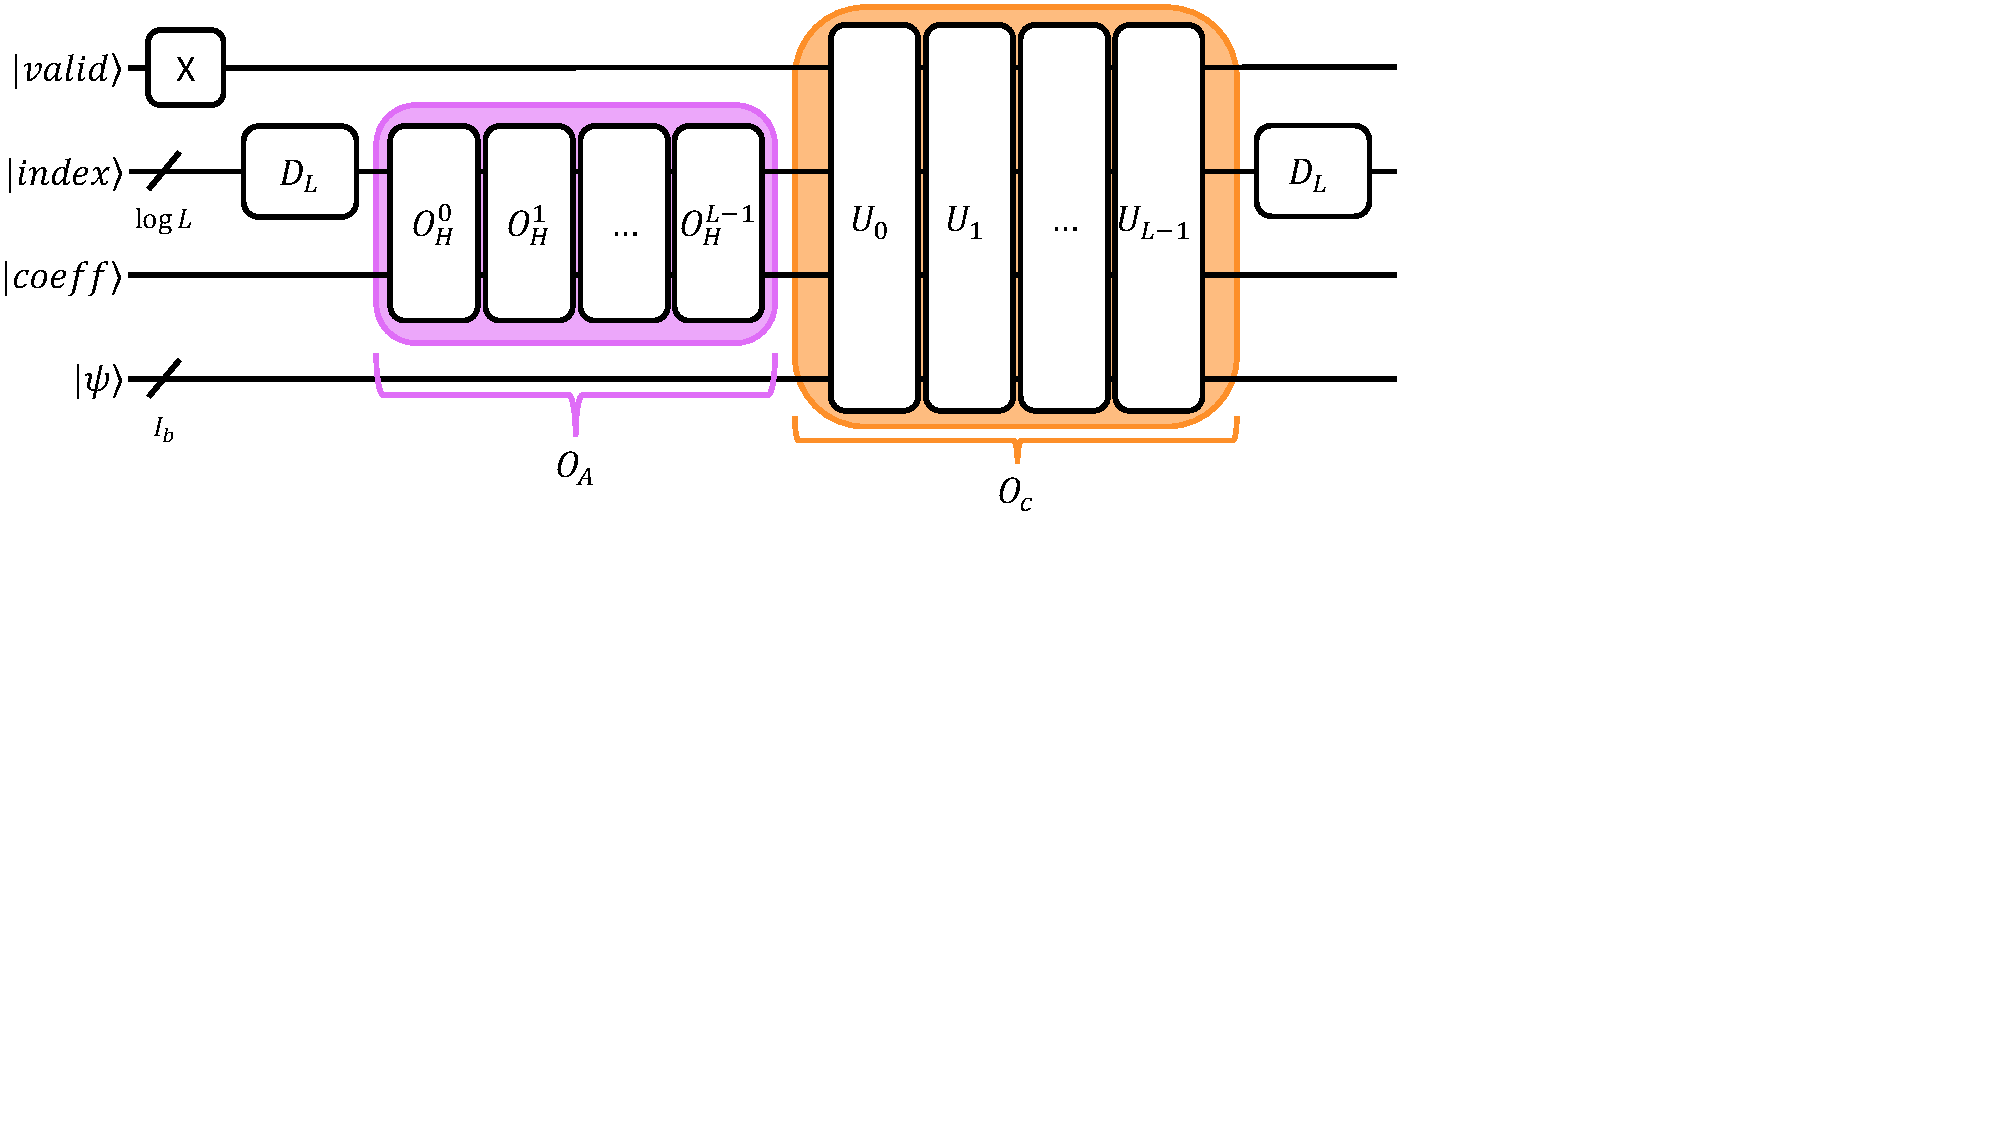
\includegraphics[width=12cm]{figures/liu-construction.pdf}
    \caption{
        \textbf{Sparse-Oracle Block-Encoding Circuit for Pairing Hamiltonians}
        A circuit diagram for the block-encoding described by Liu et. al \cite{liu2024efficient} is shown.
        The $O_A$ oracle is implemented by the series of $O_H^l$ operators (shaded in purple) which load the coefficients of the $l^{th}$ term.
        The $O_c$ oracle is implemented by the series of $U_l$ operators (shaded in orange) which apply the $l^{th}$ term onto the state.
        The $D_L$ oracle represents the diffusion operator (Eq. \ref{eq:diffusion-had}) acting on $L$ terms where $L$ is raised to the nearest power of two.
        The unitary $U_H = D_L O_c O_A D_L$ implements a block-encoding of the pairing Hamiltonian (Eq. \ref{eq:pairing-ham}) assuming the validation qubit ($\ket{\text{valid}}$) is initialized in the $\ket{1}$ state.
        The rescaling factor of this block encoding is given by $\lambda = L \max_{ij} {|h_{ij}|}$.
    }
    \label{fig:liu-construction}
\end{figure}

The structure of the circuits to block-encoding the pairing Hamiltonian is given in Figure \ref{fig:liu-construction}.
The sequence of $O_H^l$ unitaries implement the $O_A$ oracle and the sequence of $U_l$ unitaries implement the $O_c$ oracle.

\begin{figure}[h]
    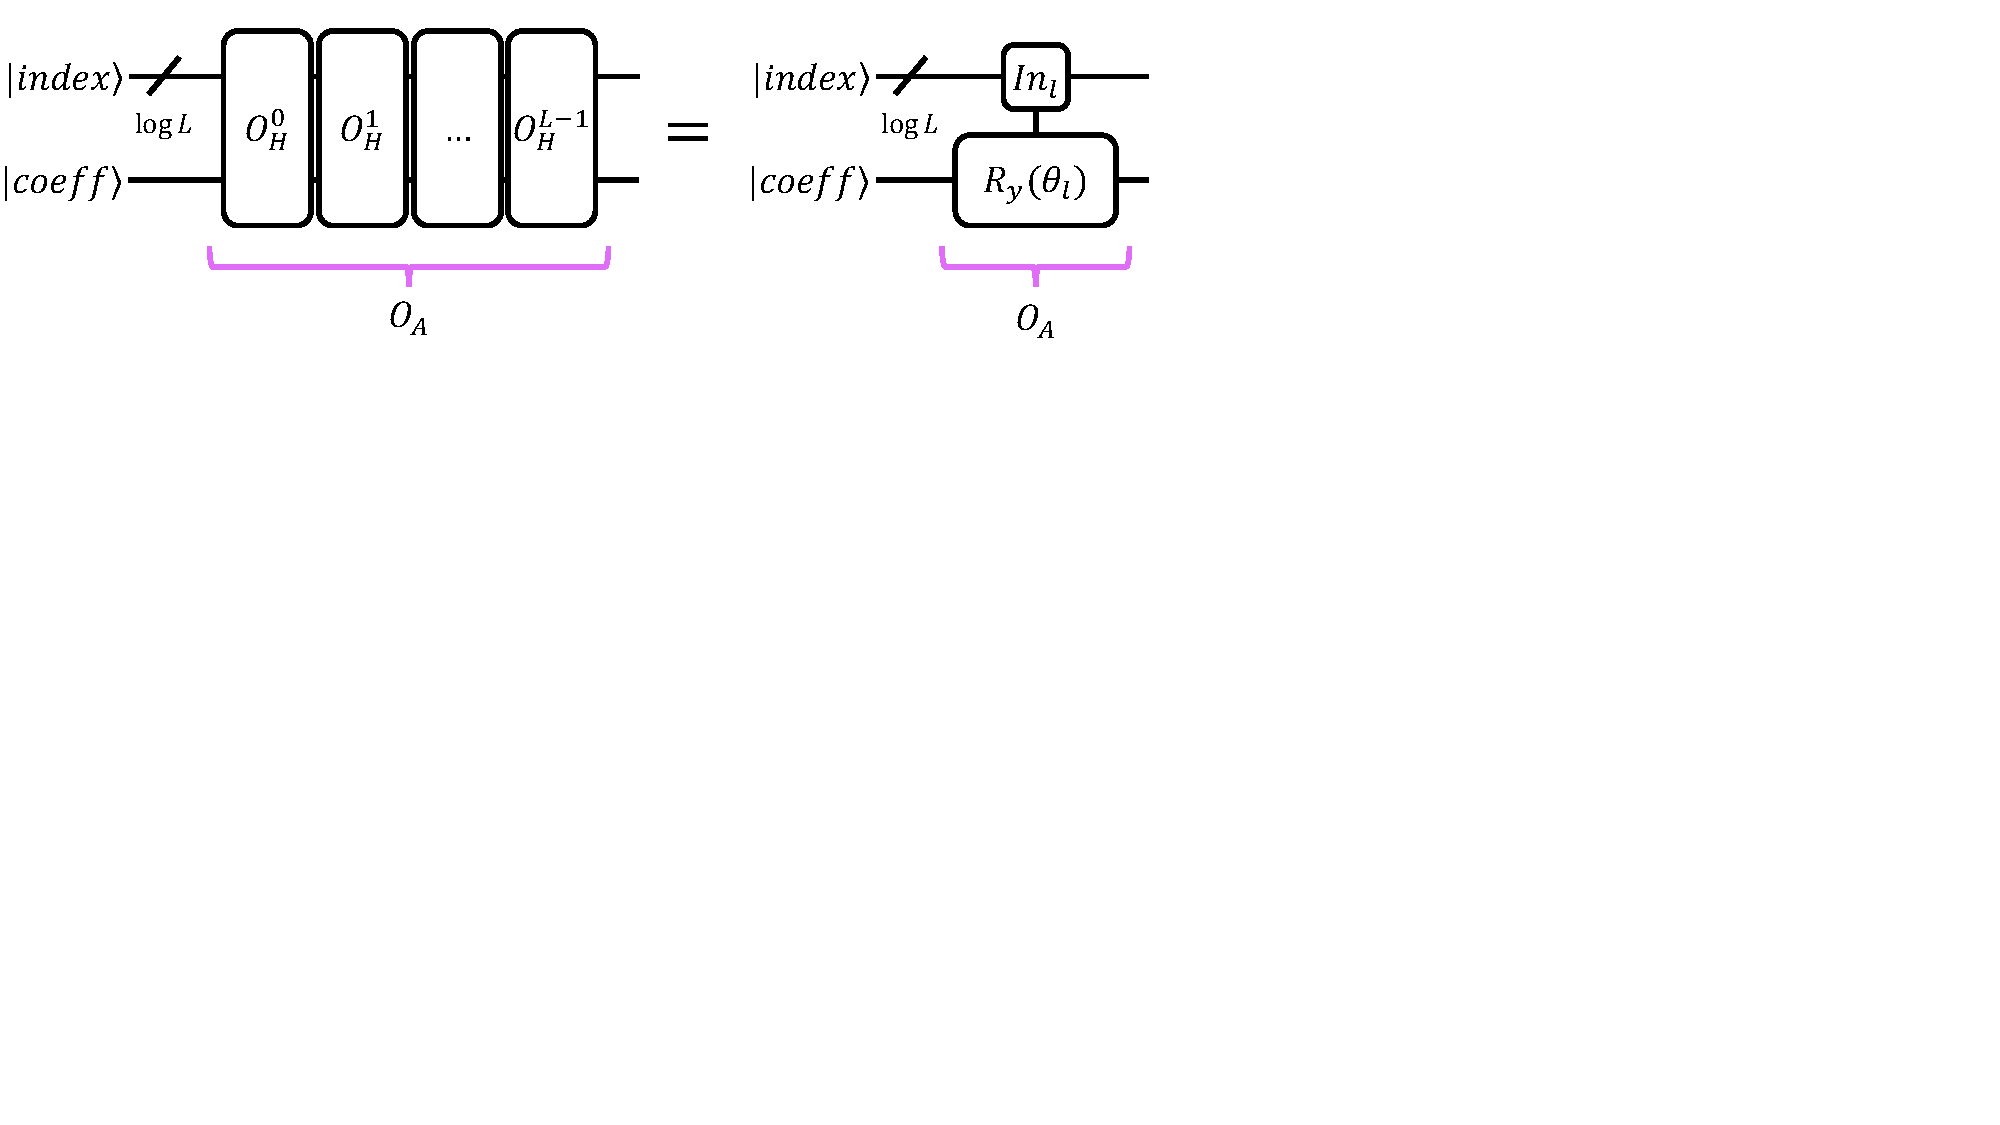
\includegraphics[width=12cm]{figures/liu-O_A.pdf}
    \caption{
        \textbf{$O_A$ Circuit for Pairing Hamiltonians}
        A circuit diagram for the $O_A$ oracle described by Liu et. al \cite{liu2024efficient}.
        Each unitary in the subfigure on the left performs an $R_y$ rotation on the coefficient qubit, controlled on the index register being in the computational basis state $\ket{l}$.
        This sequence of controlled rotations is referred to as a set of uniformly controlled rotations which is depicted by the subfigure on the right.
        Further discussion of compiling uniformly controlled rotations is given in Appendix \ref{sec:multiplexed-rotations}.
    }
    \label{fig:liu-O_A}
\end{figure}

Following Eq. \ref{eq:value-oracle}, the $O_A$ oracle rotates an ancilla qubit ($\ket{\text{coeff}}$ in Figure \ref{fig:liu-construction}) proportionally to the coefficient of the $l^\text{th}$ term when the index register ($\ket{\text{index}}$) is in the computational basis state $\ket{l}$.
This can be achieved by an $R_y$ rotation:
\begin{equation}
    \begin{split}
        & R_y (\theta_l) \ket{0}_\text{coeff} = h_{ij} \ket{0}_\text{coeff} + \sqrt{1 - |h_{ij}|^2} \ket{1}_\text{coeff} \\
        & \theta_l = 2 \cos^{-1}{(h_{ij})}
    \end{split}
\end{equation}
where the rotation is controlled on the index register being in the $l^\text{th}$ computational basis state.

This sequence of rotations controlled on the basis states of the index register is sometimes referred to as a set of uniformly controlled rotations.
When the axis of the rotations is the same for each rotation (as is the case here), the decomposition given by Möttönen et. al \cite{mottonen2004transformation} can be applied.
Under this construction, the $O_A$ oracle can be implemented using $L$ uncontrolled rotations.
A further discussion of this compilation is given in Appendix \ref{sec:multiplexed-rotations}.

The $O_c$ oracle is constructed by the unitaries denoted as $U_0 \dots U_{L - 1}$ in Figure \ref{fig:liu-construction}.
Each unitary $U_l$ is controlled on the index register being in the computational basis state $\ket{l}$.
This series of controlled operations can again be described as a set of uniformly controlled operations where each operation being applied is constructed to apply a block-encoding of the $l^\text{th}$ term in the Hamiltonian onto the system register.

\begin{figure}[h]
    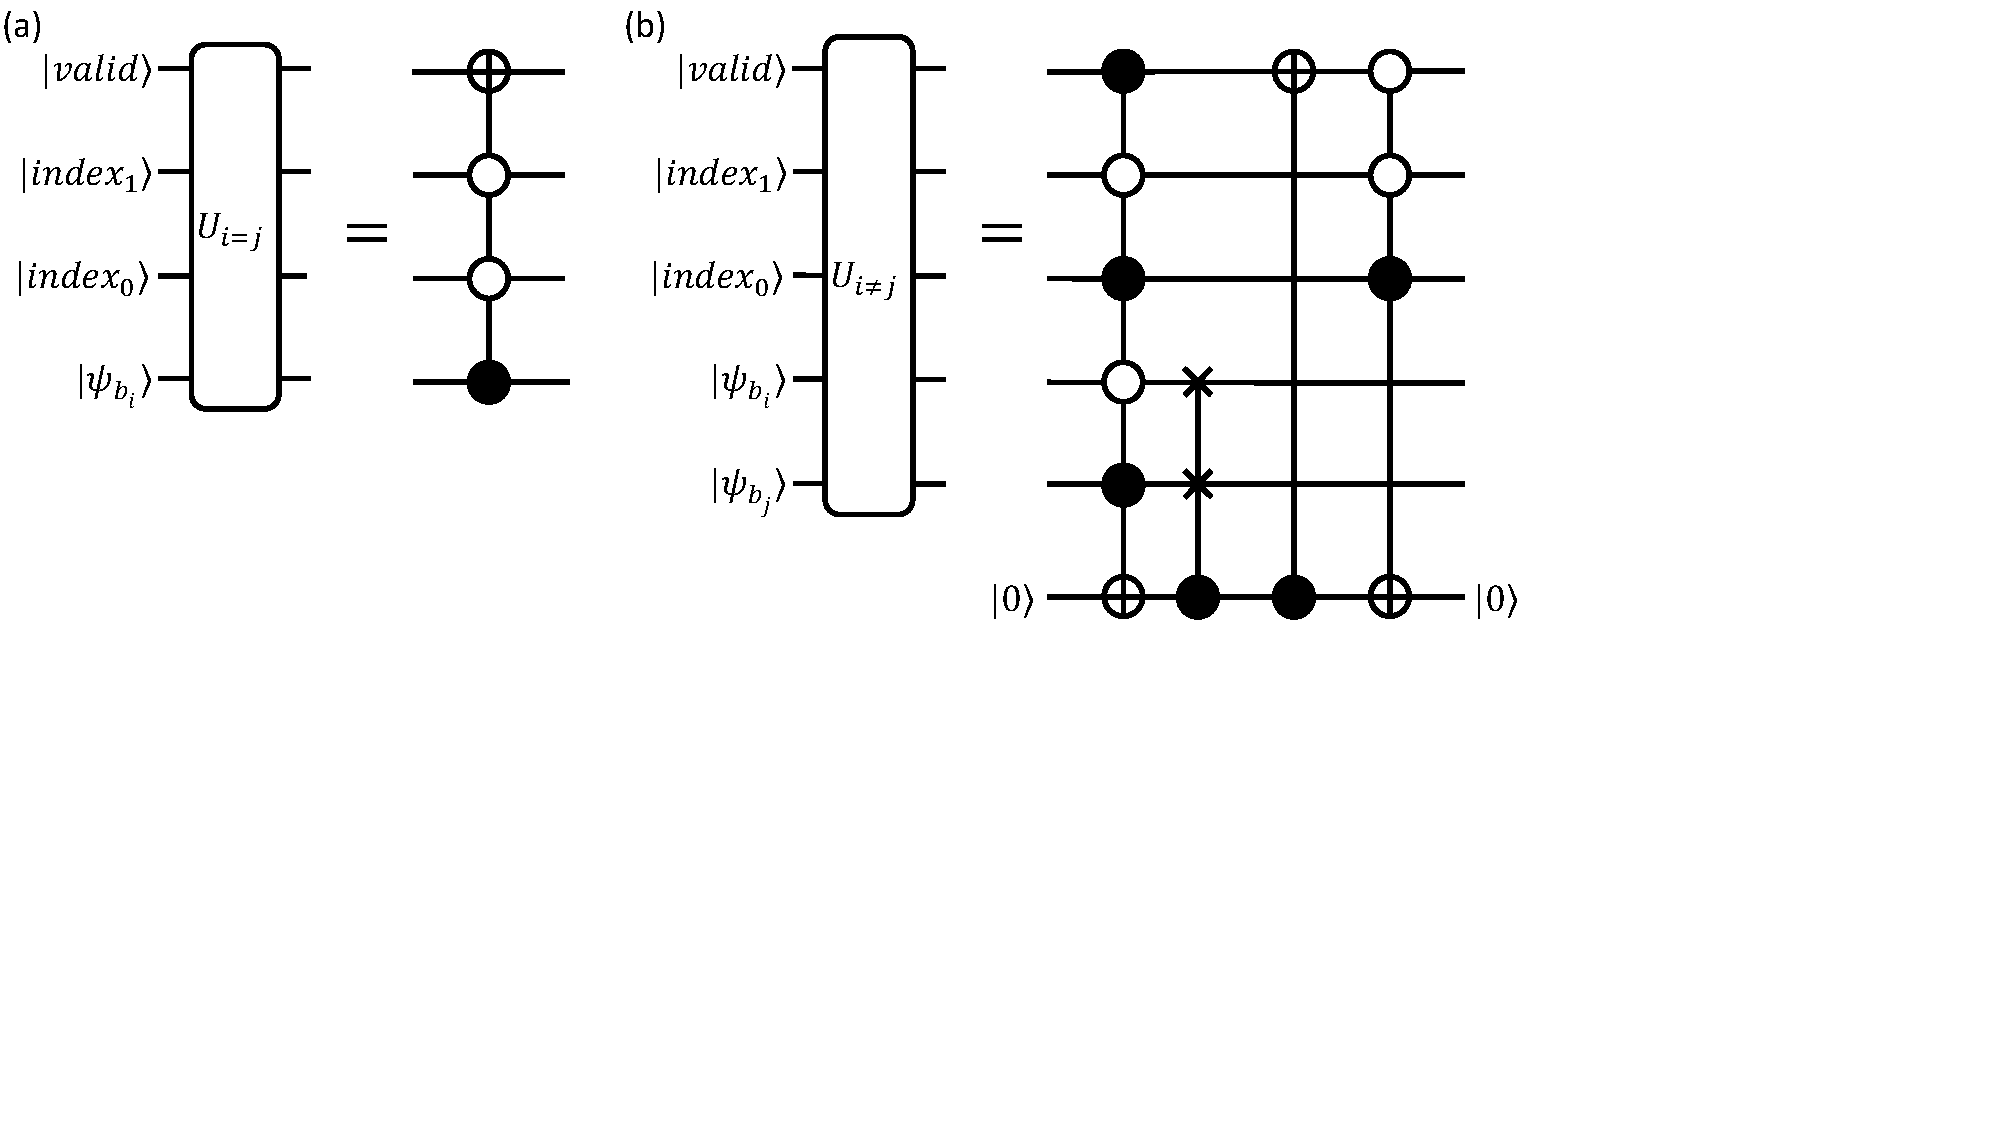
\includegraphics[width=12cm]{figures/liu-O_c.pdf}
    \caption{
        \textbf{$O_c$ Circuit Components for Pairing Hamiltonians}
        A circuit diagram for the unitaries comprising the $O_c$ oracle described by Liu et. al \cite{liu2024efficient} are shown.
        The circuit in subfigure a shows the unitary $U_{i = j}$ which applies a block-encoding of the operator $b_i^\dagger b_i$ when the index register is in the computational basis state $\ket{0}$. 
        The circuit in subfigure a shows the unitary $U_{i \neq j}$ which applies a block-encoding of the operator $b_i^\dagger b_j$ when the index register is in the computational basis state $\ket{1}$. 
    }
    \label{fig:liu-O_c}
\end{figure}

Liu et. al give constructions for applying the terms in the pairing Hamiltonian onto the system under the two cases $i = j$ and $i \neq j$.
In their construction, the validation qubit is initialized in the $\ket{1}$ state and is used to block-encode the individual terms in the Hamiltonian.

When the index for the ladder operators in Eq. \ref{eq:pairing-ham} are the same ($i = j$), the operator $b_i^\dagger b_i$ should zero-out the quantum state when the $i^\text{th}$ mode is unoccupied and should leave the state unchanged when the mode is occupied. 
For these terms, the desired action on the validation qubit is to leave it unaltered when the mode is unoccupied and flip the state of the validation qubit to $\ket{0}$ when the mode is occupied.
This can be achieved by a Toffoli gate which is controlled on the $i^\text{th}$ mode being occupied and the index register being in the computational basis state $\ket{l}$.
An example of these operators is given in Figure 11 of \cite{liu2024efficient} and we give a reproduction in Figure \ref{fig:liu-O_c}a.

When the indices that the ladder operators act on are not the same ($i \neq j$), the operator $b_i^\dagger b_j$ should zero-out the quantum state unless both the $i^\text{th}$ mode is unoccupied \textit{and} the $j^\text{th}$ mode is occupied.
Otherwise, the system of the state would be zeroed-out which would be indicated by leaving the validation qubit unchanged (in the $\ket{1}$ state).
If these conditions are true, a swap gate can be applied to swap the occupations of the fermionic modes and the validation qubit should be flipped to the $\ket{0}$ state. 

To perform this action, an ancillae qubit can be used to store the logical-AND of the conditions on the validation qubit, the index register, and the occupation states of the fermionic modes.
We assume that this ancilla qubit begins in the $\ket{0}$ state and the intent will be to return it to the $\ket{0}$ state such that it can be reused on subsequent operations.
In this work, we refer to qubits that are only temporarily rotated outside of the $\ket{0}$ state as clean ancillae.
An example for a circuit to perform this operation is also given in Figure 11 of \cite{liu2024efficient} and we give a reproduction in Figure \ref{fig:liu-O_c}b.
We note that to properly uncompute the ancilla qubit and return it to the $\ket{0}$ state we include the controls on the index register.
These controls are not present in the constructions given by Liu et. al, but must be included to properly reset this ancilla qubit.
\ws{Determine if construction by Liu et. al is actually incorrect or just incorrect if you want to treat the ancilla qubit as a clean ancilla.}

The controls on the index register for each $U_l$ comprising the $O_c$ oracle ensure that only the $l^\text{th}$ term is applied when the computational basis state is in the $\ket{l}$ state.
These controls on the index register are present for each term and can be accounted for by the uniformly controlled operation structure discussed in more detail in Appendix \ref{sec:uniformly-controlled-operations}.



\subsection{Linear Combination of Unitaries}
\label{subsec:lcu}

Suppose we wish to generate a block-encoding of an operator that can be written as a linear combination of unitary operators:
\begin{equation}
    \label{eq:lcu}
    A = \sum_{l=0}^{L-1} \alpha_l U_l
\end{equation}
where $\alpha_l$ are real-valued coefficients and each $U_l$ is a unitary operator.
The restriction here on real-valued coefficients is simply to be clear about the cost of block-encoding this operator. 
If we wish to include terms with imaginary coefficients, we can absorb the imaginary phase into the operator: $i \alpha_l U_l = \alpha_l U_l^\prime$.
Likewise, a term with a complex coefficient can be treated as two distinct terms ($U_l$ and $U_l^\prime$) each with a real coefficient, though this increases the number of terms ($L$).
\ws{Question: when we decompose a state into a linear combination of other states we say we expand it in some basis. What is the wording for when we expand an operator in a basis of operators?}

Assuming that $A$ is sparse in this description - $L$ grows polynomially with $N_A$ - then the Sparse-Oracle framework generates a valid block-encoding of $A$ where the rescaling factor would be $\lambda = 2^{\lceil \log_2 L \rceil} \max_{l} |\alpha_l|$.
In this construction, $O_A$ would load the (rescaled) coefficients $\{\alpha_l\}$ and $O_c$ would apply the unitaries $\{U_l\}$ onto the system register controlled on the index register being in the computational basis states $\{\ket{l}\}$. 

However, an alternative framework proposed by Childs et. al \cite{childs2012hamiltonian} called Linear Combination of Unitaries (LCU) is \textit{specifically} designed for generating block-encodings of operators in the form of Eq. \ref{eq:lcu}. 
With two oracles, \textit{Prepare} and \textit{Select}, an LCU block-encoding can be defined as follows:
\begin{theorem}
    \label{th:lcu}
    Given a matrix $A$ defined by Eq. \ref{eq:lcu}, let the oracles \textbf{Prepare} and \textbf{Select} be defined by:
    \begin{equation}
        \label{eq:prep-state}
        \textbf{Prepare}\text{:} \ket{0^{\otimes \lceil \log_2 L \rceil}}_\text{index} \rightarrow \sum_{l=0}^{L-1} \sqrt{| \alpha_l | / \lambda} \ket{l}_\text{index}
    \end{equation}
    where $\lambda$ is given by $\lambda_\text{LCU}$ (defined below) and
    \begin{equation}
        \label{eq:select}
        \textbf{Select}\text{:} 
        \begin{cases} 
            \text{Apply $U_l$ on $\ket{\psi}$} & \text{when $\ket{\text{index}}$ is $\ket{l}$} \\
            \text{Undefined} & \text{Otherwise} \\
        \end{cases}
    \end{equation}
    where the \textbf{Select} oracle applies the unitary $U_l$ on the system register when the index register is in the computational basis state $\ket{l}$ and the action is not strictly defined for other states of the index register.

    Then a block-encoding for $A$ is given by:
    \begin{equation}
        \label{eq:lcu-be}
        U_A = (\textbf{Prepare}^\dagger) (\textbf{Select}) (\textbf{Prepare})
    \end{equation}
    with a rescaling factor of:
    \begin{equation}
        \lambda_\text{LCU} = \sum_{l=0}^{L-1} | \alpha_l |
    \end{equation}
\end{theorem}
A simple proof that $U_A$ block-encodes $A$ is given in Section 7.3 of Lin et. al \cite{lin2022lecture}.

The rescaling factor for an LCU block-encoding is given by the 1-norm of the coefficients in Eq. \ref{eq:lcu} and ensures that the corresponding $\bar{U}_l$ has spectral norm less than or equal to $1$.
A benefit of an LCU block-encoding over a Sparse-Oracle block-encoding is the smaller rescaling factor.
A simple proof that $\lambda_\text{LCU} \leq \lambda_\text{SO}$ is given in Appendix \ref{sec:proof-of-rescaling-factors}.

\subsubsection{Implementing \textbf{Prepare}}

The \textit{Prepare} oracle serves a similar role to the $O_A$ oracle in that it loads the coefficients or the values of the matrix elements onto the quantum computer.
The action of the \textit{Prepare} oracle defined by Eq. \ref{eq:prep-state} is to map the all-zero state of an ancilla register to a particular superposition state where the squared amplitudes of the computational basis states are weighted to encode the coefficients of the terms in the operator.
We refer to this ancilla register as the \textit{index register} as the computational basis states of this register, $\ket{l}$, index the $L$ terms in A.

The matrix representation for a valid implementation of the \textit{Prepare} oracle in the computational basis is given by:
\begin{equation}
    \text{Prepare} = \begin{bmatrix}
        \sqrt{|\alpha_0| / \lambda_\text{LCU}} & * & ... & * \\
        \sqrt{|\alpha_1| / \lambda_\text{LCU}} & * & ... & * \\
        \vdots & \vdots & \ddots & \vdots \\
        \sqrt{|\alpha_{L-1} |/ \lambda_\text{LCU}} & * & ... & * \\
    \end{bmatrix}
\end{equation}
From this definition, it is clear that there are infinitely many unitaries that implement the $\textit{Prepare}$ oracle since only the first column of the operator is fixed.

For operators that have structure among the coefficients of the terms, implementations of $\textit{Prepare}$ can be constructed that leverage this structure to reduce the time cost of implementing the oracle.
In certain cases, this can drastically reduce the cost such as is done for the Fermi-Hubbard model in \cite{babbush2018encoding} where there are only two unique coefficients in the LCU.

When a certain structure is not present, the Grover-Rudolph algorithm \cite{grover2002creating} gives a formulaic routine to generate quantum circuits that implement the $\textit{Prepare}$ oracle.
Although the cost of implementing Grover-Rudolph scales exponentially with the number of qubits in the register it acts upon, the size of the index register is logarithmic in the number of terms in the operator being block-encoded.
Therefore, the cost of Grover-Rudolph will be linear in $L$.
If A is \textit{sparse} - $L$ grows polynomially with respect to $N_A$ - then the cost of Grover-Rudolph will be polynomial with respect to $N_A$.  

\subsubsection{Implementing \textbf{Select}}

Similar to the $O_c$ oracle, the desired action of the \textit{Select} oracle is to apply the unitary $U_l$ onto the system register \textit{controlled} on the index regsiter being in the state $\ket{l}$ (Eq. \ref{eq:select}).
Since the action of the \textit{Select} oracle is undefined when the computational basis states of the index register is greater than $L - 1$, there are also infinitely many valid quantum circuits for implementing \textit{Select}.

\begin{figure}[h]
    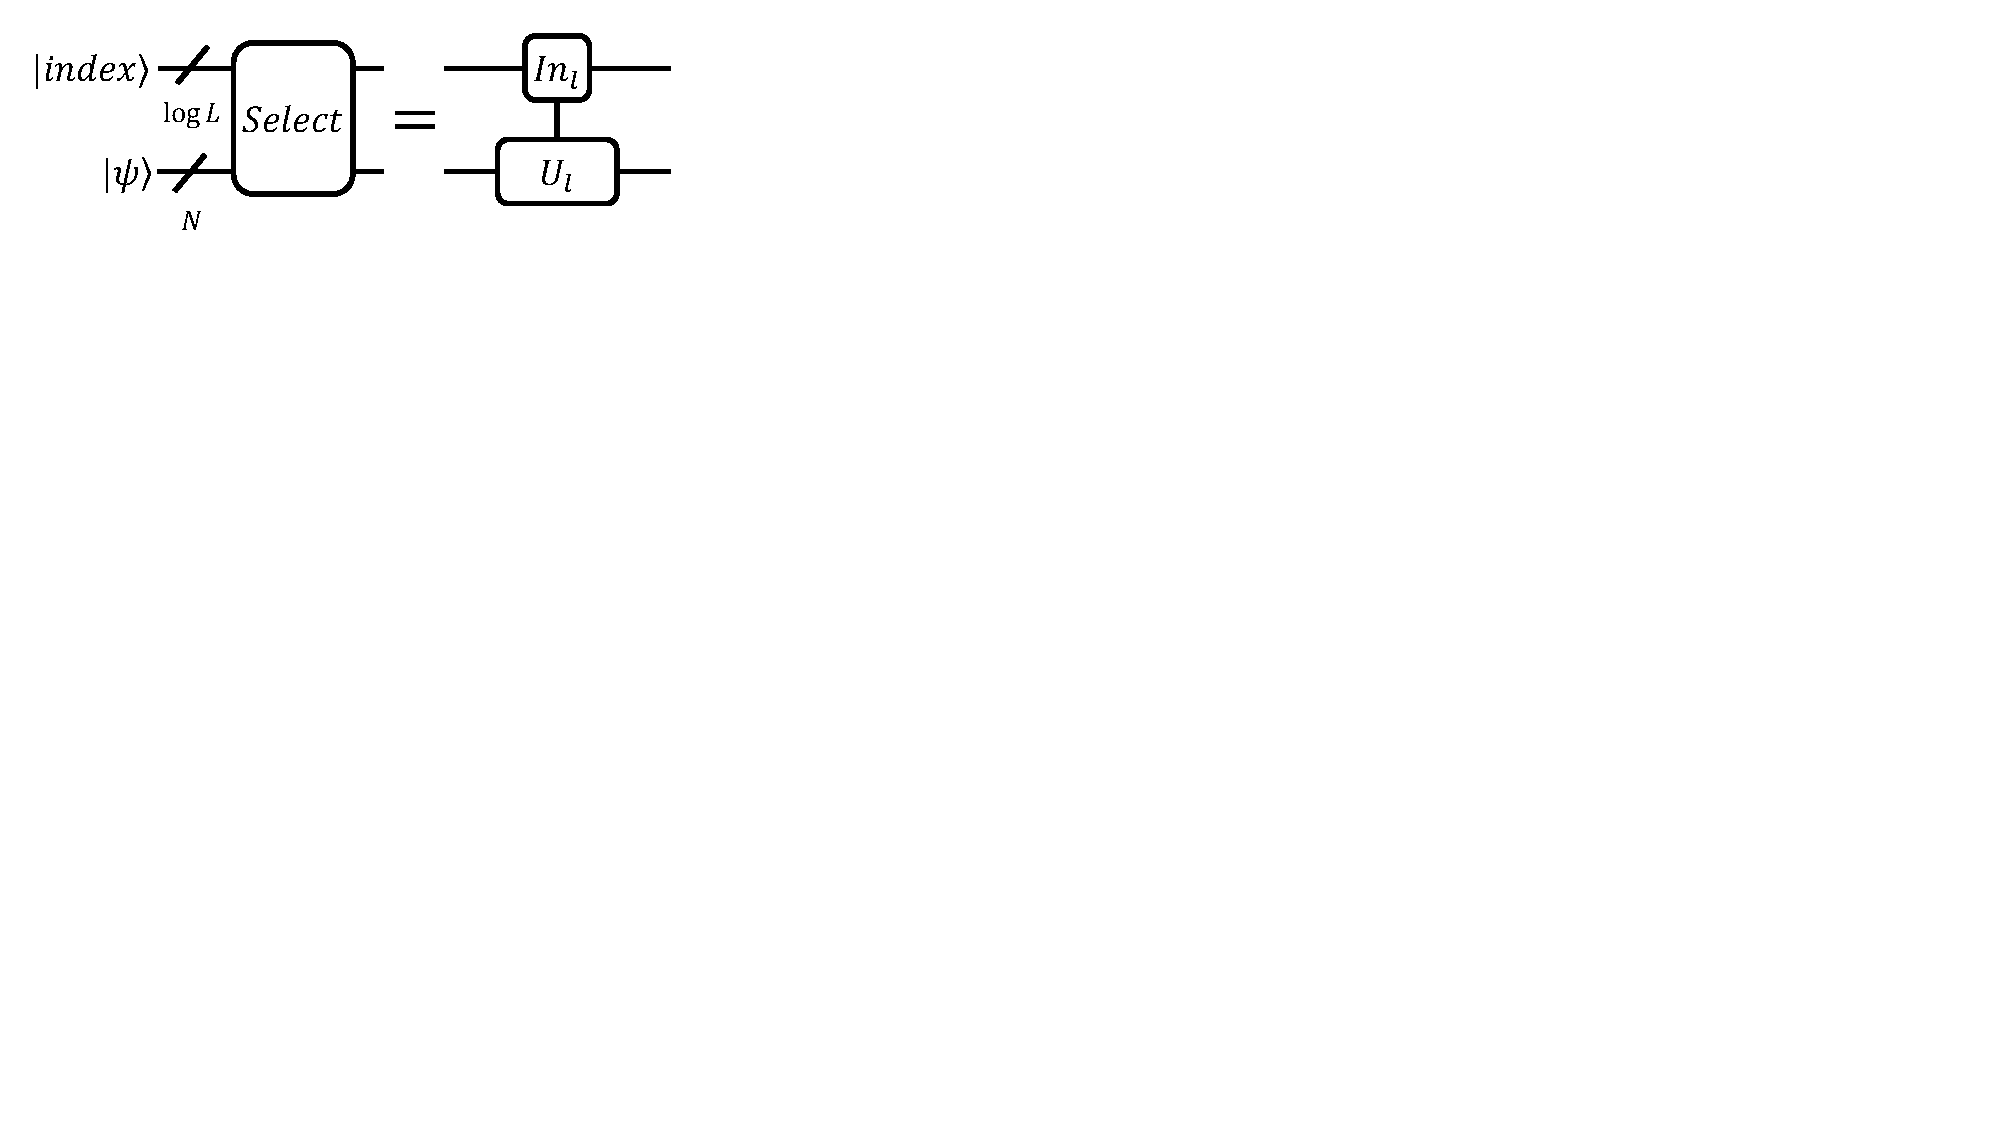
\includegraphics[width=6cm]{figures/select-lcu.pdf}
    \caption{
        \textbf{LCU \textit{Select} Oracle}
        A circuit diagram for the \textit{Select} oracle in LCU is shown.
        This is a naive implementation where no structure in the operator is assumed.
        The \textit{Select} oracle applies the $l^\text{th}$ unitary in the LCU (Eq. \ref{eq:lcu}) onto the system when the index register is in the computational basis state $\ket{l}$
        This can be achieved using a set of uniformly controlled operations (right subfigure).
    }
    \label{fig:unstructured-select}
\end{figure}

If structure in the problem is present, the \textit{Select} oracle can be implemented to leverage that structure as is done in \cite{babbush2018encoding}.
Without any assumptions on the structure in $A$, the \textit{Select} oracle can be implemented by the operator:
\begin{equation}
    \label{eq:select-naive}
    \text{Select} = \sum_{l=0}^{L-1} \ket{l}\bra{l} \otimes U_l
\end{equation}
Similar to the $O_A$ and $O_c$ oracles, the \textit{Select} oracle serially controls upon the computational basis states of the index register and this control structure can be grouped together as a uniformly controlled operation which is discussd in more detail in Appendix \ref{sec:uniformly-controlled-operations}.
This is shown in Figure \ref{fig:unstructured-select}.

As a quick aside, if the implementation of the \textit{Select} oracle is self-inverse, then the LCU block-encoding is also self-inverse.
This structure makes LCU block-encodings particularly well-suited for being applied in algorithms based on Qubitization \cite{low2019hamiltonian}.
Using the construction for \textit{Select} in Eq. \ref{eq:select-naive}, the implementation will be self-inverse if the unitaries themselves are self-inverse.
As an example, this is the case for when the operator $A$ is decomposed in the Pauli basis as the Paulis are self-inverse. 

\subsection{Linear Combination of Operators}
\label{subsec:unification}

LCU block-encodings provide better rescaling factors, yet there are clearly parallels between the $O_A$ oracle and the \textit{Prepare} oracle, as well as the $O_c$ oracle and the \textit{Select} oracle.
Therefore one might ask if we can construct LCU-style block-encodings for a linear combination of \textit{operators} under the assumption that we have access to block-encodings of each operator:
\begin{equation}
    \label{eq:lco}
    A = \sum_{l=0}^{L-1} \alpha_l O_l
\end{equation}
where the $O_l$ are operators and we again restrict the coefficients $\alpha_l$ to be real-valued for simplicity, yet the same strategies to apply operators with imaginary or complex-valued coefficients used for an LCU can be applied here.
% We also restrict the spectral norms of the operators to satisfy $|\bar{O}_l| \leq 1$ for simplicity and note that we can rescale any operator to satisfy this condition and let the rescaling factor be absorbed by the corresponding coefficient.
% However, we note that extra care must be taken when absorbing these rescaling factors such that the rescaling of the linear combination is consistent across all terms.

Another way to frame this is creating an LCU block-encoding where the unitary operators themselves are block-encodings of operators which is described in Section 4.3 of Gilyén et. al \cite{gilyen2019quantum} and noted by Jennings et. al \cite{jennings2023efficient}.
We will refer to this method of block-encoding as an LCO block-encoding (Linear Combination of Operators).
As noted by Jennings et. al \cite{jennings2023efficient} it may be enlightening to consider an LCU block-encoding as a apecial case of an LCO block-encoding wherein the operators in the linear combination are all unitary.

\begin{theorem}
    \label{th:lco}
    Given a matrix $A$ defined by Eq. \ref{eq:lco} and unitary operators $U_l$ that each block-encode the operators $O_l$:
    \begin{equation}
        \label{eq:applying-operator}
        U_l \ket{\psi}\ket{0}_\text{anc} = \bar{O}_l \ket{\psi} \ket{0}_\text{anc} + \beta_{\psi, l} \ket{\perp}
    \end{equation}
    with rescaling factors $\lambda_l$ such that $\lambda_l \bar{O}_l = O_l$.
    
    Define the \textbf{Prepare} oralce by:
    \begin{equation}
        \label{eq:prep-lco}
        \textbf{Prepare}\text{:} \ket{0^{\otimes \lceil \log_2 L \rceil}}_\text{index} \rightarrow \sum_{l=0}^{L-1} \sqrt{| \bar{\alpha}_l | / \lambda} \ket{l}_\text{index}
    \end{equation}
    where $\bar{\alpha_l}$ is given by:
    \begin{equation}
        \label{eq:rescaled-coeffs}
        \bar{\alpha_l} = \frac{\alpha_l \lambda_l}{\max_{l^\prime}{\lambda_{l^\prime}}}
    \end{equation}
    and $\lambda$ is given by:
    \begin{equation}
        \lambda = \sum_{l=0}^{L-1} \bar{\alpha_l}
    \end{equation}

    Define the \textbf{Select} oracle by:
    \begin{equation}
        \label{eq:select-conditions-lco}
        \textbf{Select}\text{:} 
        \begin{cases} 
            \text{Apply $U_l$ on $\ket{\psi}\ket{0}_\text{anc}$} & \text{when $\ket{\text{index}}$ is $\ket{l}$} \\
            \text{Undefined} & \text{Otherwise} \\
        \end{cases}
    \end{equation}
    where the \textbf{Select} oracle applies a block-encoding of $O_l$ on the system register using an additional ancilla register when the index register is in the computational basis state $\ket{l}$ and the action is not strictly defined for other states of the index register.

    Then a block-encoding for $A$ is given by:
    \begin{equation}
        \label{eq:lco-be}
        U_A = (\textbf{Prepare}^\dagger) (\textbf{Select}) (\textbf{Prepare})
    \end{equation}
    with a rescaling factor of:
    \begin{equation}
        \lambda_\text{LCO} = \big(\max_{l}{\lambda_l}\big) \sum_{l=0}^{L-1} | \bar{\alpha}_l | = \sum_{l=0}^{L-1} |\alpha_l \lambda_l|
    \end{equation}
\end{theorem}
The proof that $U_A$ block-encodes $A$ follows from the same proof for LCU block-encodings given by Lin et. al \cite{lin2022lecture}.

To motivate that this rescaling factor is more favorable than a Sparse-Oracle block-encoding, consider the case of the pairing Hamiltonian.
Using the construction given by Liu et. al, the rescaling factor for $H$ is given by:
\begin{equation}
    \lambda_\text{SO}^H = 2^{\lceil \log_2 L \rceil} \max_{ij} |h_{ij}|
\end{equation}
Since each operator in Eq. \ref{eq:pairing-ham} has a spectral norm of $1$, then the rescaling for an LCO block-encoding is simply given by:
\begin{equation}
    \lambda_\text{LCO}^H = \sum_{ij} |h_{ij}|
\end{equation}
and the proof that $\lambda_\text{LCO}^H \leq \lambda_\text{SO}^H$ follows directly from the proof given in Appendix \ref{sec:proof-of-rescaling-factors}.

Implementing the LCO \textit{Prepare} and \textit{Select} oracles can be done similarly to the LCU oracles.
The \textit{Prepare} oracle follows directly from LCU using the rescaled coefficients $\{\bar{\alpha}_l\}$ defined by Eq. \ref{eq:rescaled-coeffs}. 
If structure among the coefficients is present, then this structure can be exploited. 
If no structure exists, then the Grover-Rudolph algorithm can be applied.

The construction for \textit{Select} can again leverage the problem structure if such a structure exists, or it can be generated using uniformly controlled operations following:
\begin{equation}
    \label{eq:select-lco}
    \text{Select} = \sum_{l=0}^{L-1} \ket{l}\bra{l} \otimes U_l
\end{equation}
where the block-encodings for the operators $O_l$ can be constructed using any of the frameworks discussed here.
\section{Ladder Operator Block-Encoding (LOBE)}
\label{sec:lobe}

The block-encodings presented in this work builds off of the constructions of \cite{camps2024explicit} and \cite{liu2024efficient} to provide a more general block-encoding of Hamiltonians described in the form of Eq. \ref{eq:lclo}.
Explicity, the construction presented in this work allows for the terms in the Hamiltonian to be any arbitrary product of ladder operators acting on fermions, antifermions, and bosons.
Additionally, we make use of the observations presented in Subsection \ref{subsec:lco} to provide block-encodings of the same structure as an LCU which have reduced rescaling factors.
This also extends LCU block-encodings to the non-unitary operators used in this work and may provide a framework for constructing block-encodings of linear combinations of other non-unitary operators.

\begin{figure}
    \centering
    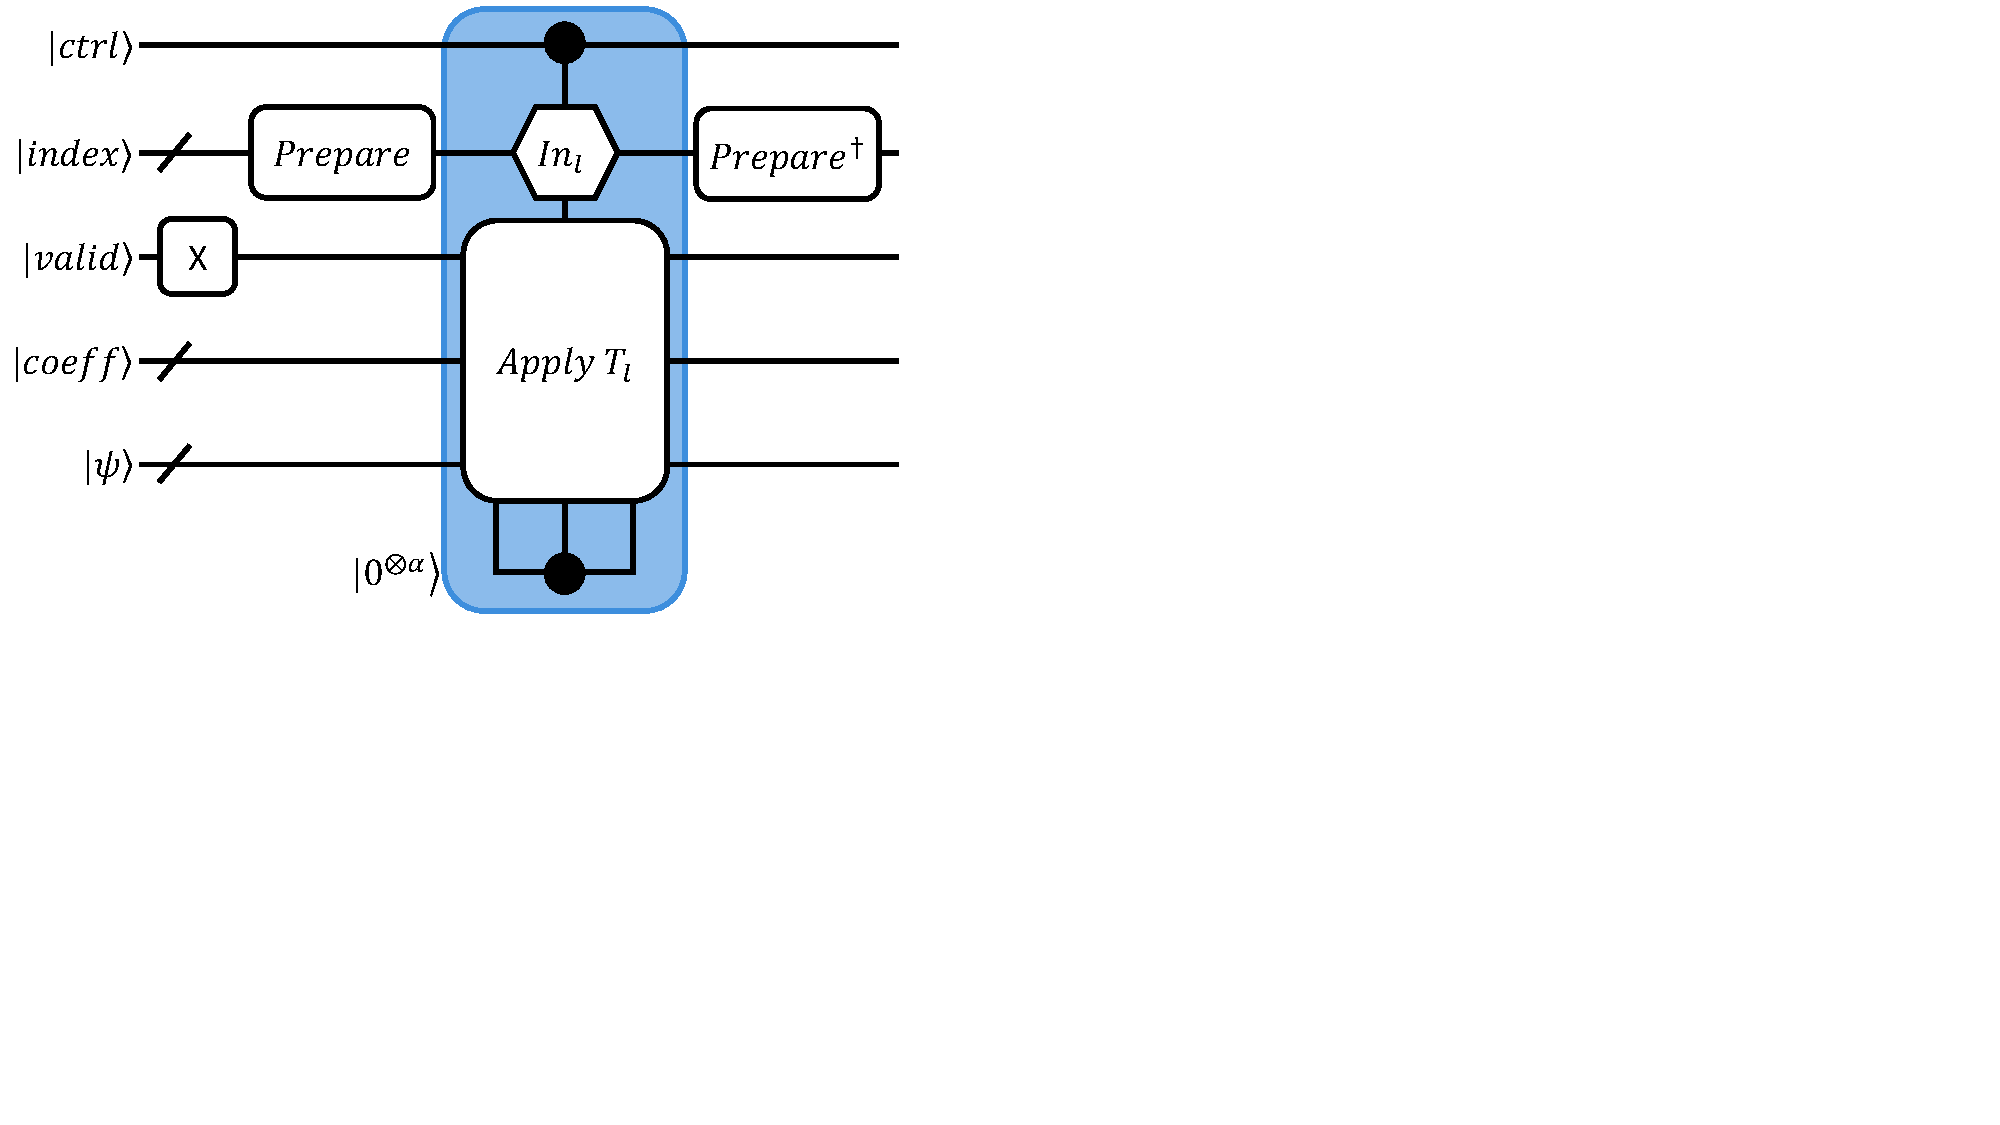
\includegraphics[width=8cm]{figures/lobe.pdf}
    \caption{
        \textbf{Ladder Operator Block-Encoding (LOBE)}
        A circuit diagram for a \textit{controlled} application of LOBE is shown. 
        The Pauli-X gate on the validation qubit depicts that the validation qubit begins in the $\ket{1}$ state and this operation is not repeated on subsequent calls to the block-encoding.
        The block-encoding is structured in the same way as an LCU block-encoding where a \textit{Prepare} oracle is applied on the index register, followed by an application of a \textit{Select} oracle (shaded in blue), and then finishes by uncomputing the index register using $\textit{Prepare}^\dagger$.
        Throughout this work, hexagons in circuit diagrams will represent multiplexors over the register on which they are applied.
        The multiplexor depicted with $\textit{In}_l$ in this diagram creates a coherent for-loop over the computational basis states of the index register and is constructed as shown in Figure 7 of \cite{babbush2018encoding}.
        The bottom register denoted $\ket{0^{\otimes Q_\alpha}}$ depicts a clean ancillae register which is promised to have qubits beginning and ending in the $\ket{0}$ state.
    }
    \label{fig:lobe}
\end{figure}

In Figure \ref{fig:lobe}, we define the LOBE circuit in terms of generic oracles.
The LOBE circuit is structured similarly to an LCU circuit in that it involves sequential application of a $\textit{Prepare}$ oracle, a $\textit{Select}$ oracle, and then uncomputing the $\textit{Prepare}$ oracle using the daggered circuit.

There are numerous space-time tradeoffs that one can make to either reduce the number of ancillae qubits at the cost of more gates or vice versa.
In this work, we opt for compilations that minimize the number of non-Clifford operations at the expense of more ancillae qubits.

Since the most costly operations to perform are those that will require preparation of magic states (non-Clifford operations) \ws{Is this only true for surface code?}, the analytical gate counts will be computed in terms of the following non-Clifford operations: (arbitrary rotations, left elbows, right elbows).
For ease, we will express these gate counts as an ordered tuple:
\begin{equation}
    \label{eq:gate-counts}
    C = (N_{\textit{rot}}, N_{\textit{left}}, N_{\textit{right}})
\end{equation}
where left and right elbows are defined by \cite{babbush2018encoding}.

A single left-elbow produced from 2 controls will require 1 clean ancilla qubit and 4 T gates. 
A corresponding right-elbow will require a measurement and a classically conditioned Clifford operation.
As the exact cost of a right elbow will likely be highly dependent on the physical architecture and quantum error-correction scheme, it will be counted independently.
A left-elbow with $N$ controls producing one ancilla qubit storing the quantum boolean can be decomposed into elbows using only 2 controls each, using $N-1$ total ancillae (including the output boolean) with the following cost:
\begin{equation}
    \label{eq:N-ctrl-elbow}
    C_{N-ctrl-elbow} = (0, N-1, N-2)
\end{equation}

Additionally, arbitrary rotations are typically decomposed into non-Clifford operations via one of several methods \cite{ross2014optimal, bocharov2015efficient} \ws{cite addition with phase gradient states}.
The cost of these decompositions is dependent upon the desired rotation angle and the required precision on the angle of the rotation.
For this reason, we will leave these costs in terms of rotations and elbows instead of decomposing them further into T gates.

\subsection{Qubit Registers}
\label{subsec:registers}

The LOBE circuit makes use of 5 qubit registers: $\ket{\textit{index}}$, $\ket{\textit{valid}}$, $\ket{\textit{coeff}}$, $\ket{\psi}$, and $\ket{0^{\otimes Q_\alpha}}$.
This disregards the control qubit ($\ket{\textit{ctrl}}$) in Figure \ref{fig:lobe} as it is not required for applying an uncontrolled block-encoding.

The register denoted $\ket{\textit{index}}$ is referred to as the index register and is used to index the terms in the Hamiltonian as is done in LCU constructions. 
The integer representations of the computational basis states of the index register corresponds to the indices $l$ in Eq. \ref{eq:lclo}. 
The minimum number of qubits required for the index register is given by:
\begin{equation}
    Q_{\textit{index}} = \lceil \log_2{L} \rceil
\end{equation}

The register denoted $\ket{\textit{valid}}$ consists of a single qubit and is referred to as the validation qubit.
It serves the same purpose as in \cite{liu2024efficient} which is to denote whether or not the term at the current index ($T_l$) should be applied onto the system and if it will annihilate the quantum state.
Suppose the term $T_l$ will annihilate the state based on the occupation of the fermionic and antifermionic modes. 
In that case, the validation qubit remains in the $\ket{1}$ state such that that branch of the wavefunction remains outside the encoded subspace of the block-encoding.
This action on the validation qubit will be described in more detail in Subsection \ref{subsec:select}.
If the term will not annihilate the state, then the validation qubit gets flipped to the $\ket{0}$ state for the term $T_l$.
The validation qubit is initialized in the $\ket{1}$ state which can either be assumed or implemented via a single $X$ gate applied to the $\ket{\textit{valid}}$ qubit once it is initialized.
The single $X$ gate in Figure \ref{fig:lobe} depicts this initialization and is \textit{not} repeated on subsequent applications of the block-encoding.
\ws{Still need to explicitly verify this}

The register denoted $\ket{\textit{coeff}}$ is referred to as the coefficient register and is used to store the coefficients associated with the bosonic ladder operators in term $T_l$. 
% The number of qubits required for the bosonic coefficients is $A$ which is the maximum number of bosonic operators acting within a single term.
If we let $M$ denote the maximum number of bosonic modes with operators acting on them within a single term, then the minimum number of qubits in the coefficient register is given by:
\begin{equation}
    Q_{\textit{coeff}} = M 
\end{equation} 
% If $USP$ is used for preparation of the index register, then an additional qubit is required.
One additional qubit may be required to apply the $\alpha_l$ coefficient depending on the \textit{Prepare} oracle that is used.
% These coefficients include the coefficients associated with the bosonic ladder operators and can also include the coefficients of the terms in the linear combination ($\alpha_l$) depending on the \textit{Prepare} oracle that is used.

The register denoted $\ket{\psi}$ is referred to as the system register and is used to encode the state of the system.
This register can be broken up into three subsequent registers: the fermionic system $\ket{\psi_b}$, the antifermionic system ($\ket{\psi_d}$), and the bosonic system ($\ket{\psi_a}$).
% The encoding studied in this work is outlined in more detail in Subsection \ref{subsec:encoding}.
Using the qubit-efficient encoding described in Subsection \ref{subsec:encoding}, the minimum number of qubits required for the system registers is given by:
\begin{equation}
    \begin{split}
        &Q_{\psi_b} = I \\
        &Q_{\psi_d} = I \\
        &Q_{\psi_a} = I \lceil \log_2{(\Omega + 1)} \rceil \\
        &Q_{\psi} = Q_{\psi_b} + Q_{\psi_d} + Q_{\psi_a} = 2I + I\lceil \log_2{(\Omega + 1)} \rceil
    \end{split}
\end{equation} 

Finally, the register denoted $\ket{0^{\otimes Q_\alpha}}$ is referred to as the clean ancillae register where $Q_\alpha$ will be used to refer to the number of qubits in this register.
This register includes ancillae qubits that are promised to begin in the $\ket{0}$ state and are returned to this state at the end of the block-encoding circuit.
These temporary, clean ancillae are allocated and deallocated as the block-encoding circuit proceeds.
The maximum number of clean ancillae required is dependent upon the exact compilation methods for both \textit{Prepare} and \textit{Select}.

\subsection{Rescaling of Coefficients Due to Bosonic Terms}
\label{subsec:rescaling}

The inclusion of bosonic ladder operators in our models requires rescaling the coefficients of our Hamiltonian such that they are always normalized and appropriately weighted.
As shown in Eqs. \ref{eq:bosonic-creation} and \ref{eq:bosonic-annihilation}, bosonic ladder operators acquire a coefficient on the state that is proportional to the square-root of the occupation of the state.
From these definitions, it is clear that if we were to apply a block-encoding that contains bosonic ladder operators onto a quantum state, the output quantum state may not be normalized.

To remedy this, we can rescale the coefficients that are picked up by the operators such that the states are always normalized.
In the case of bosonic ladder operators, we can rescale Eqs. \ref{eq:bosonic-creation} and \ref{eq:bosonic-annihilation} by dividing by the square-root of the maximum allowable occupation number plus one such that any coefficient acquired is $< 1$:
\begin{equation}
    \label{eq:bosonic-ops-altered}
    \begin{split}
        \Tilde{a}_i^\dagger \ket{n_{a_i}} &= \sqrt{\frac{n_{a_i} + 1}{\Omega + 1}} \ket{n_{a_i} + 1} \hspace{1em} when \ket{n_{a_i}} \neq \ket{\Omega} \\
        \Tilde{a}_i  \ket{n_{a_i}} &= \sqrt{\frac{n_{a_i}}{\Omega + 1}} \ket{n_{a_i} - 1} \hspace{1.7em} when \ket{n_{a_i}} \neq \ket{0}
    \end{split}
\end{equation}
where $\Tilde{*}$ indicates that these operators are now defined to have a different (rescaled) action and we will refer to them as \textit{rescaled} bosonic ladder operators.
We do not redefine these equations for the cases where the state is annihilated since they will be the same as in Eqs.  \ref{eq:bosonic-creation} and \ref{eq:bosonic-annihilation}.
% These rescaled coefficients will be accounted for within the action of the \textit{Select} oracle as described in Subsubsection \ref{subsec:select}.

The overall coefficient of the output state when multiple rescaled bosonic ladder operators are present within a single term ($T_l$) will be rescaled by a factor of:
\begin{equation}
    \lambda_{A_l} = (\Omega + 1)^{A_l/2}
\end{equation}
where $A_l$ is the number of rescaled bosonic operators included in the term $T_l$.

Different terms within the Hamiltonian may have different numbers of bosonic operators and therefore will have differing rescaling factors of $\lambda_{A_l}$.
In order to guarantee that this rescaling is consistent across the different terms, we can classically preprocess the coefficients in the Hamiltonian such that after the block-encoding is applied, all output states have the same bosonic rescaling factor.
If we define $A \equiv \max_l{A_l}$, then we can define the preprocessed coeffieints as:
\begin{equation}
    \label{eq:bosonic-coeff-rescaling}
    \alpha_l \rightarrow \frac{\alpha_l}{(\Omega + 1)^{(A - A_l)/2}} \equiv \tilde{\alpha_l}
\end{equation}
where the coefficients $\tilde{\alpha_l}$ are the rescaled coefficients of the terms.

% This preprocessing means that after the block-encoding is applied, all output states will be rescaled by a coefficient of $(\Omega + 1)^{(A)/2}$.
The \textit{bosonic-rescaled} Hamiltonian is given by:
\begin{equation}
    \label{eq:bosonically-rescaled-hamiltonian}
    \tilde{H} = \sum_{l=0}^{L-1} \tilde{\alpha_l} \Tilde{T}_l
\end{equation}
where $\tilde{H}$ is the rescaled Hamiltonian and $\Tilde{T}_l$ refers to the term $T_l$ with the bosonic ladder operators replaced by the rescaled bosonic ladder operators in Eq. \ref{eq:bosonic-ops-altered}.

Overall, the bosonic rescaling factor is given by:
\begin{equation}
    \label{eq:bosonic-rescaling-factor}
    \lambda_A = (\Omega + 1)^{A/2}
\end{equation}
such that the matrix elements of $\tilde{H}$ are the matrix elements of $H$ with a constant rescaling factor:
\begin{equation}
    H_{i,j} = \lambda_A \tilde{H}_{i,j}
\end{equation}

\subsection{Prepare Oracle}
\label{subsec:prepare}

In this work, we discuss two implementations of LOBE that both lead to valid block-encodings of the same Hamiltonians.
These two variations have similar costs in terms of the circuit construction, but potentially significantly different rescaling factors.
The main difference between these two implementations is the application of the coefficients of the terms in the Hamiltonian.

In the variant inspired by the sparse block-encoding approach of \cite{camps2024explicit, liu2024efficient}, the coefficients are loaded within the \textit{Select} oracle.
This variant will use \textit{Uniform State Preparation} for the \textit{Prepare} oracle which is synonymous with the \textit{Diffusion operator} in \cite{camps2024explicit, liu2024efficient}.

In the variant inspired by LCU, the coefficients are loaded with the \textit{Prepare} oracle.
This variant will use \textit{Arbitrary State Preparation} for the \textit{Prepare} oracle.

Below, we will discuss both the cost and the implied rescaling factors of both \textit{Prepare} oracles.
Including this rescaling factor \textit{and} the bosonic rescaling factor (Eq. \ref{eq:bosonic-rescaling-factor}), the overall rescaling of the Hamiltonian that is block-encoded is given by:
\begin{equation}
    \label{eq:post-process}
    H = (\lambda_A * \lambda_{prepare}) \bar{H}
\end{equation}
with $\lambda_{prepare}$ being either $\lambda_{USP}$ or $\lambda_{ASP}$ which are defined below.


\subsubsection{Uniform State Preparation}
\label{subsubsec:usp}

As is done in \cite{camps2024explicit} and \cite{liu2024efficient} using the Diffusion operator, one implementation of the $\textit{Prepare}$ oracle is to create a uniform superposition over the computational basis states of the index register.
This is done using a series of Hadamard gates on each qubit in the register.
We will refer to this variant of the \textit{Prepare} oracle as \textit{Uniform State Preparation} or \textit{USP}.

A condition for this implementation is that the coefficients must first be rescaled such that they all have magnitude $\leq 1$.
Let the largest coefficient magnitude be given by $\alpha^* = \max{|\tilde{\alpha_l}|}$.
This rescaling imposes a constant rescaling factor of $\alpha^*$ and we refer to these rescaled coeffifients as $\alpha_l^*$:
\begin{equation}
    \label{eq:usp-coeff-rescaling}
    \alpha_l \rightarrow \frac{\alpha_l}{\alpha^*} \equiv \alpha_l^*
\end{equation}

\textit{USP} imposes an additional rescaling factor of $2^{\lceil \log_2{L} \rceil}$.
This results in an overall rescaling of the Hamiltonian by a constant factor of:
\begin{equation}
    \label{eq:usp-rescaling}
    \lambda_{prepare} = \lambda_{USP} \equiv 2^{\lceil \log_2{L} \rceil} \alpha^*
\end{equation}
such that the rescaled Hamiltonian is given by:
\begin{equation}
    \label{Hbar scale}
    H = (\lambda_A * \lambda_{USP}) \bar{H}
\end{equation}

The quantum resource requirements of this implementation of $\textit{Prepare}$ are negligible as no ancillae are required and only Clifford operations (Hadamards) are performed.
However, this implementation of $\textit{Prepare}$ requires that the rescaled coefficients of the terms ($\Tilde{\alpha_l}$) be incorporated within the $\textit{Select}$ oracle which will be described in Subsection \ref{subsec:select}.

\subsubsection{Arbitrary State Preparation}
\label{subsubsec:asp}

An alternative implementation of $\textit{Prepare}$ is to use the same implementation traditionally used in LCU circuits which we will refer to as \textit{Arbitrary State Preparation} or \textit{ASP}.

For \textit{ASP}, the rescaling factor is given by the $L1-norm$ of the coefficients:
\begin{equation}
    \label{eq:asp-scale}
    \lambda_{prepare} = \lambda_{ASP} \equiv \sum_{l=0}^{L-1} | \tilde{\alpha_l} |
\end{equation}
and the rescaled Hamiltonian is given by:
\begin{equation}
    H = (\lambda_A * \lambda_{ASP}) \bar{H}
\end{equation}
It should be noted that $\lambda_{ASP} \leq \lambda_{USP}$ with equality when the coefficients of the terms all have equal magnitude.
A proof for this claim is given in Appendix \ref{sec:proof-of-rescaling-factors}.

The goal of \textit{ASP} is to perform the following operation:
\begin{equation}
    \ket{0^{\otimes \lceil \log_2{L} \rceil}} \rightarrow_{\textit{Prepare}} \sum_{l = 0}^{L-1} \sqrt{|\tilde{\alpha}_l| / \lambda_{ASP}} \ket{l}
\end{equation}
This results in a weighted superposition over the computational basis states of the index register.
The squared amplitudes of the basis states are equal to the magnitude of the associated coefficients of the Hamiltonian ($\{\tilde{\alpha}_l\}$).



\subsection{Select Oracle}
\label{subsec:select}

\begin{figure}
    \centering
    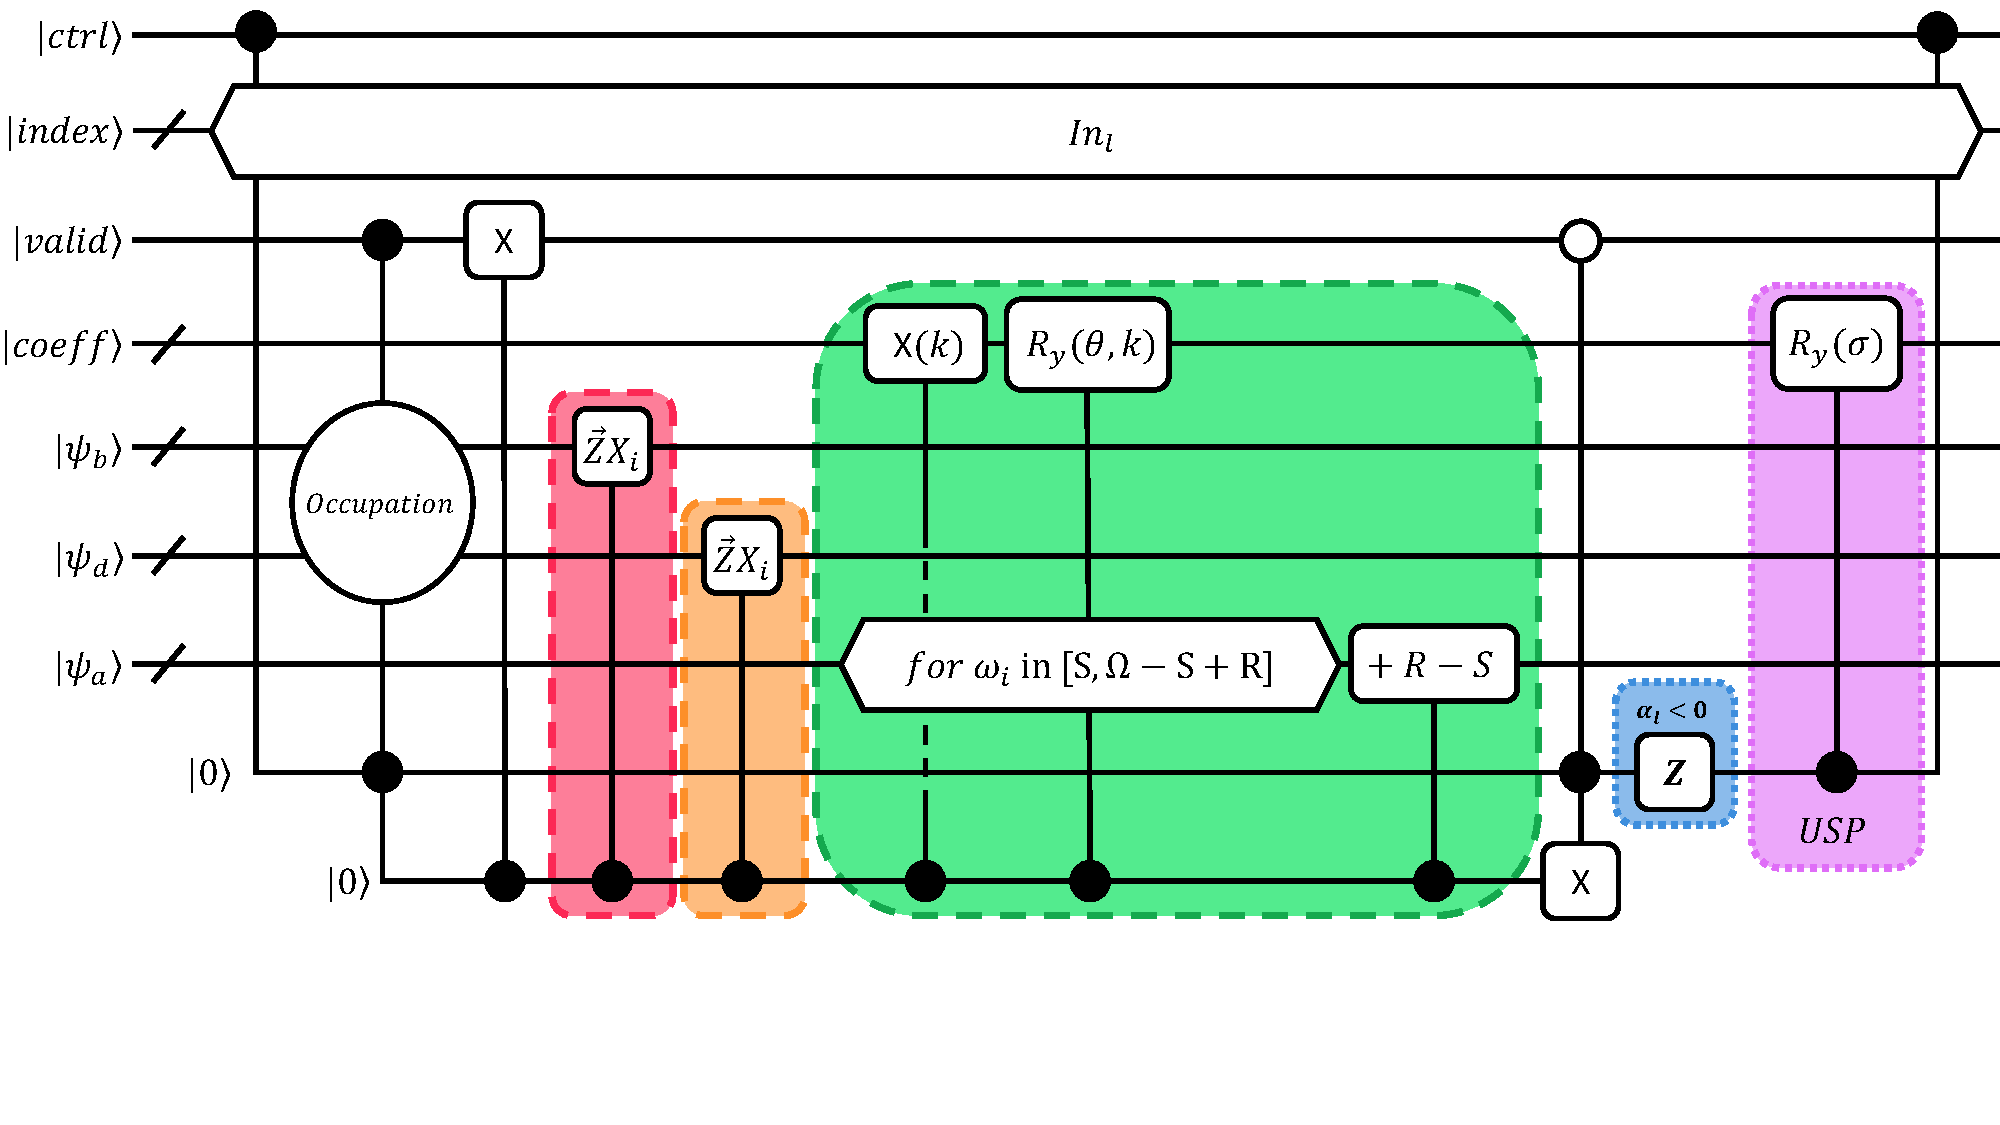
\includegraphics[width=16cm]{figures/select.pdf}
    \caption{
        \textbf{LOBE \textit{Select} Oracle (Decomposed)}
        This figure gives a schematic for constructing the components of the \textit{Select} oracle wherein the term $\Tilde{T_l}$ is applied onto the system register when the index register is in the computational basis state $\ket{l}$.
        The shaded red box with the dashed border show the update on the fermionic system when a fermionic ladder operator is applied.
        A similar series of operations is repeated for each fermionic ladder operator acting on the $i^{th}$ fermionic mode within the $l^{th}$ term.
        Similarly, the shaded orange box with the dashed border represent the application of antifermionic ladder operators and is also repeated for each antifermionic ladder operator within the $l^{th}$ term.
        The shaded green box with the dashed border depicts the application of all ladder operators acting on the $i^{th}$ bosonic mode.
        A similar series of operations is repeated for each bosonic mode with ladder operators acting upon it within the $l^{th}$ term.
        The hexagons in this box along with the $R_y(\theta, k)$ rotations depict controlled, multiplexed rotations and are implemented as described in Appendix \ref{sec:multiplexed-rotations}.
        The shaded blue box with the dotted border is applied when the coefficient of the $l^{th}$ term is negative.
        The ancilla qubit that it is applied on is in the $\ket{1}$ state whenever the $l^{th}$ term is applied and the Pauli-Z gate gives a phase of $-1$ on the amplitude of the associated quantum state.
        Finally, the shaded purple box with the dotted border is used to apply the magnitude of the coefficient associated with the $l^{th}$ term.
        These operations are \textit{only} included when the \textit{USP} protocol is used for \textit{Prepare}.
    }
    \label{fig:select}
\end{figure}

The \textit{Select} oracle is shown in Figure \ref{fig:lobe} as the oracle within the blue shaded region.
As is done in standard LCU circuits, the \textit{Select} oracle is designed such that it applies the term $T_l$ onto the system when the index register is in the computational basis state $\ket{l}$.
In Figure \ref{fig:select}, we give a circuit diagram for \textit{Select} focusing on the application of a single term, $T_l$.
The \textit{Select} oracle can be constructed by applying the circuit for each term ($T_l$) when the ancilla qubit of the multiplexing operator over the index register is in the computational basis state $\ket{l}$.

Throughout this work, the hexagonal boxes in circuit diagrams will represent multiplexors or coherent for-loops over the computational basis states of the registers on which they are applied..
An explicitly compiled circuit diagram for a controlled multiplexor is given in Figure 7 of \cite{babbush2018encoding} using approximately $L$ left and right elbows and $\lceil \log_2{L} \rceil$ ancillae qubits.
However, for the particular case of multiplexing when the applied unitary at each index is a rotation around the same axis, we use the compilation strategy of \cite{mottonen2004transformation} which is elaborated upon in Appendix \ref{sec:multiplexed-rotations}.

Working from left to right, the first operation shown in Figure \ref{fig:select} is the left-elbow of the controlled multiplexor over the index register.
This puts the ancilla qubit in the $\ket{1}$ state when the index register is in the computational basis state $\ket{l}$.
The gate cost of this controlled multiplexor is approximately:
\begin{equation}
    C_{\text{multiplex: index}} = (0, L, L)
\end{equation}
and requires the following clean ancillae:
\begin{equation}
    Q_{\alpha}^{\text{multiplex: index}} = \lceil \log_2{L} \rceil
\end{equation}

Next, a left-elbow - controlled on the validation qubit being in the $\ket{1}$ state, the index register being in the $\ket{l}$ state (determined by the previous ancilla qubit), and the system being in a state that will not be annihilated - is applied to produce a new ancilla qubit.
This ancilla qubit represents a quantum boolean that determines if the term $T_l$ should be applied onto the system in this branch of the wavefunction without zeroing-out the state.
To perform a check on if the state will be annihilated, controls are added based on the occupation of the fermionic and antifermionic modes corresponding to the operators that are present within the current term.
For each fermionic (antifermionic) creation operator acting on mode $i$, a $0$-control is added on $i^{th}$ fermionic (antifermionic) mode within $\ket{\psi_b}$ ($\ket{\psi_d}$).
Likewise, for each fermionic (antifermionic) annihilation operator acting on mode $i$, a $1$-control is added on $i^{th}$ fermionic (antifermionic) mode within $\ket{\psi_b}$ ($\ket{\psi_d}$).
If both ladder operators are present, then only the $1$-control on the $i^{th}$ mode remains since the state gets zeroed-out only if the mode is unoccupied (assuming that the term is normal ordered).
If any of these conditions are not satisfied, then the state should be zeroed-out and the ancilla qubit will remain in the $\ket{0}$ state for that branch of the wavefunction.
The quantum states that should be zeroed-out due to the bosonic operators will be handled when applying the coefficients of the bosonic operators to the system (green shaded box).

In total, this operation will have $2 + B_l + D_l$ controls for the term $T_l$, incurring the following cost (Eq. \ref{eq:N-ctrl-elbow}):
\begin{equation}
    C_{\text{term-boolean}} = (0, 1 + B_l + D_l, B_l + D_l)
\end{equation}
The maximum number of clean ancillae that will be required for this is:
\begin{equation}
    Q_\alpha^{\text{term-boolean}} = 1 + B
\end{equation}
with all but the output boolean qubit being immediately cleaned after the variable is computed.

After these checks are performed, the bottom ancilla qubit will be in the $\ket{1}$ state if and only if the three conditions are met.
This indicates that the term $T_l$ should be applied onto the system and that the fermionic ladder operators will not zero-out the state.
If the ancilla is in the $\ket{1}$ state, the validation qubit is first flipped from $\ket{1}$ to $\ket{0}$ to put the appropriate branch of the wavefunction into the encoded subspace.
This operation is a Clifford and therefore the gate cost is negligible and no ancillae are required.

The term $T_l$ is then applied to the system registers as portrayed in the shaded boxes with the dashed borders in Figure \ref{fig:select}.
All operations for applying the term $T_l$ (shaded boxes with dashed borders) will be controlled on this ancilla qubit determining if the term should be applied.
We will omit this clarification regarding the control on the following operations from the text for brevity.

The first shaded box (red) in Figure \ref{fig:select} shows the update on the fermionic system corresponding to a single creation or annihilation operator acting on the $i^{th}$ mode.
Since both the creation and annihilation operators flip the occupation and apply a phase - dependent on the parity of the occupation of the preceeding modes - they can both be applied using the same circuit.
To apply the appropriate phase, Pauli $Z$ gates are applied on all the fermionic modes for $j < i$.
To flip the occupation of the mode that the ladder operator acts on, a Pauli $X$ gate is applied to the $i^{th}$ fermionic qubit.
This series of gates is repeated for all fermionic creation or annihilation operators.
Many of these gates could be compiled out of the circuit, however, they are all Clifford operations and therefore will not significantly contribute to the cost of the block-encoding.
The second shaded box (orange) in Figure \ref{fig:select} portays the application of an antifermionic ladder operator and is constructed in an analogous way, but acts on the corresponding antifermionic modes.
All of these operations are Cliffords and likewise we exclude their gate-cost from our analysis.
They also do not require the use of any additional ancillae.

Next, the third shaded box (green) in Figure \ref{fig:select} depicts the action of bosonic ladder operators acting on the $i^{th}$ bosonic mode of the system.
This box is repeated for each bosonic mode that is being acted upon within the current term.
We will define our construction assuming that each term has be normal-ordered, however, we note that the construction presented here can generalize to terms that are not normal ordered with slight modifications.

Let any series of (normal-ordered) bosonic operators acting on the $i^{th}$ mode be described by:
\begin{equation}
    (a_i^\dagger)^R (a_i)^S
\end{equation}
where $R$ and $S$ are nonzero integers in the range $[0, \Omega]$.
The subscripts $*_{l, i}$ will be omitted from $S$ and $R$ in this section for brevity, but are implied.
The action of the rescaled operator on the state of the $i^{th}$ bosonic mode with initial occupation $\omega_i$ is given by:
\begin{equation}
    \label{eq:bosonic-operator-action}
    (a_i^\dagger)^R (a_i)^S \ket{\omega_i} = \prod_{r=0}^{R-1} \big( \sqrt{\frac{\omega_i - S + r + 1}{\Omega + 1}} \big) \prod_{s=0}^{S-1} \big( \sqrt{\frac{\omega_i - s}{\Omega + 1}} \big) \ket{\omega_i + R - S}
\end{equation}

This operation can implemented in the block-encoding via a quantum circuit as follows with $m$ denoting the number of bosonic modes that have already been applied in this term:
\begin{algorithmic}[1]
    \State Let $\ket{\text{anc}}_\text{fire}$ indicate if $T_l$ should be applied onto the quantum state
    
    \For{$\ket{m} \in [0, M-1]$}

        \If{$\ket{\text{anc}}_\text{fire} == \ket{1}$}
            \State $\ket{0}_m \gets X \ket{0}_m = \ket{1}_m$
            \For{Multiplex: $\omega_i \in S \leq \omega_i \leq \min(\Omega, \Omega - S + R)$}
                \State $\ket{1}_m \gets R_y(\theta) \ket{1}_m$
            \EndFor

            \State $\ket{\omega_i} \gets \ket{\omega_i + R - S}$
        \EndIf
    \EndFor
\end{algorithmic}
where $\ket{\text{anc}}_\text{fire}$ represents the bottom ancilla qubit in Figure \ref{fig:select}.

The application of a Pauli-X gate on the $m^{th}$ qubit in the coefficient register is used to rotate that qubit completely outside of the encoded subspace.

For the multiplexor over the occupation states, any state beginning with an occupation less than $S$ will be zeroed-out and therefore can be left outside of the encoded subspace by setting the rotation angle to zero.
Likewise, any state that should \textit{end} with an occupation greater than $\Omega$ will also be zeroed-out and therefore can also be left unmodified by setting the rotation angle to zero.
For occupation states inside the allowable range, the purpose of the rotations is to rotate the $m^{th}$ qubit in the coefficient register back into the encoded subspace with an amplitude in the $\ket{0}$ state equal to the amplitude in Eq. \ref{eq:bosonic-operator-action}:
\begin{equation}
    \label{eq:smarter-rot-angle}
    \theta(\omega_i, S, R) = 2 \sin^{-1}{\Big(\prod_{r=0}^{R-1} \big( \sqrt{\frac{\omega_i - S + r + 1}{\Omega + 1}} \big) \prod_{s=0}^{S-1} \big( \sqrt{\frac{\omega_i - s}{\Omega + 1}} \big)\Big)}
\end{equation}

This desired action is performed by the application of an Ry rotation on the $m^{th}$ qubit in the coefficient register by the angle $\theta$ given in Eq. \ref{eq:smarter-rot-angle}.
The implementation for these controlled-multiplexed rotations is discussed in more detail in Appendix \ref{sec:multiplexed-rotations}.
The gate cost for one of these controlled-multiplexed rotations is given by:
\begin{equation}
    \begin{split}
        C_{\text{bosonic-multiplex-rotations}} &= (2 + 2^{\lceil \log_2(\Omega) \rceil}, 2^{\lceil \log_2(\Omega) \rceil}, 2^{\lceil \log_2(\Omega) \rceil}) \\
        &\approx (2 + \Omega, \Omega, \Omega)
    \end{split}
\end{equation}
and requires one additional clean ancilla qubit that is immediately cleaned.
% \begin{equation}
%     Q_\alpha^{\text{bosonic-multiplex-rotations}} = 1
% \end{equation}

The update of the occupation states is implemented via a controlled-quantum addition operation that is discussed in Appendix \ref{sec:addition}.
With the classical value that is added being $+ R - S$, this contributes a gate cost of:
\begin{equation}
    C_{+ R - S} = (0, \lceil \log_2{\Omega + 1} \rceil - p - 1, \lceil \log_2{\Omega + 1} \rceil - p - 1)
\end{equation}
with $p$ determined by the binary representation of $+ R - S$ as described in Appendix \ref{sec:addition}.
This operation also requires $2(\lceil \log_2{\Omega + 1} \rceil - p) - 1$ clean ancillae which are immediately cleaned after the operation.
% \begin{equation}
%     Q_\alpha^{+ R - S} = 2(\lceil \log_2{\Omega + 1} \rceil - p) - 1
% \end{equation}

Since these operations are repeated $M_l$ times for the term $T_l$, the total gate cost is given by:
\begin{equation}
    C_\text{bosonic-updates} \approx \sum_m (2 + \Omega, \Omega + \lceil \log_2{\Omega + 1} \rceil - p_m - 1, \Omega + \lceil \log_2{\Omega + 1} \rceil - p_m - 1)
\end{equation}
and a number of clean ancillae upper-bounded by:
\begin{equation}
    \label{eq:ancillae-bosonic-updates}
    Q_\text{bosonic-updates} \leq 2 \lceil \log_2{\Omega + 1} \rceil - 1
\end{equation}
% This operation can implemented in the block-encoding via a quantum circuit as follows with all operations controlled on the ancilla qubit indicating if the current term should be applied, with $k$ denoting the number of bosonic modes that have already been accoutned for in this term:
% \begin{enumerate}
%     \item Apply a Pauli-X gate on the $k^{th}$ qubit in the coefficient register to rotate it completely outside of the encoded subspace.
%     \item Multiplex over the occupation of the $i^{th}$ bosonic mode for occupation states in the range: $S \leq \omega_i \leq \min(\Omega, \Omega - S + R)$. Any state beginning with an occupation less than $S$ will be "zeroed-out" and therefore can be left outside of the encoded subspace without any additional operations. Likewise, any state that should \textit{end} with an occupation greater than $\Omega$ will also be "zeroed-out" and therefore can also be left unmodified.
%     \item For each value of $\omega_i$ in the multiplexor, apply a rotation on the $k^{th}$ qubit in the coefficient register of angle $\theta$ given by Eq. \ref{eq:smarter-rot-angle}. The purpose here will be to rotate the qubit back into the encoded subspace with an amplitude in the $\ket{0}$ state equal to the amplitude in Eq. \ref{eq:bosonic-operator-action}. 

%     \begin{equation}
%         \label{eq:smarter-rot-angle}
%         \theta(\omega_i, S, R) = 2 \sin^{-1}{\Big(\prod_{r=0}^{R-1} \big( \sqrt{\frac{\omega_i - S + r + 1}{\Omega + 1}} \big) \prod_{s=0}^{S-1} \big( \sqrt{\frac{\omega_i - s}{\Omega + 1}} \big)\Big)}
%     \end{equation}

%     \item Update the occupation by a value of $+ R - S$. If $R = S$, no update is needed.
% \end{enumerate}
% Overall, this requires one multiplexor and one qubit in the coefficient register for each bosonic mode that is being acted upon within the term.
% The multiplexors will also have a reduced number of occupation modes to multiplex over, thereby reducing the number of Toffolis required for each multiplexor.

Once the state of the system is updated and the bosonic coefficients have been applied, the bottom ancilla qubit can be uncomputed (reset to $\ket{0}$).
This can be achieved by applying a Toffoli onto this qubit with a zero-control on the validation qubit and a one-control on the ancilla qubit used for multiplexing over the index register.
This Toffoli gate can be decomposed into one pair of elbows using one ancilla qubit that is immeidately cleaned:
\begin{equation}
    C_{\text{clean: term-boolean}} = (0, 1, 1)
\end{equation}
\ws{It's not quite clear to me if we can use a right-elbow here instead of a Toffoli since we are changing the states of fermionic/antifermionic modes after the left-elbow. Obviously it's only one Toff so it's not a big deal, but I wanna try to do some derivations for this.}

Next, if the sign of the coefficient of the current term is $-1$, we apply a $- \mathds{1}$ - controlled on the index register being in the state $\ket{l}$ - to the state, regardless of which \textit{Prepare} oracle is used.
This operation is shown in the fourth shaded box (blue) with the dotted border to indicate that this operation may or may not be present depending on the sign of the term.
This can be achieved in many ways, but here we simply use a Pauli-Z gate acting on the ancilla qubit storing the state of the multiplexor acting on the index register.
This is only Clifford gates and does not require any ancillae.

Finally, if the \textit{uniform state perparation} protocol is used for the \textit{Prepare} oracle, then the normalized coefficient of the term must be applied.
This is achieved via a controlled Pauli-Y rotation that is applied onto the final qubit in the coefficient register (this is the qubit that does not get touched by the bosonic updates).
This is shown in the fifth shaded box (purple) with the dotted border to indicate that this operation may or may not be present depending on which \textit{Prepare} oracle is used.
This rotation is used to account for the rescaled coefficient of the term ($\Tilde{\alpha_l}$) and is achieved by applying a rotation with an angle given by:
\begin{equation}
    \sigma(\Tilde{\alpha_l}) \equiv 2 \cos^{-1}{|\Tilde{\alpha_l}|}
\end{equation}
If the \textit{arbitrary state preparation} protocol is used, then this rotation is not needed as the coefficient of the term is already accounted for and one fewer qubit is needed in the coefficient register.
A controlled rotation may be perfomed with two rotations and two CNOT gates, thereby incurring the following cost:
\begin{equation}
    C_{\Tilde{\alpha_l}}^\text{USP} = (2, 0, 0)
\end{equation}
where the $*^\text{USP}$ superscript indicates that this cost is only included when \text{USP} is used for \textit{Prepare}.

In total, the approximate number of clean ancillae required is given by:
\begin{equation}
    \begin{split}
        Q_\alpha &= 2 + \lceil \log_2{L} \rceil + \max{(2 \lceil \log_2{\Omega + 1} \rceil - 1, B, 1)} \\ 
    \end{split}
\end{equation}
where $2$ ancillae are used to store the quantum booleans in Figure \ref{fig:select}, $B$ are temporarily used for computing the ``term-boolean'', $2 \lceil \log_2{\Omega + 1} \rceil - 1$ are temporarily used for the update of the bosonic occupancy, $1$ is temporarily used in many of the operations such as the controlled-multiplexed rotations and the Toffoli to reset the quantum boolean.
Under the assumption that $2 \lceil \log_2{\Omega + 1} \rceil - 1 > B > 1$, the maximum number of ancillae required is given by:
\begin{equation}
    Q_\alpha \approx 1 + \lceil \log_2{L} \rceil + 2 \lceil \log_2{\Omega + 1} \rceil
\end{equation}

The total qubit requirement under these compilation choices - disregarding the control qubit and the optional qubit required when $USP$ is used - is given by:
\begin{equation}
    \begin{split}
        Q &= Q_{\textit{index}} + 1 + Q_{\textit{coeff}} + Q_{\psi_b} + Q_{\psi_d} + Q_{\psi_a} + Q_\alpha \\
        &\approx \lceil \log_2{L} \rceil + 1 + M + 2I + I\lceil \log_2{(\Omega + 1)} \rceil + 1 + \lceil \log_2{L} \rceil + 2 \lceil \log_2{\Omega + 1} \rceil \\
        &\approx 2(\lceil \log_2{L} \rceil) + (I + 2)\lceil \log_2{(\Omega + 1)} \rceil + 2I + M + 2
    \end{split}
\end{equation}
which is linear in the number of modes and logarithmic in the number of terms and the bosonic occupation cutoff.

The cost of the \textit{Select} oracle for LOBE, $C_{\textit{Select}}$, can be computed as a sum of the individual costs outlined above:
\begin{equation}
    \begin{split}
        C_{\textit{Select}} &= C_{\text{multiplex: index}} + \sum_l (C_{\text{term-boolean}} + C_\text{bosonic-updates} + C_{\text{clean: term-boolean}}) \\
        &\begin{split}
            &\approx (0, L, L) \\
            &+ \sum_l (0, 1 + B_l + D_l, B_l + D_l) \\
            &+ \sum_l \sum_m (2 + \Omega, \Omega + \lceil \log_2{\Omega + 1} \rceil - p_m - 1, \Omega + \lceil \log_2{\Omega + 1} \rceil - p_m - 1) \\
            &+ \sum_l (0, 1, 1) \\ 
        \end{split} \\
    \end{split}
\end{equation}
Though the exact gate counts are not clear from this expression, we can see that the asymptotic gate counts are given by:
\begin{equation}
\begin{split}
    N_\text{rot} &= O(LM \Omega) \\
    N_\text{elbow} &= O\big(L + LI + LM(\Omega + \log{\Omega}) \big)
\end{split}
\end{equation}
where $M$ is upper-bounded by $I$.

For the overall gate counts, we will focus on the variant using Grover-Rudolph to implement \textit{ASP}, however it is straightforward to compute the associate gate counts for $\text{USP}$.
Beginning from Figure \ref{fig:lobe}, we can compute the overall gate cost of the block-encoding as $2*C_{GR} + C_{\textit{Select}}$.

% Since the $\textit{Prepare}$ oracle for $USP$ is simply a string of Hadamard gates, this oracle contributes no non-Cliffords and $C_{\textit{USP}} = (0, 0, 0, 0)$.
% In Appendix \ref{sec:grover-rudolph}, we discuss the gate cost for the implementation of Grover-Rudolph used in this work. \ws{Fill this out once gate cost is better understood.}

% For the cost of the $\textit{Select}$ oracle, we will focus on the form when using $USP$ for $\textit{Prepare}$.
% When Grover-Rudolph is used instead, the only change to the $\textit{Select}$ oracle is that the controlled rotation is not included and therefore the rotation count is reduced accordingly.  

% The cost of the controlled-multiplexor over the index register is given by $L - 1$ left (and right) elbows \cite{babbush2018encoding} where $L$ is the number of terms in the Hamiltonian or the number of computational basis states we are interested in.
% This accounts for the cost of generating the quantum boolean second from the bottom in Figure \ref{fig:select}.
% No rotations or additional Toffolis are required, therefore the cost is given by: 
% \begin{equation}
%     C_{\textit{index}} = (0, 0, L-1, L-1)
% \end{equation}

% The rest of the gate cost of the $\textit{Select}$ oracle can be computed as the sum of the cost of implementing the individual terms:
% \begin{equation}
%     C_{\textit{Select}} = C_{\textit{index}} + \sum_{l} C_{T_l}
% \end{equation}

% The first operation performed for each term is the computation of the bottom qubit in Figure \ref{fig:select}.
% This quantum boolean is computed via a left-elbow with $B_l + D_l + 2$ controls where $B_l$ and $D_l$ represent the number of fermionic and antifermionic modes being acted upon within the term $T_l$.
% As was mentioned in Subsubsection \ref{subsubsec:space}, this multi-controlled operation can be decomposed into $B_l + D_l + 1$ left elbows and $B_l + D_l$ right elbows.

% Flipping the validation qubit and performing the fermionic and antifermionic operators only require Cliffords and therefore do not contribute to the gate counts we are interested in.

% Next, we have the cost of implementing the bosonic operators.
% For each of the $M_l$ bosonic modes being acted upon within the term $T_l$, we must perform a controlled-multiplexor over the $\Omega - 2S_{l, m} + R_{l, m}$ non-trivial occupation states of the mode being acted upon.
% Where $l$ indexes the term in the Hamiltonian and $m$ indexes the bosonic mode being acted upon within the $l^{th}$ term.
% This will require $\Omega - 2S_{l, m} + R_{l, m} - 1$ left (and right) elbows and for each nontrivial occuptation state, a controlled rotation will be performed.
% Therefore, we can sum up the cost of implementing all of the $M_l$ bosonic operators as: 
% \begin{equation}
%     C_{M_l} = \Big(\Sigma_l, 0, \Sigma_l - M_l, \Sigma_l - M_l \Big)
% \end{equation}
% where $\Sigma_{l} \equiv \Omega - 2S_{l, m} + R_{l, m}$.

% \ws{Add cost of adding classical values to bosonic registers here. Will cost a decent number of Toffolis.}

% Uncomputing the bottom ancilla qubit requires one Toffoli. \ws{still not sure if this can be replaced by a right-elbow.}
% Lastly, when $USP$ is used for $\textit{Prepare}$, a controlled rotation is performed.
% Therefore, the overall cost of implementing a single term \ws{temporarily neglecting the cost of incrementing/decrementing} is given by:
% \begin{equation}
%     C_{T_l} = \Big(1 + \Sigma_l, 1, B_l + D_l + 1 + \Sigma_l - M_l, B_l + D_l + \Sigma_l - M_l \Big)
% \end{equation}

% Therefore, the overall cost of implementing the $\textit{Select}$ oracle is given by:
% \begin{equation}
%     \begin{split}
%     C_{\textit{Select}} &= C_{\textit{index}} + \sum_{l} C_{T_l} \\
%     &= \Big(L + \sum_l \Sigma_l, L, 2L - 1 + \sum_l \big( B_l + D_l + \Sigma_l - M_l \big), L-1 + \sum_l \big( B_l + D_l + \Sigma_l - M_l \big)\Big)
%     \end{split}
% \end{equation}

\section{Results}
\label{sec:results}

In this section, we demonstrate the use of LOBE to block-encode Hamiltonians derived from quantum field theories: Yukawa theory and $\phi^4$ theory \cite{Peskin:1995ev}.
We study both variants of the block-encoding described in Sections \ref{sec:block-encoding} and expanded upon in Section \ref{sec:lobe} and give numerical counts for the numbers of non-Clifford operations, the number of ancillae required beyond the system register, and the rescaling factor imposed on the resulting block-encoding.

The results that we present here are generated based on constructions of LOBE that are written in Cirq \cite{cirq} and the block-encodings are numerically verified for circuits of up to 14 qubits.
Additionally, the operators are constructed through the use of OpenParticle \cite{openparticle}, a software library for the construction and manipulation of fermionic, antifermionic, and bosonic ladder operators.
The software library \cite{grover-rudolph-github} is used to determine the rotation angles required for Grover-Rudolph.

\subsection{Yukawa Theory}
A quantum field theory that models the strong nuclear force between hadrons is Yukawa theory \cite{Peskin:1995ev}. In this theory, hadrons are described by a fermionic field $\psi$, coupled via a scalar boson $\phi$. The interaction term is $\mathcal{L}_{\text{Yukawa}} = g\bar\psi \psi \phi$, which leads to interaction vertices containing fermions and/or antifermions and bosons. The Lagrangian, and thus the Hamiltonian, is written as a sum of free, non-ineteracting fields and the interaction term.

Utilizing the lightfront frame \cite{Dirac1949}, leads to a straightforward approach to writing down the Hamiltonian bound-state eigenvalue equation in terms of ladder operators. This lightfront frame removes the ambiguous $\sqrt{\nabla^2 + m^2}$ term that appears in a canonical, instant-time frame Hamiltonian approach. 

The interaction terms in the Hamiltonian are $H_{\text{Yukawa int}} \in \{b^\dagger b a, b^\dagger b a^\dagger, d^\dagger d a, d^\dagger d a^\dagger, b^\dagger d^\dagger a, bda^\dagger, b^\dagger b a^\dagger a, d^\dagger d a^\dagger a \}$, while the free part of the Hamiltonian is $H_{\text{free}} \in \{b^\dagger b, d^\dagger d, a^\dagger a \}$. 
Much of the interesting physics arises from the interacting piece. The terms $b^\dagger b a$ and $b^\dagger b a^\dagger$ describe the annihilation of a fermion with a boson and creation of a fermion, and the creation of a fermion-boson pair from a fermion respectively. $d^\dagger d a$ and $d^\dagger d a^\dagger$ describe the same interactions but for antifermions and bosons. 
$b^\dagger d^\dagger a$ and $bda^\dagger$ correspond to fermion-antifermion pair creation and annihilation, and lastly, $b^\dagger b a^\dagger a$ and $d^\dagger d a^\dagger a$ are terms of $\mathcal{O}(g^2)$, unique to the lighfront frame.

This Hamiltonian can be written out as a discrete sum over these free and interaction ladder operators with coefficients coming from lightfront coordinates. The Hamiltonian can be written as:

\begin{equation}
    \label{eq:Yukawa-hamiltonian}
    H_{\text{Yukawa}} = H_0 + H_{\bar\psi \psi \phi}.
\end{equation}
The explicit form of the Hamiltonian will be written out in the appendix. 

\begin{figure}
    \centering
    \includegraphics[width=16cm]{figures/Yukawa_hamiltonian_gates_vs_terms.pdf}
    \caption{
        \textbf{Numerical Gate Counts for Increasing $L$ (Yukawa Hamiltonian).}
        The number of rotations (left), left-elbows (middle), and right-elbows (right) are plotted as a function of the number of terms in the Hamiltonian ($L$) for an increasing number of momentum modes ($I$).
        The gate counts for the variant of LOBE using \textit{USP} are shown as the blue squares.
        The gate counts for the variant of LOBE using \textit{ASP} are shown as the orange circles.
        The bosonic occupancy cutoff ($\Omega$) is set to $3$.
        The number of rotations excludes rotations by angles that result in Clifford operations.
    }
    \label{fig:Yukawa_hamiltonian_gates_vs_terms}
\end{figure}
\begin{figure}
    \centering
    \includegraphics[width=12cm]{figures/Yukawa_hamiltonian_qubits_and_rescaling_vs_terms.pdf}
    \caption{
        \textbf{Numerical Ancillae Counts and Rescaling Factors for Increasing $L$ (Yukawa Hamiltonian).}
        The number of required ancillae (left) and the resulting rescaling factor (right) for LOBE are plotted as a function of the number of terms in the Hamiltonian ($L$) for an increasing number of momentum modes ($I$).
        The counts for the variant of LOBE using \textit{USP} are shown as the blue squares.
        The counts for the variant of LOBE using \textit{ASP} are shown as the orange circles.
        The bosonic occupancy cutoff ($\Omega$) is set to $3$.
    }
    \label{fig:Yukawa_hamiltonian_qubits_and_rescaling_vs_terms}
\end{figure}

In Figure \ref{fig:Yukawa_hamiltonian_gates_vs_terms}, we plot the numerical gate counts estimates for the Yukawa Hamiltonian (Eq. \ref{eq:Yukawa-hamiltonian}) as the number of terms in the Hamiltonain ($L$) increases.
The number of terms ($L$) increases directly with an increasing number of momentum modes as $\mathcal{O}(I^3)$
For the three non-Clifford operations, the number of operations increases linearly with the number of terms in the Hamiltonian for this model.
Additionally, the two different compilation strategies (\textit{USP} (blue), \textit{ASP} (orange)) demonstrate the same numerical scaling and have nearly identical gate counts for all types of operations.
When the number of terms ($L$) is far from the next largest power of 2, \textit{ASP} requires more arbitrary rotations due to the compilation of Grover-Rudolph and multiplexed rotations that is used in this work.

In Figure \ref{fig:Yukawa_hamiltonian_qubits_and_rescaling_vs_terms}, we plot the numerical estimates for the number of required ancillae (left) and the imposed rescaling factor (right) as the number of terms in the Hamiltonain ($L$) increases.
The number of ancillae grows logarithmically with the number of terms for both implementations.
The number of ancillae used for the index register grows logarithmically with the number of terms which accounts for this scaling.
The main advantage of the \textit{ASP} variant is the effect on the rescaling factor of the block-encoding.
While the rescaling factor of both variants seemingly grows linearly with respect to the number of terms in the Hamiltonian, the rescaling factor for the \textit{ASP} variant is significantly smaller than the \textit{USP} variant.
When block-encodings are employed as a subroutine in larger algorithms, the quantum resources for the algorithm are often dependent on the rescaling factor (with a lower rescaling factor generally being preferred).
For example, in the context of using Quantum Phase Estimation to estimate the eigenvalues of a Hamiltonian, the number of gates required typically scales as $O(\frac{1}{\lambda})$ \cite{babbush2018encoding}. 
However, the exact cost associated with the rescaling factor is difficult to determine without choosing a specific algorithm to benchmark with.

\begin{figure}
    \centering
    \includegraphics[width=16cm]{figures/Yukawa_hamiltonian_gates_vs_omega.pdf}
    \caption{
        \textbf{Numerical Gate Counts for Increasing $\Omega$ (Yukawa Hamiltonian) .}
        The number of rotations (left), left-elbows (middle), and right-elbows (right) are plotted as a function of the bosonic occupation cutoff ($\Omega$).
        The gate counts for the variant of LOBE using \textit{USP} are shown as the blue squares.
        The gate counts for the variant of LOBE using \textit{ASP} are shown as the orange circles.
        The number of momentum modes ($I$) is set to $2$.
        The number of rotations excludes rotations by angles that result in Clifford operations.
    }
    \label{fig:Yukawa_hamiltonian_gates_vs_omega}
\end{figure}
\begin{figure}
    \centering
    \includegraphics[width=12cm]{figures/Yukawa_hamiltonian_qubits_and_rescaling_vs_omega.pdf}
    \caption{
        \textbf{Numerical Ancillae Counts and Rescaling Factors for Increasing $\Omega$ (Yukawa Hamiltonian).}
        The number of required ancillae (left) and the resulting rescaling factor (right) for LOBE are plotted as a function of the bosonic occupation cutoff ($\Omega$).
        The counts for the variant of LOBE using \textit{USP} are shown as the blue squares.
        The counts for the variant of LOBE using \textit{ASP} are shown as the orange circles.
        The number of momentum modes ($I$) is set to $2$.
    }
    \label{fig:Yukawa_hamiltonian_qubits_and_rescaling_vs_omega}
\end{figure}

In Figure \ref{fig:Yukawa_hamiltonian_gates_vs_omega}, we plot the numerical gate counts estimates for the Yukawa Hamiltonian (Eq. \ref{eq:Yukawa-hamiltonian}) as the cutoff on the maximum bosonic occupation ($\Omega$) increases.
For the three non-Clifford operations, the number of operations increases linearly with the bosonic occupancy cutoff for this model.
Similar to the case with increasing $I$, the two different compilation strategies (\textit{USP} (blue), \textit{ASP} orange) demonstrate the same numerical scaling and have nearly identical gate counts for all types of operations.

In Figure \ref{fig:Yukawa_hamiltonian_qubits_and_rescaling_vs_omega}, we plot the numerical estimates for the number of required ancillae (left) and the imposed rescaling factor (right) as the cutoff on the maximum bosonic occupation ($\Omega$) increases.
The number of ancillae grows logarithmically with the bosonic occupation cutoff for both implementations.
The number of ancillae needed to update the bosonic occupancy grows logarithmically with $\Omega$ (Eq. \ref{eq:ancillae-bosonic-updates}) which accounts for this scaling.
Again, the main advantage of the \textit{ASP} variant is that the imposed rescaling factor is significantly smaller than the \textit{USP} variant, especially for large values of $\Omega$ despite the asymptotic scaling being linear for both.


\subsection{$\phi^4$ Theory}
\gus{@kamil}
\section{Conclusions}
\label{sec:conclusions}


\section{Acknowledgements}

Wop, wop, wop, wop, wop, Dot, fuck 'em up

Wop, wop, wop, wop, wop, I'ma do my stuff
\cite{Lamar_2024}

\bibliography{refs/citations}

\appendix

\section{Glossary}
\label{sec:glossary}

In this Section, we explicitly define some of the technical phrases and symbols used throughout this work.

\begin{itemize}
    \item \textit{term} ($T$): An operator defined as a product of ladder operators.
    \item \textit{Active Mode}: A fermionic or bosonic mode upon which a ladder operator is being non-trivially applied. 
    \item \textit{block-encoding ancillae}: A register of qubits that give additional degrees of freedom to produce a block-encoding for the operator in a larger Hilbert space.
    \item \textit{``zeroed-out"}: When the coefficient of a state becomes zero due to the application of an operator.
    \item \textit{encoded subspace}: The chosen subspace of the block-encoding ancillae that denotes the subspace in which the non-unitary operator is encoded. Typically, this is the subspace where all block-encoding ancillae are in the $\ket{0}$ state.
    \item \textit{clean ancillae}: A register of qubits that are promised to begin in the $\ket{0}$ and are returned to the $\ket{0}$ state at the end of a particular operation. 
    \item \textit{all-zero state}: A state of a register where all qubits are in the $\ket{0}$ state.
    \item $L$: The number of terms in the Hamiltonian.
    \item $\alpha_l$: The coefficient of the $l^\text{th}$ term in a linear combination. Assumed to be real and positive unless otherwise stated.
    \item $\Omega$: The occupation cutoff for the bosonic modes. $\Omega$ gives the maximum number of bosons that can be present in a single mode. 
    \item $I$: The number of fermionic or bosonic modes. The subscripts $b$ and $a$ will be used to denote the number of fermionic and bosonic modes respectively.
    \item $b_i$: Fermionic annihilation (creation - $b_i^\dagger$) operator acting on mode $i$.
    \item $d_i$: Antifermionic annihilation (creation - $d_i^\dagger$) operator acting on mode $i$.
    \item $a_i$: Bosonic annihilation (creation - $a_i^\dagger$) operator acting on mode $i$.
    \item $n_{i_b}$: The number of fermions ($b$) occupying the $i^{th}$ mode. $n_{i_d}$ and $n_{i_a}$ give the occupancy for antifermions and bosons respectively.
    \item $\omega_{i}$: The number of bosons occupying the $i^{th}$ bosonic mode.
    \item $N_A$: The dimension of a matrix $A$.
    \item $\beta_\psi$: The amplitude of a state that is outside of the encoded subspace after a block-encoding unitary is applied to $\ket{\psi}$.
    \item $\lambda$: The rescaling factor imposed on the operator for a given block-encoding.
    \item $w$: The index of the $w^\text{th}$ least-significant bit in a binary encoding.
    \item $B$: The number of active modes within a term. The  with ladder operators acting on them within the term $T_l$.
    \item $C$: The number of active modes within a term \textit{excluding} modes upon which a number operator is being applied.
    \item $S_{l, i}$: The exponent of bosonic annihilation operators acting on the $i^{th}$ bosonic mode within the $l^{th}$ term.
    \item $R_{l, i}$: The exponent of bosonic creation operators acting on the $i^{th}$ bosonic mode within the $l^{th}$ term.
    \item $P$: The sum of the exponents of bosonic ladder operators acting on all modes within a single term.
\end{itemize}
\section{Proof of $\lambda_{ASP} \leq \lambda_{USP}$}
\label{sec:proof-of-rescaling-factors}

\begin{theorem}
    $\lambda_{ASP} \leq \lambda_{USP}$
\end{theorem}

\textbf{Proof:} 

Define the following:
\begin{equation}
    \lambda_{USP} \equiv L\max_l|\tilde{\alpha}_l|
\end{equation}
and
\begin{equation}
    \lambda_{ASP} = \sum_l |\tilde{\alpha}_l|
\end{equation}

\textit{Case 1: All Coefficients are Equal}

Assume $\tilde{\alpha}_i = \tilde{\alpha}_j \forall i,j$.
Let $\tilde{\alpha}_i = \tilde{\alpha}$.
Then, $\lambda_{USP} \equiv L\max_l|\tilde{\alpha}_l| = L|\tilde{\alpha}|$ and $\sum_{l = 0}^{L - 1}|\tilde{\alpha}_l| = L|\tilde{\alpha}|$.
Thus, in this case, $\lambda_{USP} = \lambda_{ASP}$.

\textit{Case 2: Coefficients are Not All Equal}

Assume that there exist at least two coefficients, $\tilde{\alpha}_i$ and $\tilde{\alpha}_j$ such that $\tilde{\alpha}_i \neq \tilde{\alpha}_j$.
This implies that at least one coefficient, $\alpha_l$, has the largest magnitude.
Then, $\lambda_{ASP} = max_l|\tilde{\alpha}_l| + \sum_{k \neq l}|\tilde{\alpha}_k|$.
Now, if $\lambda_{ASP} < \lambda_{USP}$, then $\lambda_{ASP} - \lambda_{USP} < 0$:
\begin{align}
    \lambda_{ASP} - \lambda_{USP} &= max_l|\tilde{\alpha}_l| + \sum_{k \neq l}|\tilde{\alpha}_k| - Lmax_l|\tilde{\alpha}_l|\\ \nonumber
                                &= -(L - 1)max_l|\tilde{\alpha}_l|+ \sum_{k \neq l}|\tilde{\alpha}_k| \\ \nonumber
                                &< -(L - 1)max_l|\tilde{\alpha}_l| + \sum_{k \neq l}max_l|\tilde{\alpha}_l| \\ \nonumber
                                &= -(L - 1)max_l|\tilde{\alpha}_l| + (L - 1) max_l|\tilde{\alpha}_l|\\ \nonumber
                                &= 0 \\ \nonumber
\end{align}

Therefore, $\lambda_{ASP} \leq \lambda_{USP}$.$\blacksquare$

\section{Quantum Addition}
\label{sec:addition}

Updating the occupancy of a bosonic mode when applying bosonic ladder operators requires adding a classical number ($+ R - S$) to the register storing the occupation of the bosonic mode.
Controlled (modular) addition of a two quantum registers (storing the numbers in binary) can be performed using $2N - 3$ left (and right) elbows and $M - 1$ ancillae using the construction for addition introduced in \cite{gidney2018halving} (Figure 4):
\begin{equation}
    (\alpha \ket{0} + \beta \ket{1})\ket{m}\ket{n} \rightarrow \alpha \ket{0}\ket{m}\ket{n} + \beta \ket{1}\ket{m}\ket{n \oplus m}
\end{equation}
where $m$ is the value being added to $n$ and $M$ and $N$ are the lengths of the registers respectively.

When performing a bosonic occupancy update, the value of $m$ is a known, \textit{classical} value ($+ R - S$).
Naively, this could be performed by loading the value of $m$ into a clean register and then performing controlled addition of the two registers as described above.
However, since the value of $m$ is classial and known, there are a few other options.

\begin{figure}
    \centering
    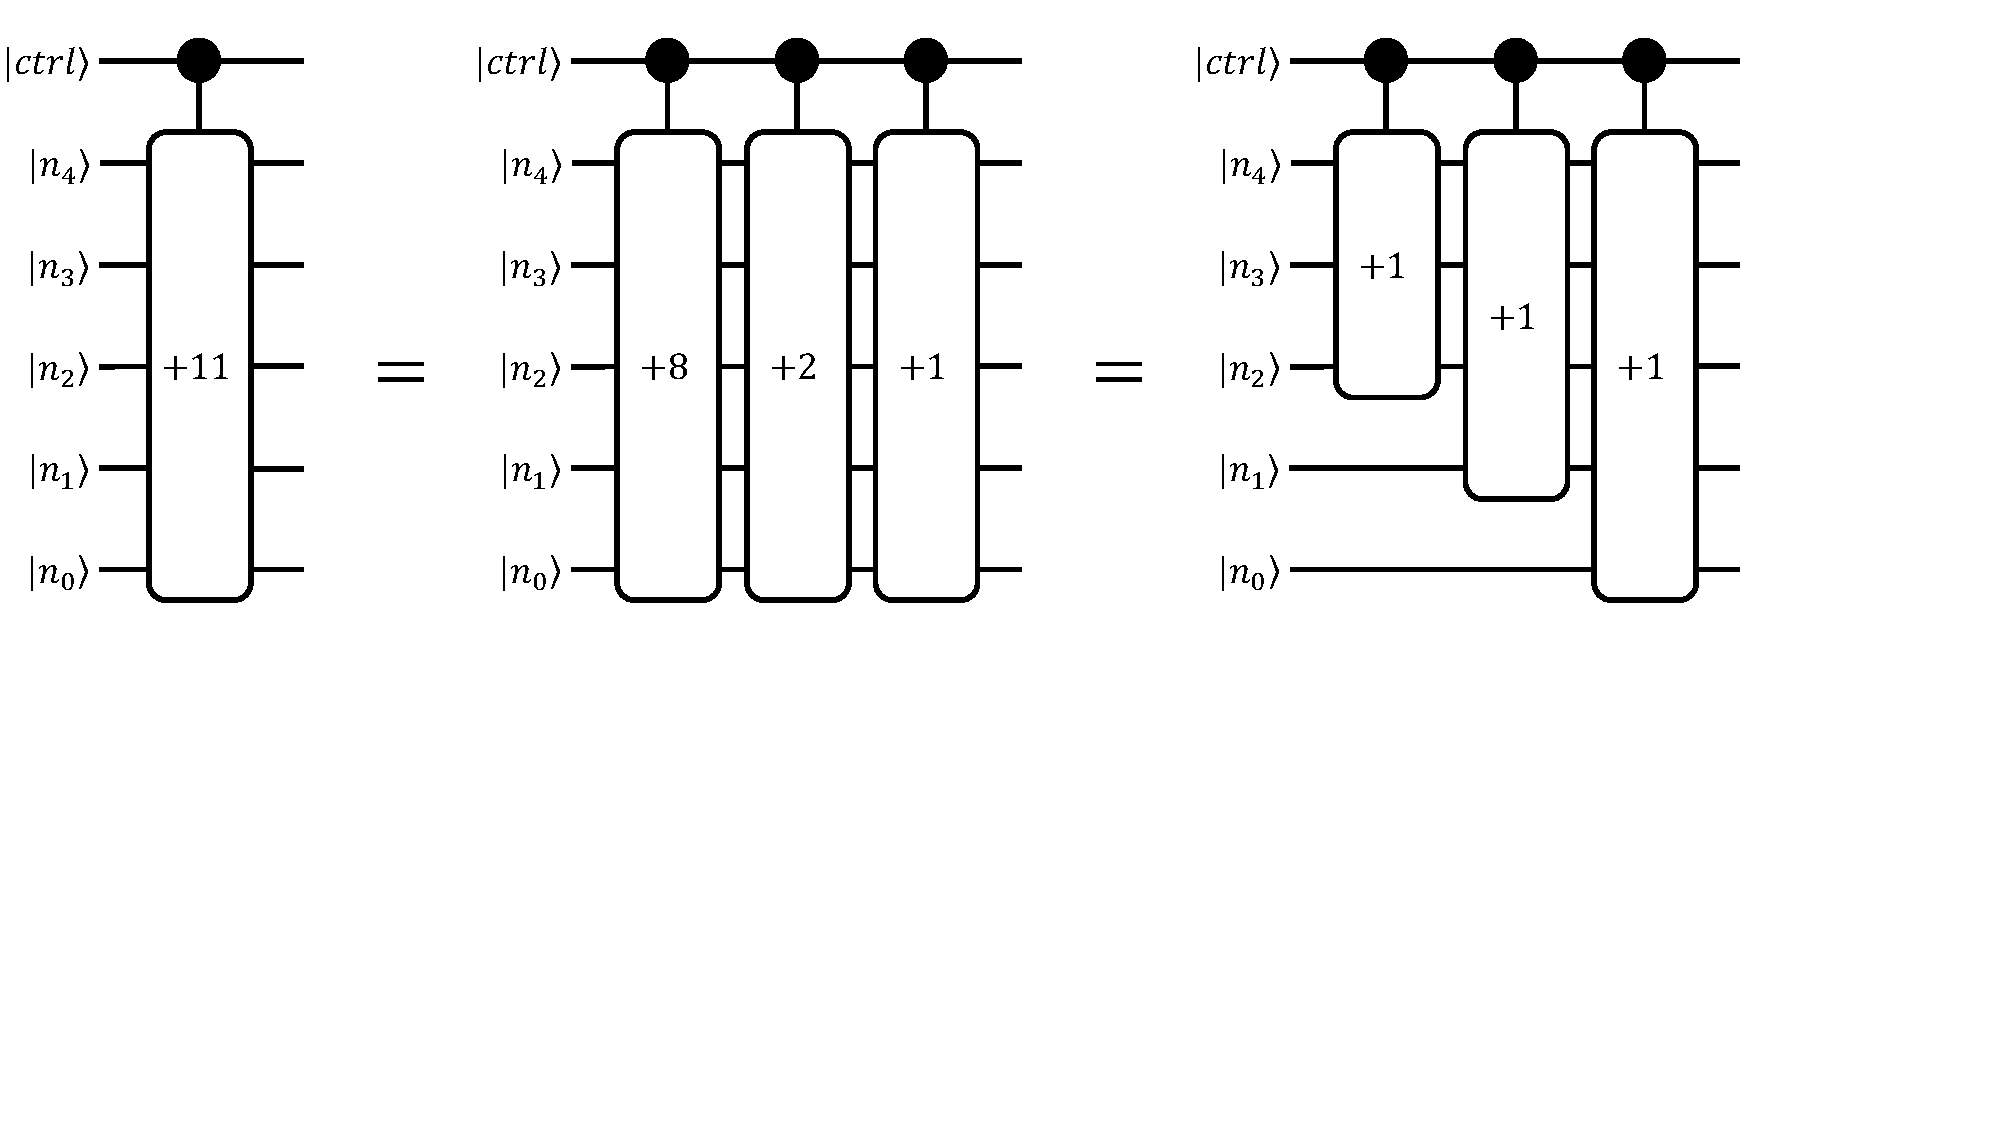
\includegraphics[width=16cm]{figures/addition-via-incrementers.pdf}
    \caption{
        \textbf{Addition via Controlled Incrementers.} 
    }
    \label{fig:addition-via-incrementers}
\end{figure}

\begin{figure}
    \centering
    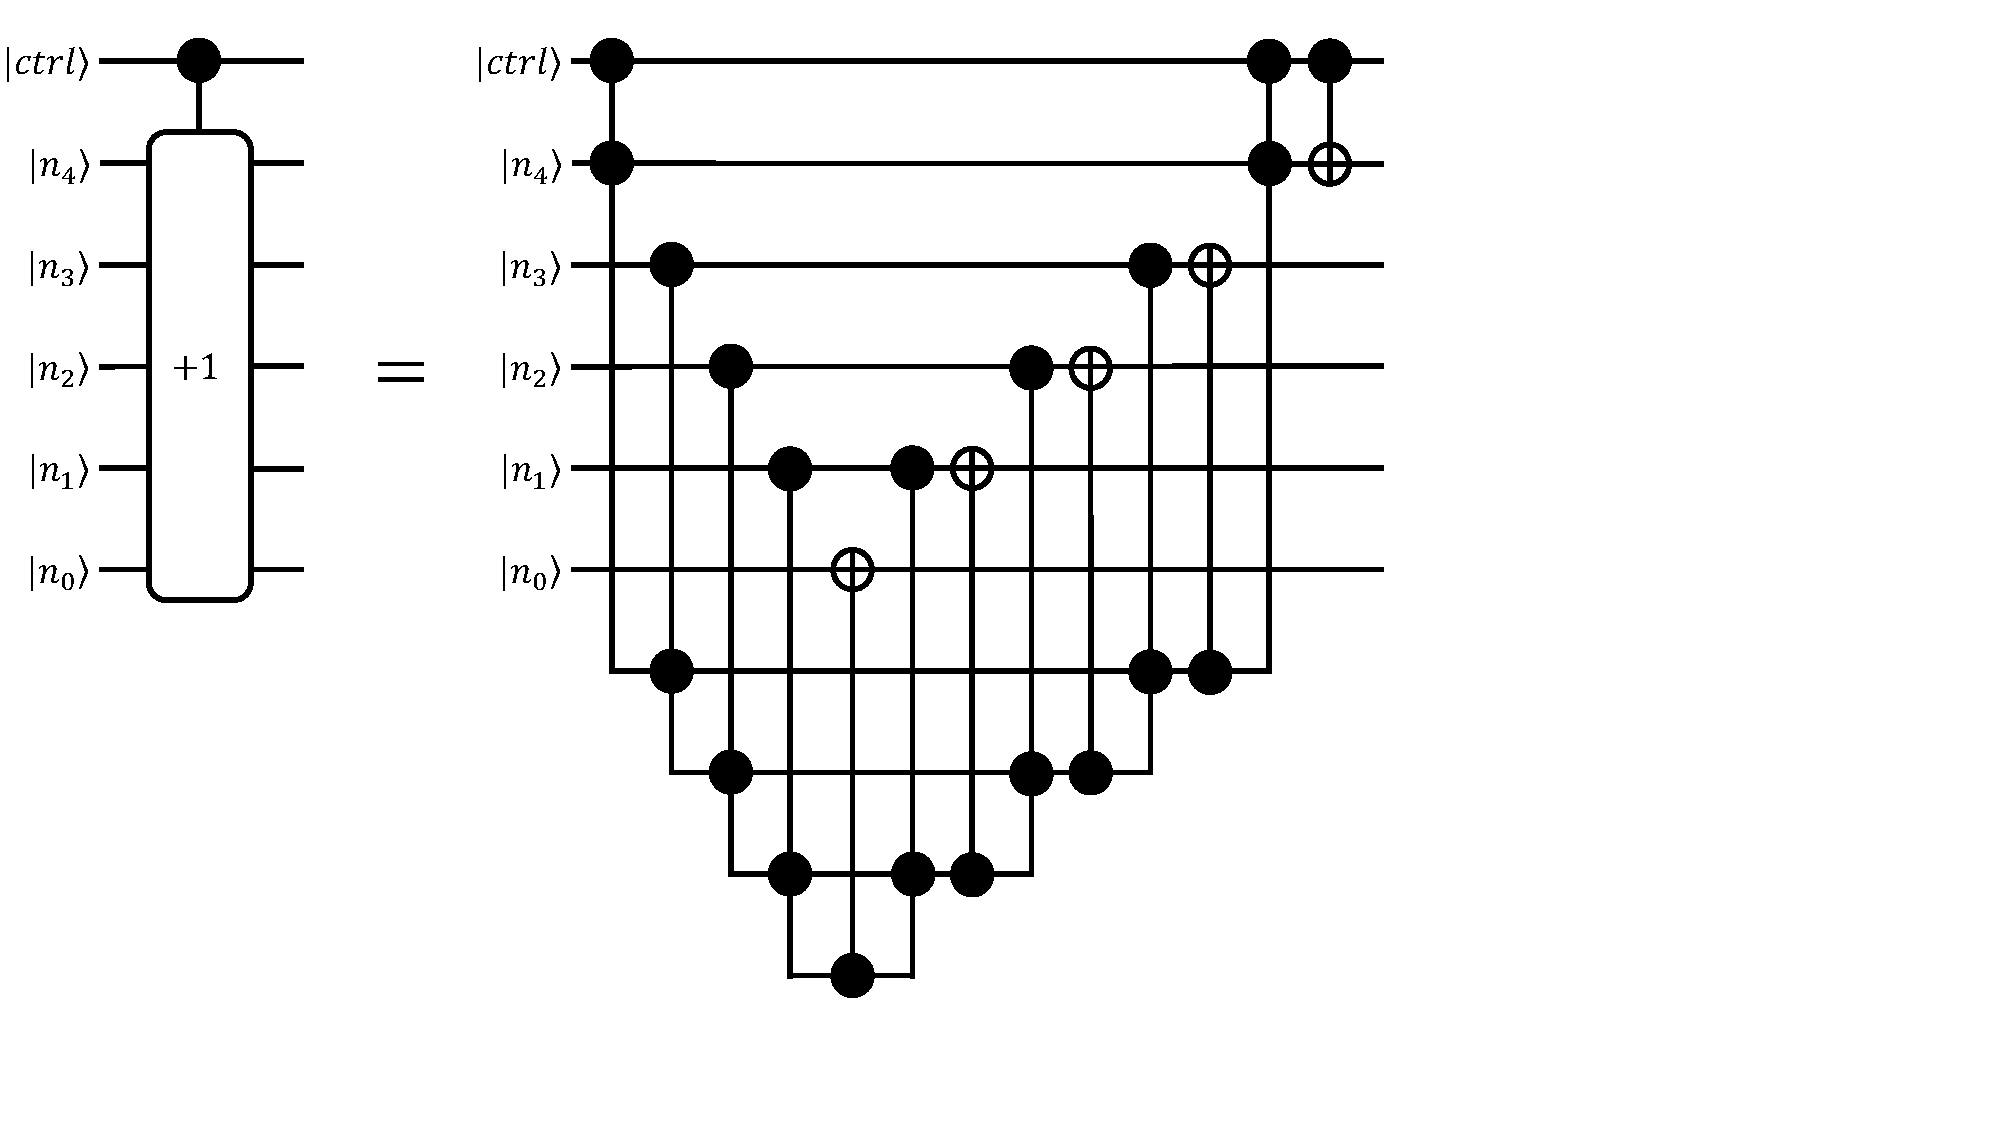
\includegraphics[width=8cm]{figures/incrementer.pdf}
    \caption{
        \textbf{Controlled Incrementer.} 
    }
    \label{fig:incrementer}
\end{figure}


One option is to use controlled incrementer ($+1$) circuits acting on different subsets of the register in order to construct the overall addition.
An incrementer circuit can be used to perform addition by a power of $2$ by shifting the qubits that the incrementer acts on.
For example, a circuit for adding the value $8$ to a register in binary can be performing using an incrementer circuit that treats the $4^{th}$ least significant qubit as the least significant qubit in the incrementer circuit and disregards the $3$ lesser qubits.
A circuit adding any classical value can then be constructed based on the binary representation of the classical number.
In Figure \ref{fig:addition-via-incrementers}, we show a quantum circuit diagram for adding the value $11$ to a quantum register using $3$ incrementer circuits adding the values $8$, $2$, and $1$. 
In Figure \ref{fig:incrementer} b, we decompose the incrementer circuit acting on a 5 qubit register using the construction detailed in \cite{Gidney_2015} which uses $N - 1$ left (and right) elbows and $N - 1$ ancillae.

Naively, the cost of this construction would require $N$ incrementer circuits which would each constribute a cost of $N - i - 1$ for $i \in [0, N-1)$ left (and right) elbows.
However, since we are performing modular addition, we an also achieve the same result by subtracting the value $2^N - m$.
The cost of these two methods can be classically determined and the more favorable option can be chosen during compilation.
If the number of left (and right) elbows is minimized, the upper bound for the number of left (and right) elbows, regardless of the classical value being added, is given by:
\begin{equation}
    \lfloor \frac{1}{4} N (N + 1) \rfloor = \lfloor \frac{1}{4} N^2 + \frac{1}{4} N \rfloor
\end{equation} 
\ws{this scaling was determined numerically, but i think it shouldn't be hard to derive.}

\begin{figure}
    \centering
    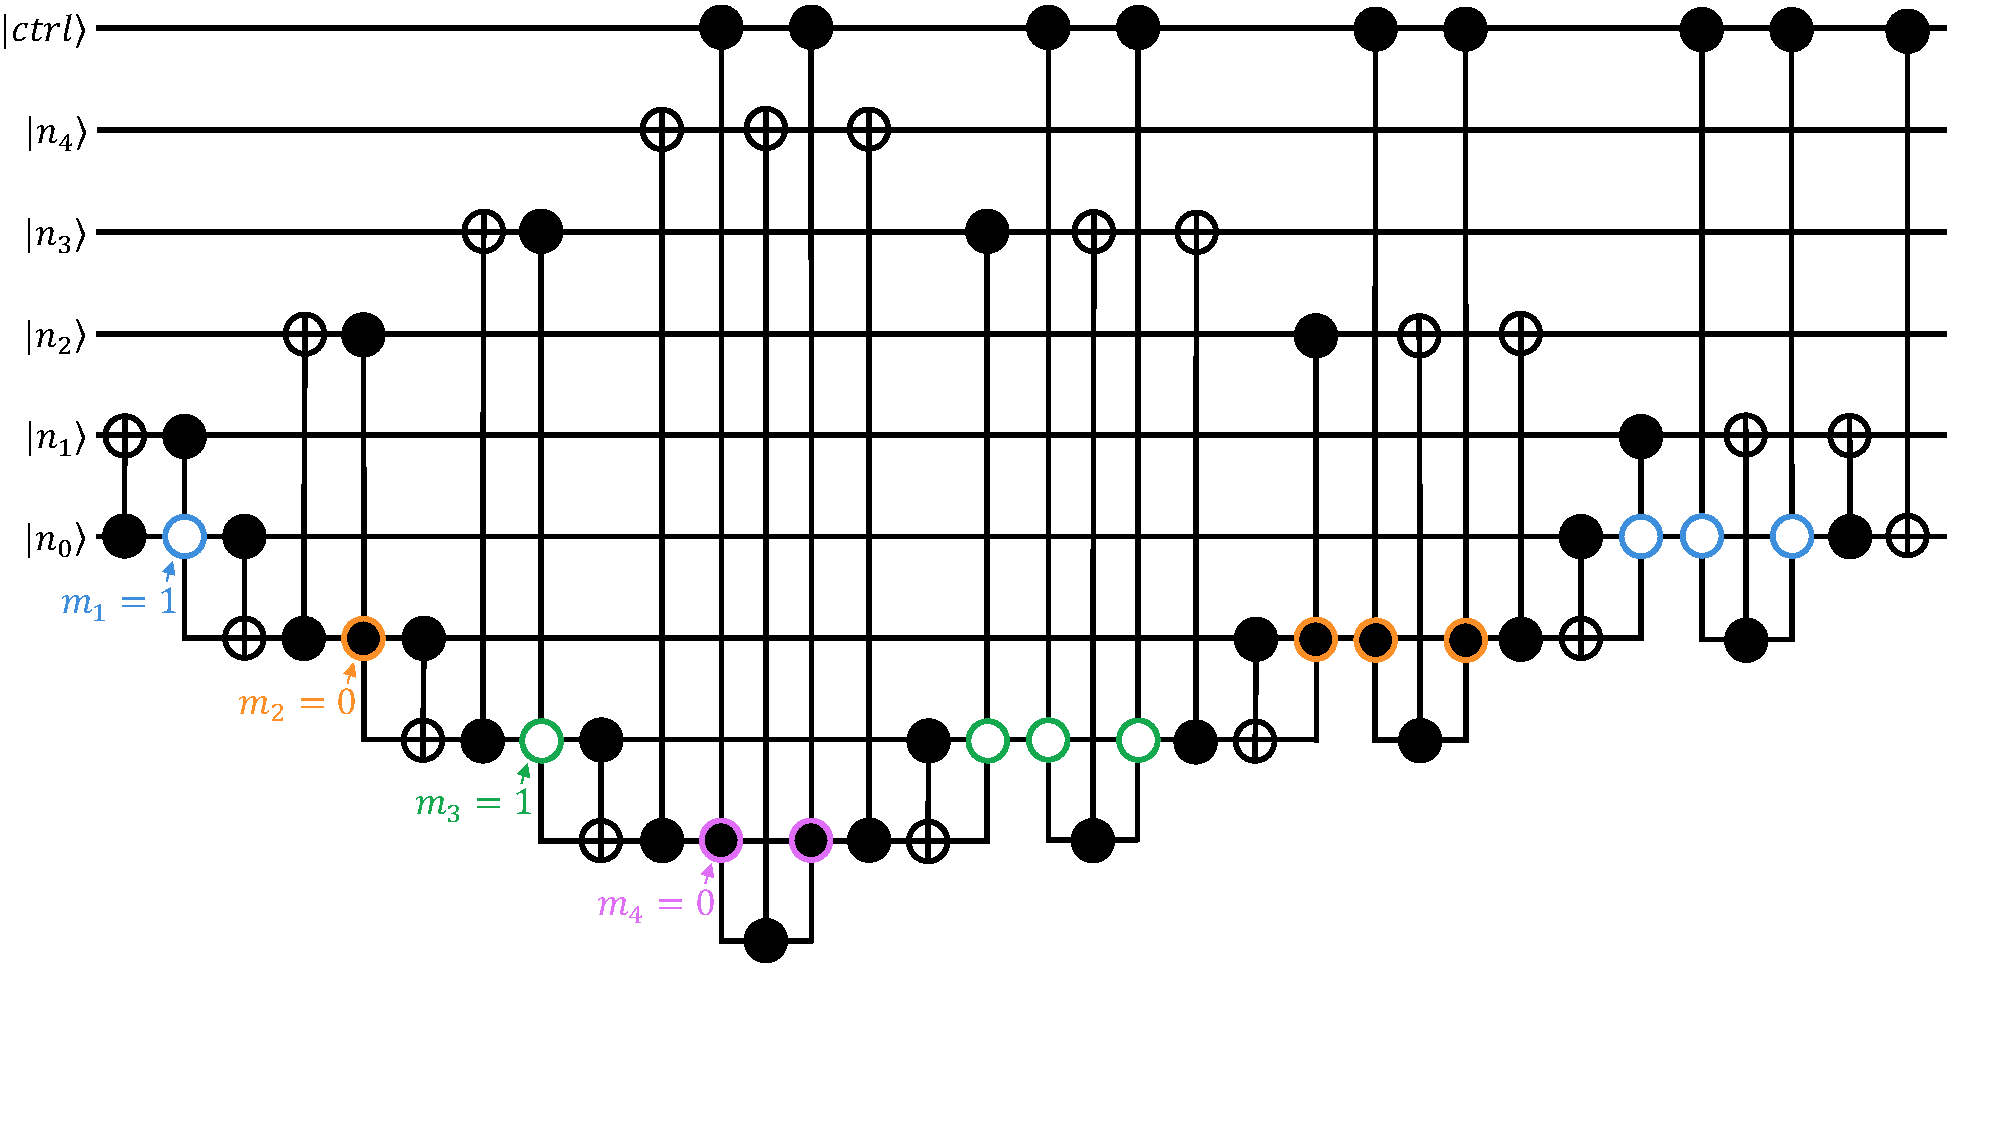
\includegraphics[width=12cm]{figures/ctrl-add-11-qubit-efficient.pdf}
    \caption{
        \textbf{Qubit Efficient Controlled Addition of 11.} 
    }
    \label{fig:addition-qubit-efficient-11}
\end{figure}

\begin{figure}
    \centering
    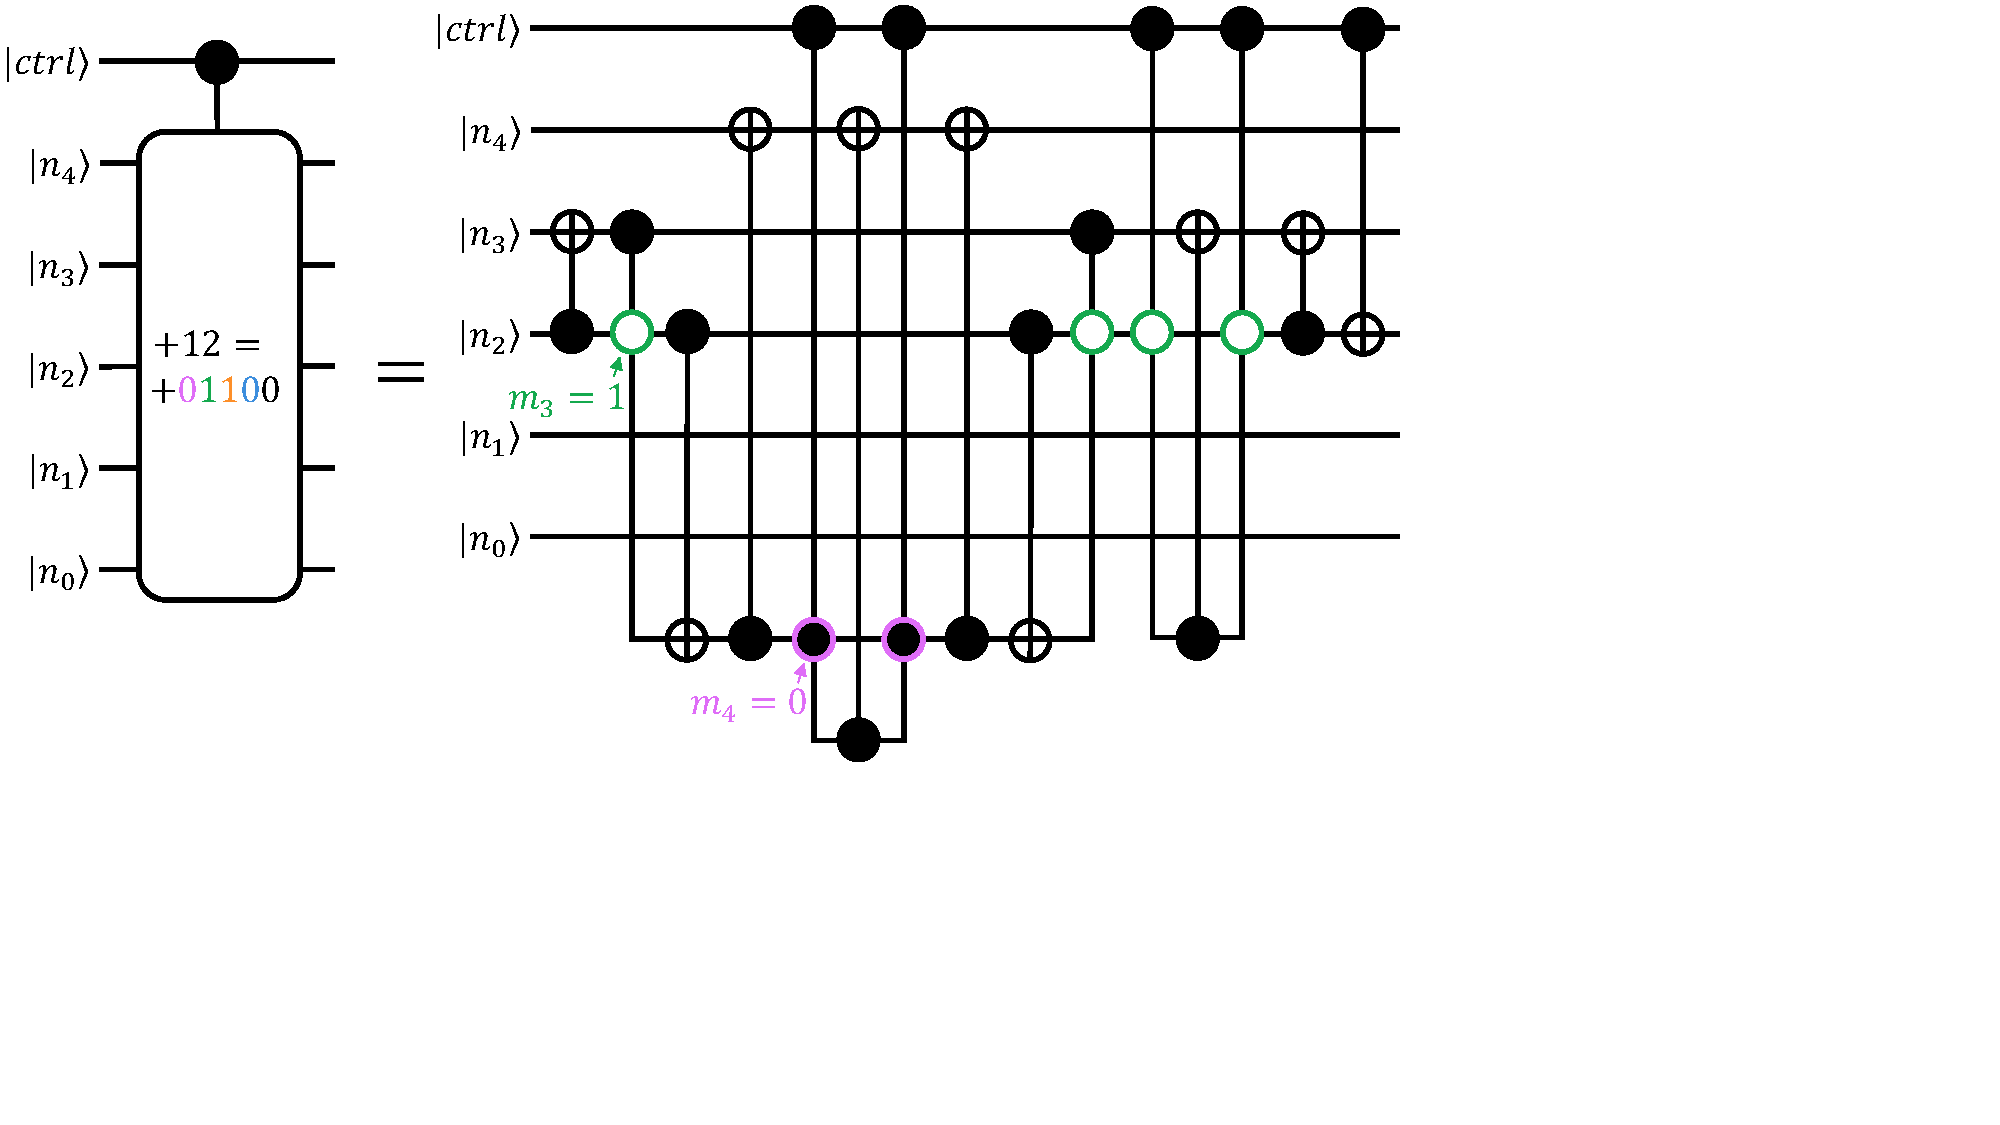
\includegraphics[width=8cm]{figures/ctrl-add-12-qubit-efficient.pdf}
    \caption{
        \textbf{Qubit Efficient Controlled Addition of 12.} 
    }
    \label{fig:addition-qubit-efficient-12}
\end{figure}

Another option is to use the same construction for the controlled quantum adder presented in \cite{gidney2018halving}, but to propagate the controls on the state of $\ket{m}$ into the circuit.
This method removes the register $\ket{m}$ from the quantum circuit, reducing the number of ancillae by $M$.
In Figure \ref{fig:addition-qubit-efficient-11}, we show a decomposition for this circuit when the number being added is $11$ ($01011$ in binary).
Additionally, since the lower bits of $m$ are known, the addition can be performed only beginning on the first non-zero bit of $m$.
An example of performing controlled addition of $12$ ($01100$ in binary) is shown in Figure \ref{fig:addition-qubit-efficient-12} where the $2$ least significant qubits are disregarded.
If the $p$ least significant bits of $m$ are zero, this reduces the cost to $2(N - p) - 3$ left (and right) elbows and $N - p - 1$ ancillae.

\begin{figure}
    \centering
    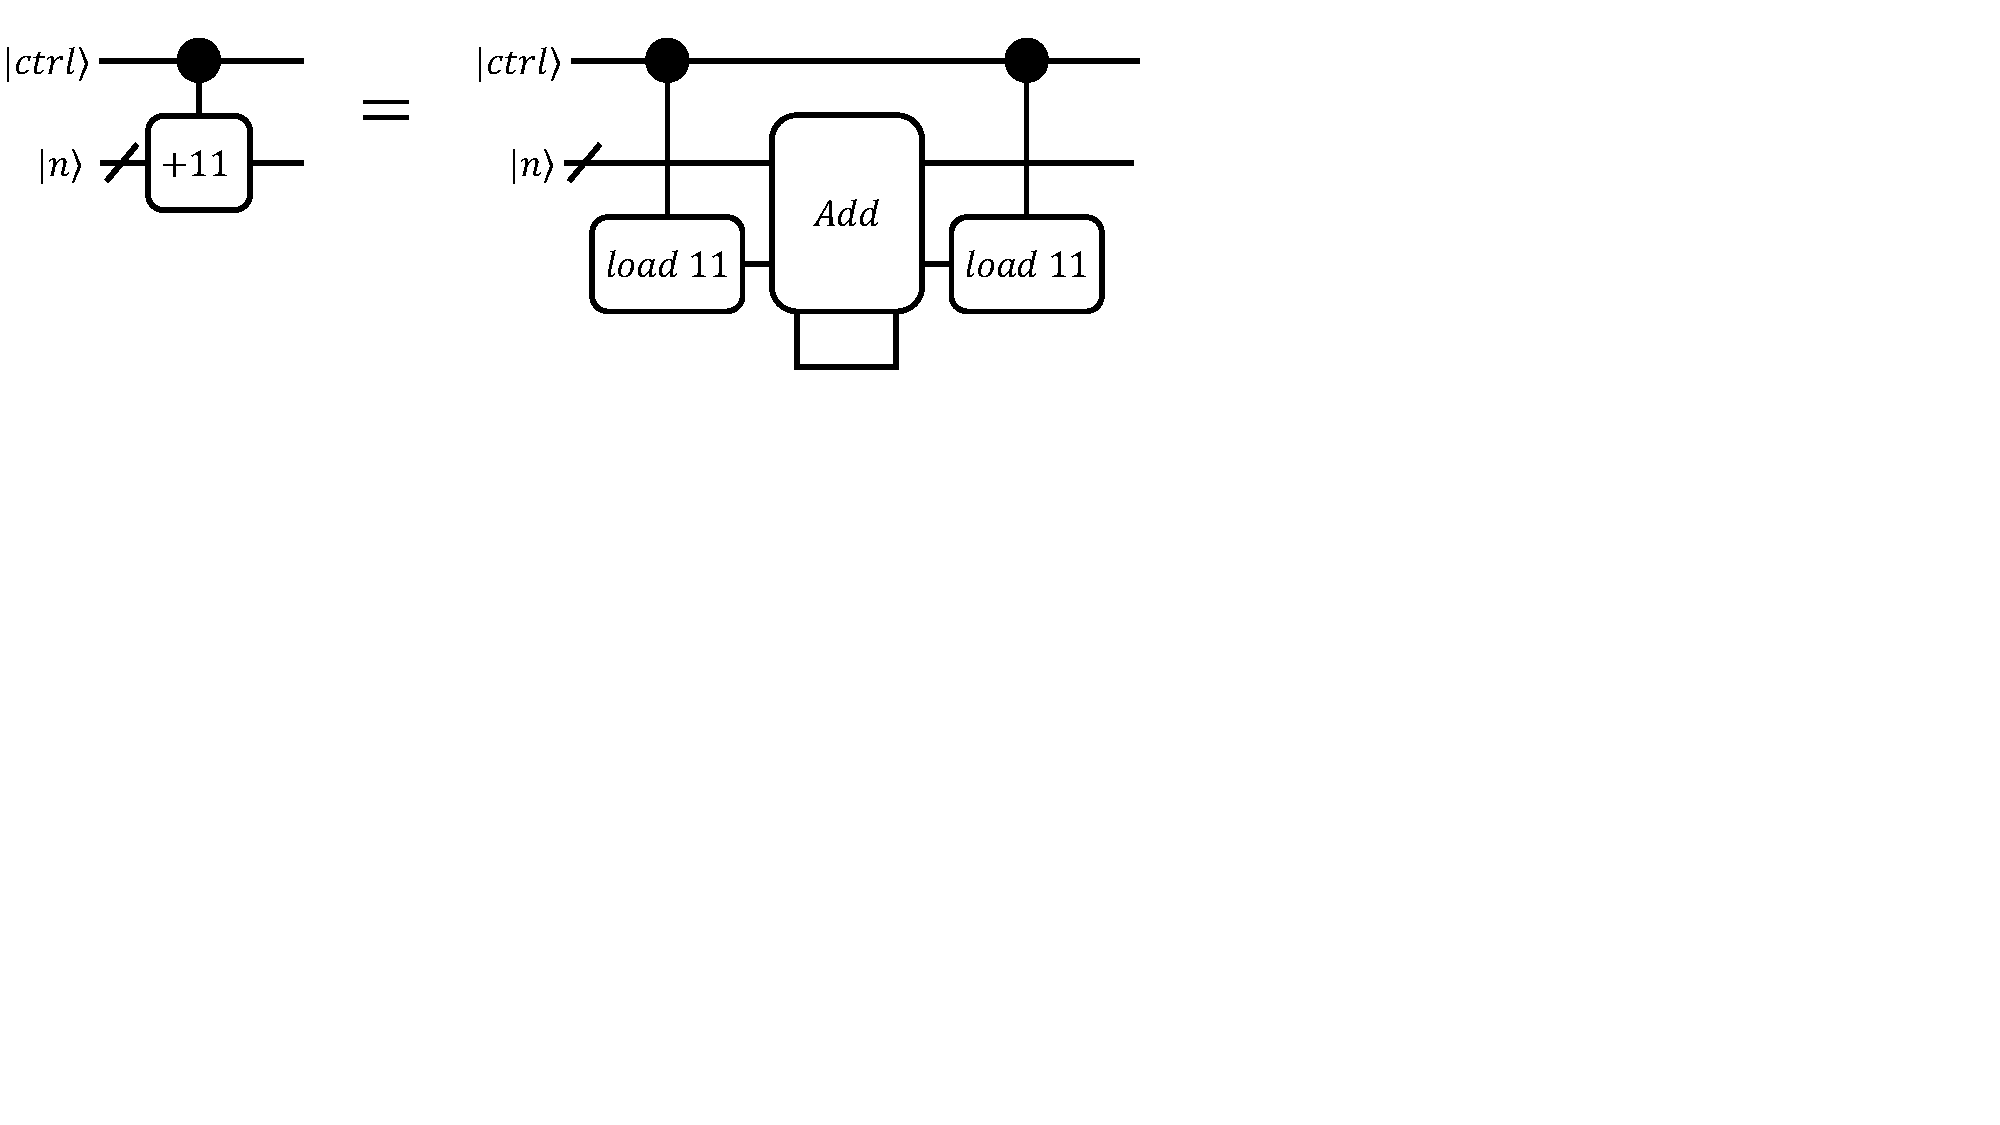
\includegraphics[width=12cm]{figures/ctrl-add-11-gate-efficient.pdf}
    \caption{
        \textbf{Gate Efficient Controlled Quantum Addition.} 
    }
    \label{fig:addition-gate-efficient}
\end{figure}

Lastly, a similar trick using the classical information about $m$ to modify the circuit for controlled addition shown in \cite{gidney2018halving} can reduce the number of left (and right) elbows.
In this construction, the value of $m$ is first loaded into a clean register using a series of CNOTs that are controlled on the control qubit.
The CNOTs present are determine from the binary decomposition of $m$.
Then an uncontrolled addition between the registers $\ket{m}$ and $\ket{n}$ can be performed using the decomposition in \cite{gidney2018halving}.
Finally, the controlled loading of $m$ is then performed again to uncompute the ancillae qubits and return them to a useable state.
A diagram of this ciruit is shown in Figure \ref{fig:addition-gate-efficient}.
Overall, this requires $N - p - 1$ left (and right) elbows and $N + M - p - 1$ ancillae.
Since this option requires the fewest non-Clifford operations while only using a moderate amount of ancillae, this option will be used to determine the resource estimates used in this work.
\section{Uniformly Controlled Rotations}
\label{sec:multiplexed-rotations}

Implementing a series of uniformly controlled rotations is a common subroutine used in this work.
In this section, we discuss the cost and explicit circuit compilation for a series of uniformly controlled rotations around the same axis (but different angles) are applied on the same qubit:
\begin{equation}
    \sum_{l=0}^{L - 1} \ket{l} \ket{\phi} \rightarrow \sum_{l=0}^{L - 1} \ket{l} R_a (\alpha_l) \ket{\phi}
\end{equation}

Möttönen et. al \cite{mottonen2004transformation}, provide a construction for \textit{uncontrolled} uniformly controlled rotations.
This construction is only defined when the number of rotations ($L$) is explicitly a power of $2$, however, if fewer rotations are required, then this can be achieved by padding with zero-angle rotations.

In this construction, the rotation angles are classically preprocessed based on the Gray code (Eq. 3 of \cite{mottonen2004transformation}):
\begin{equation}
    \begin{bmatrix}
        \theta_{0} \\
        \theta_{1} \\
        \vdots \\
        \theta_{L - 1}
    \end{bmatrix} = M \begin{bmatrix}
        \alpha_{0} \\
        \alpha_{1} \\
        \vdots \\
        \alpha_{L - 1}
    \end{bmatrix}
\end{equation}
where $M$ is a matrix transformation defined by:
\begin{equation}
    M_{i, j} = L^{-1} (-1)^{b_{j} . g_{i}}
\end{equation}
where $b_j$ is the binary representation of the integer $j$, $g_i$ is the Gray code representation of the integer $i$, and $b_{j} . g_{i}$ is the bitwise inner product of $b_{j}$ and $g_{i}$.

\begin{figure*}
    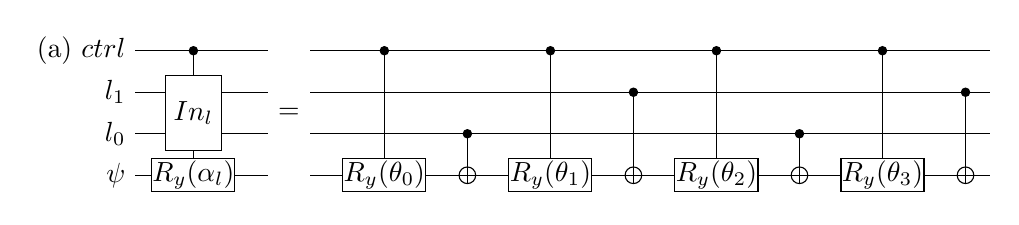
\begin{tikzpicture}[scale=1.000000,x=1pt,y=1pt]
\filldraw[color=white] (0.000000, -7.500000) rectangle (309.000000, 52.500000);
% Drawing wires
% Line 1: ctrl W \text{(a) }ctrl
\draw[color=black] (0.000000,45.000000) -- (309.000000,45.000000);
\draw[color=black] (0.000000,45.000000) node[left] {$\text{(a) }ctrl$};
% Line 2: l1 W l_1
\draw[color=black] (0.000000,30.000000) -- (309.000000,30.000000);
\draw[color=black] (0.000000,30.000000) node[left] {$l_1$};
% Line 3: l0 W l_0
\draw[color=black] (0.000000,15.000000) -- (309.000000,15.000000);
\draw[color=black] (0.000000,15.000000) node[left] {$l_0$};
% Line 4: sys W \psi
\draw[color=black] (0.000000,0.000000) -- (309.000000,0.000000);
\draw[color=black] (0.000000,0.000000) node[left] {$\psi$};
% Done with wires; drawing gates
% Line 6: l1 l0 G:width=20 $In_l$ sys G:width=30 $R_y (\alpha_l)$ ctrl
\draw (21.000000,45.000000) -- (21.000000,0.000000);
\begin{scope}
\draw[fill=white] (21.000000, 22.500000) +(-45.000000:14.142136pt and 19.091883pt) -- +(45.000000:14.142136pt and 19.091883pt) -- +(135.000000:14.142136pt and 19.091883pt) -- +(225.000000:14.142136pt and 19.091883pt) -- cycle;
\clip (21.000000, 22.500000) +(-45.000000:14.142136pt and 19.091883pt) -- +(45.000000:14.142136pt and 19.091883pt) -- +(135.000000:14.142136pt and 19.091883pt) -- +(225.000000:14.142136pt and 19.091883pt) -- cycle;
\draw (21.000000, 22.500000) node {$In_l$};
\end{scope}
\begin{scope}
\draw[fill=white] (21.000000, -0.000000) +(-45.000000:21.213203pt and 8.485281pt) -- +(45.000000:21.213203pt and 8.485281pt) -- +(135.000000:21.213203pt and 8.485281pt) -- +(225.000000:21.213203pt and 8.485281pt) -- cycle;
\clip (21.000000, -0.000000) +(-45.000000:21.213203pt and 8.485281pt) -- +(45.000000:21.213203pt and 8.485281pt) -- +(135.000000:21.213203pt and 8.485281pt) -- +(225.000000:21.213203pt and 8.485281pt) -- cycle;
\draw (21.000000, -0.000000) node {$R_y (\alpha_l)$};
\end{scope}
\filldraw (21.000000, 45.000000) circle(1.500000pt);
% Line 8: =
\draw[fill=white,color=white] (48.000000, -6.000000) rectangle (63.000000, 51.000000);
\draw (55.500000, 22.500000) node {$=$};
% Line 10: sys G width=30 $R_y (\theta_0)$ ctrl
\draw (90.000000,45.000000) -- (90.000000,0.000000);
\begin{scope}
\draw[fill=white] (90.000000, -0.000000) +(-45.000000:21.213203pt and 8.485281pt) -- +(45.000000:21.213203pt and 8.485281pt) -- +(135.000000:21.213203pt and 8.485281pt) -- +(225.000000:21.213203pt and 8.485281pt) -- cycle;
\clip (90.000000, -0.000000) +(-45.000000:21.213203pt and 8.485281pt) -- +(45.000000:21.213203pt and 8.485281pt) -- +(135.000000:21.213203pt and 8.485281pt) -- +(225.000000:21.213203pt and 8.485281pt) -- cycle;
\draw (90.000000, -0.000000) node {$R_y (\theta_0)$};
\end{scope}
\filldraw (90.000000, 45.000000) circle(1.500000pt);
% Line 11: +sys l0
\draw (120.000000,15.000000) -- (120.000000,0.000000);
\begin{scope}
\draw[fill=white] (120.000000, 0.000000) circle(3.000000pt);
\clip (120.000000, 0.000000) circle(3.000000pt);
\draw (117.000000, 0.000000) -- (123.000000, 0.000000);
\draw (120.000000, -3.000000) -- (120.000000, 3.000000);
\end{scope}
\filldraw (120.000000, 15.000000) circle(1.500000pt);
% Line 12: sys G width=30 $R_y (\theta_1)$ ctrl
\draw (150.000000,45.000000) -- (150.000000,0.000000);
\begin{scope}
\draw[fill=white] (150.000000, -0.000000) +(-45.000000:21.213203pt and 8.485281pt) -- +(45.000000:21.213203pt and 8.485281pt) -- +(135.000000:21.213203pt and 8.485281pt) -- +(225.000000:21.213203pt and 8.485281pt) -- cycle;
\clip (150.000000, -0.000000) +(-45.000000:21.213203pt and 8.485281pt) -- +(45.000000:21.213203pt and 8.485281pt) -- +(135.000000:21.213203pt and 8.485281pt) -- +(225.000000:21.213203pt and 8.485281pt) -- cycle;
\draw (150.000000, -0.000000) node {$R_y (\theta_1)$};
\end{scope}
\filldraw (150.000000, 45.000000) circle(1.500000pt);
% Line 13: +sys l1
\draw (180.000000,30.000000) -- (180.000000,0.000000);
\begin{scope}
\draw[fill=white] (180.000000, 0.000000) circle(3.000000pt);
\clip (180.000000, 0.000000) circle(3.000000pt);
\draw (177.000000, 0.000000) -- (183.000000, 0.000000);
\draw (180.000000, -3.000000) -- (180.000000, 3.000000);
\end{scope}
\filldraw (180.000000, 30.000000) circle(1.500000pt);
% Line 14: sys G width=30 $R_y (\theta_2)$ ctrl
\draw (210.000000,45.000000) -- (210.000000,0.000000);
\begin{scope}
\draw[fill=white] (210.000000, -0.000000) +(-45.000000:21.213203pt and 8.485281pt) -- +(45.000000:21.213203pt and 8.485281pt) -- +(135.000000:21.213203pt and 8.485281pt) -- +(225.000000:21.213203pt and 8.485281pt) -- cycle;
\clip (210.000000, -0.000000) +(-45.000000:21.213203pt and 8.485281pt) -- +(45.000000:21.213203pt and 8.485281pt) -- +(135.000000:21.213203pt and 8.485281pt) -- +(225.000000:21.213203pt and 8.485281pt) -- cycle;
\draw (210.000000, -0.000000) node {$R_y (\theta_2)$};
\end{scope}
\filldraw (210.000000, 45.000000) circle(1.500000pt);
% Line 15: +sys l0
\draw (240.000000,15.000000) -- (240.000000,0.000000);
\begin{scope}
\draw[fill=white] (240.000000, 0.000000) circle(3.000000pt);
\clip (240.000000, 0.000000) circle(3.000000pt);
\draw (237.000000, 0.000000) -- (243.000000, 0.000000);
\draw (240.000000, -3.000000) -- (240.000000, 3.000000);
\end{scope}
\filldraw (240.000000, 15.000000) circle(1.500000pt);
% Line 16: sys G width=30 $R_y (\theta_3)$ ctrl
\draw (270.000000,45.000000) -- (270.000000,0.000000);
\begin{scope}
\draw[fill=white] (270.000000, -0.000000) +(-45.000000:21.213203pt and 8.485281pt) -- +(45.000000:21.213203pt and 8.485281pt) -- +(135.000000:21.213203pt and 8.485281pt) -- +(225.000000:21.213203pt and 8.485281pt) -- cycle;
\clip (270.000000, -0.000000) +(-45.000000:21.213203pt and 8.485281pt) -- +(45.000000:21.213203pt and 8.485281pt) -- +(135.000000:21.213203pt and 8.485281pt) -- +(225.000000:21.213203pt and 8.485281pt) -- cycle;
\draw (270.000000, -0.000000) node {$R_y (\theta_3)$};
\end{scope}
\filldraw (270.000000, 45.000000) circle(1.500000pt);
% Line 17: +sys l1
\draw (300.000000,30.000000) -- (300.000000,0.000000);
\begin{scope}
\draw[fill=white] (300.000000, 0.000000) circle(3.000000pt);
\clip (300.000000, 0.000000) circle(3.000000pt);
\draw (297.000000, 0.000000) -- (303.000000, 0.000000);
\draw (300.000000, -3.000000) -- (300.000000, 3.000000);
\end{scope}
\filldraw (300.000000, 30.000000) circle(1.500000pt);
% Done with gates; drawing ending labels
% Done with ending labels; drawing cut lines and comments
% Done with comments
\end{tikzpicture}

    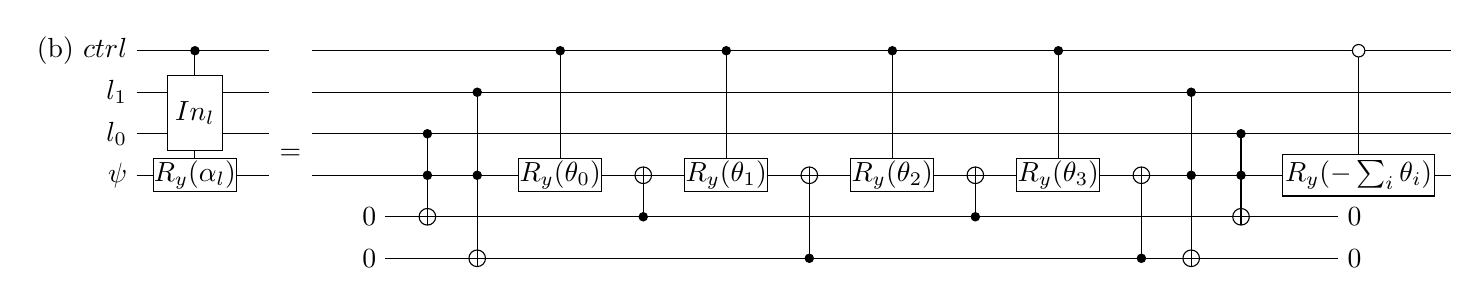
\begin{tikzpicture}[scale=1.000000,x=1pt,y=1pt]
\filldraw[color=white] (0.000000, -7.500000) rectangle (475.000000, 82.500000);
% Drawing wires
% Line 1: ctrl W \text{(b) }ctrl
\draw[color=black] (0.000000,75.000000) -- (475.000000,75.000000);
\draw[color=black] (0.000000,75.000000) node[left] {$\text{(b) }ctrl$};
% Line 2: l1 W l_1
\draw[color=black] (0.000000,60.000000) -- (475.000000,60.000000);
\draw[color=black] (0.000000,60.000000) node[left] {$l_1$};
% Line 3: l0 W l_0
\draw[color=black] (0.000000,45.000000) -- (475.000000,45.000000);
\draw[color=black] (0.000000,45.000000) node[left] {$l_0$};
% Line 4: sys W \psi
\draw[color=black] (0.000000,30.000000) -- (475.000000,30.000000);
\draw[color=black] (0.000000,30.000000) node[left] {$\psi$};
% Line 5: c0 W 0 0
\draw[color=black] (82.500000,15.000000) -- (441.500000,15.000000);
% Line 6: c1 W 0 0
\draw[color=black] (82.500000,0.000000) -- (441.500000,0.000000);
% Done with wires; drawing gates
% Line 8: sys G:width=30 $R_y (\alpha_l)$ l1 l0 G:width=20 $In_l$ ctrl
\draw (21.000000,75.000000) -- (21.000000,30.000000);
\begin{scope}
\draw[fill=white] (21.000000, 30.000000) +(-45.000000:21.213203pt and 8.485281pt) -- +(45.000000:21.213203pt and 8.485281pt) -- +(135.000000:21.213203pt and 8.485281pt) -- +(225.000000:21.213203pt and 8.485281pt) -- cycle;
\clip (21.000000, 30.000000) +(-45.000000:21.213203pt and 8.485281pt) -- +(45.000000:21.213203pt and 8.485281pt) -- +(135.000000:21.213203pt and 8.485281pt) -- +(225.000000:21.213203pt and 8.485281pt) -- cycle;
\draw (21.000000, 30.000000) node {$R_y (\alpha_l)$};
\end{scope}
\begin{scope}
\draw[fill=white] (21.000000, 52.500000) +(-45.000000:14.142136pt and 19.091883pt) -- +(45.000000:14.142136pt and 19.091883pt) -- +(135.000000:14.142136pt and 19.091883pt) -- +(225.000000:14.142136pt and 19.091883pt) -- cycle;
\clip (21.000000, 52.500000) +(-45.000000:14.142136pt and 19.091883pt) -- +(45.000000:14.142136pt and 19.091883pt) -- +(135.000000:14.142136pt and 19.091883pt) -- +(225.000000:14.142136pt and 19.091883pt) -- cycle;
\draw (21.000000, 52.500000) node {$In_l$};
\end{scope}
\filldraw (21.000000, 75.000000) circle(1.500000pt);
% Line 10: =
\draw[fill=white,color=white] (48.000000, -6.000000) rectangle (63.000000, 81.000000);
\draw (55.500000, 37.500000) node {$=$};
% Line 12: c0 c1 START
\draw[color=black] (90.000000,15.000000) node[fill=white,left,minimum height=15.000000pt,minimum width=15.000000pt,inner sep=0pt] {\phantom{$0$}};
\draw[color=black] (90.000000,15.000000) node[left] {$0$};
\draw[color=black] (90.000000,0.000000) node[fill=white,left,minimum height=15.000000pt,minimum width=15.000000pt,inner sep=0pt] {\phantom{$0$}};
\draw[color=black] (90.000000,0.000000) node[left] {$0$};
% Line 13: +c0 sys l0
\draw (105.000000,45.000000) -- (105.000000,15.000000);
\begin{scope}
\draw[fill=white] (105.000000, 15.000000) circle(3.000000pt);
\clip (105.000000, 15.000000) circle(3.000000pt);
\draw (102.000000, 15.000000) -- (108.000000, 15.000000);
\draw (105.000000, 12.000000) -- (105.000000, 18.000000);
\end{scope}
\filldraw (105.000000, 30.000000) circle(1.500000pt);
\filldraw (105.000000, 45.000000) circle(1.500000pt);
% Line 14: +c1 sys l1
\draw (123.000000,60.000000) -- (123.000000,0.000000);
\begin{scope}
\draw[fill=white] (123.000000, 0.000000) circle(3.000000pt);
\clip (123.000000, 0.000000) circle(3.000000pt);
\draw (120.000000, 0.000000) -- (126.000000, 0.000000);
\draw (123.000000, -3.000000) -- (123.000000, 3.000000);
\end{scope}
\filldraw (123.000000, 30.000000) circle(1.500000pt);
\filldraw (123.000000, 60.000000) circle(1.500000pt);
% Line 16: sys G width=30 $R_y (\theta_0)$ ctrl
\draw (153.000000,75.000000) -- (153.000000,30.000000);
\begin{scope}
\draw[fill=white] (153.000000, 30.000000) +(-45.000000:21.213203pt and 8.485281pt) -- +(45.000000:21.213203pt and 8.485281pt) -- +(135.000000:21.213203pt and 8.485281pt) -- +(225.000000:21.213203pt and 8.485281pt) -- cycle;
\clip (153.000000, 30.000000) +(-45.000000:21.213203pt and 8.485281pt) -- +(45.000000:21.213203pt and 8.485281pt) -- +(135.000000:21.213203pt and 8.485281pt) -- +(225.000000:21.213203pt and 8.485281pt) -- cycle;
\draw (153.000000, 30.000000) node {$R_y (\theta_0)$};
\end{scope}
\filldraw (153.000000, 75.000000) circle(1.500000pt);
% Line 17: +sys c0
\draw (183.000000,30.000000) -- (183.000000,15.000000);
\begin{scope}
\draw[fill=white] (183.000000, 30.000000) circle(3.000000pt);
\clip (183.000000, 30.000000) circle(3.000000pt);
\draw (180.000000, 30.000000) -- (186.000000, 30.000000);
\draw (183.000000, 27.000000) -- (183.000000, 33.000000);
\end{scope}
\filldraw (183.000000, 15.000000) circle(1.500000pt);
% Line 18: sys G width=30 $R_y (\theta_1)$ ctrl
\draw (213.000000,75.000000) -- (213.000000,30.000000);
\begin{scope}
\draw[fill=white] (213.000000, 30.000000) +(-45.000000:21.213203pt and 8.485281pt) -- +(45.000000:21.213203pt and 8.485281pt) -- +(135.000000:21.213203pt and 8.485281pt) -- +(225.000000:21.213203pt and 8.485281pt) -- cycle;
\clip (213.000000, 30.000000) +(-45.000000:21.213203pt and 8.485281pt) -- +(45.000000:21.213203pt and 8.485281pt) -- +(135.000000:21.213203pt and 8.485281pt) -- +(225.000000:21.213203pt and 8.485281pt) -- cycle;
\draw (213.000000, 30.000000) node {$R_y (\theta_1)$};
\end{scope}
\filldraw (213.000000, 75.000000) circle(1.500000pt);
% Line 19: +sys c1
\draw (243.000000,30.000000) -- (243.000000,0.000000);
\begin{scope}
\draw[fill=white] (243.000000, 30.000000) circle(3.000000pt);
\clip (243.000000, 30.000000) circle(3.000000pt);
\draw (240.000000, 30.000000) -- (246.000000, 30.000000);
\draw (243.000000, 27.000000) -- (243.000000, 33.000000);
\end{scope}
\filldraw (243.000000, 0.000000) circle(1.500000pt);
% Line 20: sys G width=30 $R_y (\theta_2)$ ctrl
\draw (273.000000,75.000000) -- (273.000000,30.000000);
\begin{scope}
\draw[fill=white] (273.000000, 30.000000) +(-45.000000:21.213203pt and 8.485281pt) -- +(45.000000:21.213203pt and 8.485281pt) -- +(135.000000:21.213203pt and 8.485281pt) -- +(225.000000:21.213203pt and 8.485281pt) -- cycle;
\clip (273.000000, 30.000000) +(-45.000000:21.213203pt and 8.485281pt) -- +(45.000000:21.213203pt and 8.485281pt) -- +(135.000000:21.213203pt and 8.485281pt) -- +(225.000000:21.213203pt and 8.485281pt) -- cycle;
\draw (273.000000, 30.000000) node {$R_y (\theta_2)$};
\end{scope}
\filldraw (273.000000, 75.000000) circle(1.500000pt);
% Line 21: +sys c0
\draw (303.000000,30.000000) -- (303.000000,15.000000);
\begin{scope}
\draw[fill=white] (303.000000, 30.000000) circle(3.000000pt);
\clip (303.000000, 30.000000) circle(3.000000pt);
\draw (300.000000, 30.000000) -- (306.000000, 30.000000);
\draw (303.000000, 27.000000) -- (303.000000, 33.000000);
\end{scope}
\filldraw (303.000000, 15.000000) circle(1.500000pt);
% Line 22: sys G width=30 $R_y (\theta_3)$ ctrl
\draw (333.000000,75.000000) -- (333.000000,30.000000);
\begin{scope}
\draw[fill=white] (333.000000, 30.000000) +(-45.000000:21.213203pt and 8.485281pt) -- +(45.000000:21.213203pt and 8.485281pt) -- +(135.000000:21.213203pt and 8.485281pt) -- +(225.000000:21.213203pt and 8.485281pt) -- cycle;
\clip (333.000000, 30.000000) +(-45.000000:21.213203pt and 8.485281pt) -- +(45.000000:21.213203pt and 8.485281pt) -- +(135.000000:21.213203pt and 8.485281pt) -- +(225.000000:21.213203pt and 8.485281pt) -- cycle;
\draw (333.000000, 30.000000) node {$R_y (\theta_3)$};
\end{scope}
\filldraw (333.000000, 75.000000) circle(1.500000pt);
% Line 23: +sys c1
\draw (363.000000,30.000000) -- (363.000000,0.000000);
\begin{scope}
\draw[fill=white] (363.000000, 30.000000) circle(3.000000pt);
\clip (363.000000, 30.000000) circle(3.000000pt);
\draw (360.000000, 30.000000) -- (366.000000, 30.000000);
\draw (363.000000, 27.000000) -- (363.000000, 33.000000);
\end{scope}
\filldraw (363.000000, 0.000000) circle(1.500000pt);
% Line 25: +c1 sys l1
\draw (381.000000,60.000000) -- (381.000000,0.000000);
\begin{scope}
\draw[fill=white] (381.000000, 0.000000) circle(3.000000pt);
\clip (381.000000, 0.000000) circle(3.000000pt);
\draw (378.000000, 0.000000) -- (384.000000, 0.000000);
\draw (381.000000, -3.000000) -- (381.000000, 3.000000);
\end{scope}
\filldraw (381.000000, 30.000000) circle(1.500000pt);
\filldraw (381.000000, 60.000000) circle(1.500000pt);
% Line 26: +c0 sys l0
\draw (399.000000,45.000000) -- (399.000000,15.000000);
\begin{scope}
\draw[fill=white] (399.000000, 15.000000) circle(3.000000pt);
\clip (399.000000, 15.000000) circle(3.000000pt);
\draw (396.000000, 15.000000) -- (402.000000, 15.000000);
\draw (399.000000, 12.000000) -- (399.000000, 18.000000);
\end{scope}
\filldraw (399.000000, 30.000000) circle(1.500000pt);
\filldraw (399.000000, 45.000000) circle(1.500000pt);
% Line 27: c0 c1 END
\draw[color=black] (434.000000,15.000000) node[fill=white,right,minimum height=15.000000pt,minimum width=15.000000pt,inner sep=0pt] {\phantom{$0$}};
\draw[color=black] (434.000000,15.000000) node[right] {$0$};
\draw[color=black] (434.000000,0.000000) node[fill=white,right,minimum height=15.000000pt,minimum width=15.000000pt,inner sep=0pt] {\phantom{$0$}};
\draw[color=black] (434.000000,0.000000) node[right] {$0$};
% Line 29: sys G:width=55:height=15 $R_y(-\sum_i \theta_i)$ -ctrl
\draw (441.500000,75.000000) -- (441.500000,30.000000);
\begin{scope}
\draw[fill=white] (441.500000, 30.000000) +(-45.000000:38.890873pt and 10.606602pt) -- +(45.000000:38.890873pt and 10.606602pt) -- +(135.000000:38.890873pt and 10.606602pt) -- +(225.000000:38.890873pt and 10.606602pt) -- cycle;
\clip (441.500000, 30.000000) +(-45.000000:38.890873pt and 10.606602pt) -- +(45.000000:38.890873pt and 10.606602pt) -- +(135.000000:38.890873pt and 10.606602pt) -- +(225.000000:38.890873pt and 10.606602pt) -- cycle;
\draw (441.500000, 30.000000) node {$R_y(-\sum_i \theta_i)$};
\end{scope}
\draw[fill=white] (441.500000, 75.000000) circle(2.250000pt);
% Done with gates; drawing ending labels
% Done with ending labels; drawing cut lines and comments
% Done with comments
\end{tikzpicture}

    \caption{
        \textbf{Controlled Uniformly Controlled Rotations}
        Two implementations for controlling a series of uniformly controlled rotations are shown.
        In (a), a naive implementation is shown which doubles the number of arbitrary rotations required.
        The implementation shown in (b) uses only one additional controlled rotation and $\log_2 L$ Toffoli gates, but requires $\log_2 L$ clean ancillae.
    }
    \label{fig:controlled-multiplexed-rotations}
\end{figure*}

However, in this work we require the use of a \textit{controlled} series of uniformly controlled rotations.
Naively, this can be implemented by controlling each of the arbitrary rotations in the construction given by Möttönen et al. \cite{mottonen2004transformation}.
An example circuit diagram for this construction is shown in subfigure \ref{fig:controlled-multiplexed-rotations}a.
Since each controlled rotation can be implemented by two uncontrolled rotations, this compilation strategy uses $2L$ uncontrolled arbitrary rotations.

An alternative approach which uses $4 \log_2 L$ T gates, $L + 3$ arbitrary rotations, and $\log_2 L$ clean ancillae is shown in subfigure \ref{fig:controlled-multiplexed-rotations}b.
In this construction, the temporary logical-AND of each qubit in the index register and the control qubit is computed using $\log_2 L$ Toffoli gates.
CNOTs from these clean ancillae then conjugate each of the arbitrary rotations which are left uncontrolled.
When the control is on, this fully recovers the construction given by Möttönen et. al.

However, when the control is off, the uncontrolled arbitrary rotations are still applied, resulting an undesired rotation of angle $\sum_{i} (\theta_i)$.
This undesired rotation can then be undone using one $0$-controlled rotation of angle $- \sum_{i} (\theta_i)$.

\section{Grover-Rudolph State Preparation}
\label{sec:grover-rudolph}

In this section, we will describe the Grover-Rudolph state-preparation routine \cite{grover2002creating} in the context that it is used in this work.
The Grover-Rudolph state-preparation algorithm constructs quantum circuits that prepare states of the form given by:
\begin{equation}
    \ket{0^{\otimes \lceil \log_2{L} \rceil}} \rightarrow_{\textit{Grover-Rudolph}} \sum_{l=0}^L \sqrt{p(l)} \ket{l}
\end{equation}
where $p(l)$ is a probability distribution along the different indices ($l$) with the constraint that $\sum_l p(l) = 1$.

In the context of block-encodings, preparing such probability distributions can be used to construct the $Prepare$ oracle (Eq. \ref{eq:prep-state}).
The probability distribution in this case is defined by the normalized magnitudes of the coefficients of the terms in the linear combination: $p(l) = |\alpha_l| / \lambda$.

The Grover-Rudolph algorithm works by sequentially summing up the probability distribution to the left and right of a given index and then performing a rotation controlled on the current index.

For example, given the (noramlized) probabilities $\alpha_0$, $\alpha_1$, $\alpha_2$, and $\alpha_3$, the Grover-Rudolph algorithm proceeds as follows:
\begin{enumerate}
    \item Perform a Pauli-Y rotation on the top (left-most) qubit in the register by an angle: $\theta = 2 \cos^{-1}\big( \sqrt{\alpha_0 + \alpha_1} \big)$.
    \item Perform a Pauli-Y rotation on the second qubit in the register, controlled on the first qubit being in the state $\ket{0}$ by an angle: $\theta = 2 \cos^{-1}\big( \sqrt{\frac{\alpha_0}{\alpha_0 + \alpha_1}} \big)$
    \item Perform a Pauli-Y rotation on the second qubit in the register, controlled on the first qubit being in the state $\ket{1}$ by an angle: $\theta = 2 \cos^{-1}\big( \sqrt{\frac{\alpha_2}{\alpha_2 + \alpha_3}} \big)$
\end{enumerate}

The evolution of the quantum state is given by:
\begin{equation}
    \begin{split}
        \ket{00} &\rightarrow_{\textit{(i)}} \sqrt{\alpha_0 + \alpha_1} \ket{00} + \sqrt{\alpha_2 + \alpha_3} \ket{10} \\
        &\rightarrow_{\textit{(ii)}} \sqrt{\alpha_0} \ket{00} + \sqrt{\alpha_1} \ket{01} + \sqrt{\alpha_2 + \alpha_3} \ket{10} \\
        &\rightarrow_{\textit{(iii)}} \sqrt{\alpha_0} \ket{00} + \sqrt{\alpha_1} \ket{01} + \alpha_2 \ket{10} + \alpha_3 \ket{11}
    \end{split}
\end{equation}

\begin{figure*}
    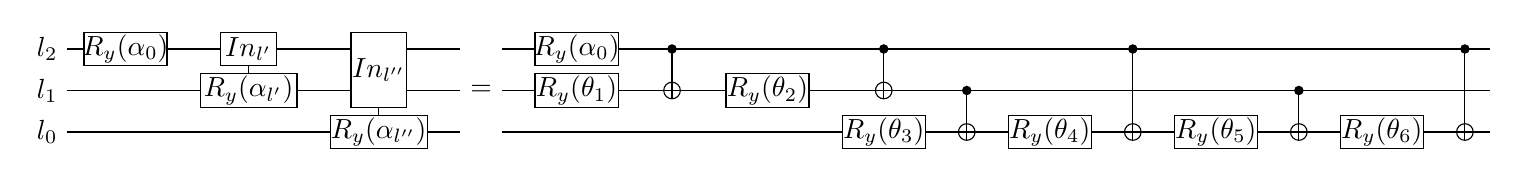
\begin{tikzpicture}[scale=1.000000,x=1pt,y=1pt]
\filldraw[color=white] (0.000000, -7.500000) rectangle (514.000000, 37.500000);
% Drawing wires
% Line 1: l2 W l_2
\draw[color=black] (0.000000,30.000000) -- (514.000000,30.000000);
\draw[color=black] (0.000000,30.000000) node[left] {$l_2$};
% Line 2: l1 W l_1
\draw[color=black] (0.000000,15.000000) -- (514.000000,15.000000);
\draw[color=black] (0.000000,15.000000) node[left] {$l_1$};
% Line 3: l0 W l_0
\draw[color=black] (0.000000,0.000000) -- (514.000000,0.000000);
\draw[color=black] (0.000000,0.000000) node[left] {$l_0$};
% Done with wires; drawing gates
% Line 5: l2 G:width=30 $R_y (\alpha_0)$
\begin{scope}
\draw[fill=white] (21.000000, 30.000000) +(-45.000000:21.213203pt and 8.485281pt) -- +(45.000000:21.213203pt and 8.485281pt) -- +(135.000000:21.213203pt and 8.485281pt) -- +(225.000000:21.213203pt and 8.485281pt) -- cycle;
\clip (21.000000, 30.000000) +(-45.000000:21.213203pt and 8.485281pt) -- +(45.000000:21.213203pt and 8.485281pt) -- +(135.000000:21.213203pt and 8.485281pt) -- +(225.000000:21.213203pt and 8.485281pt) -- cycle;
\draw (21.000000, 30.000000) node {$R_y (\alpha_0)$};
\end{scope}
% Line 6: l1 G:width=35 $R_y (\alpha_{l^\prime})$ l2 G:width=20 $In_{l^\prime}$
\draw (65.500000,30.000000) -- (65.500000,15.000000);
\begin{scope}
\draw[fill=white] (65.500000, 15.000000) +(-45.000000:24.748737pt and 8.485281pt) -- +(45.000000:24.748737pt and 8.485281pt) -- +(135.000000:24.748737pt and 8.485281pt) -- +(225.000000:24.748737pt and 8.485281pt) -- cycle;
\clip (65.500000, 15.000000) +(-45.000000:24.748737pt and 8.485281pt) -- +(45.000000:24.748737pt and 8.485281pt) -- +(135.000000:24.748737pt and 8.485281pt) -- +(225.000000:24.748737pt and 8.485281pt) -- cycle;
\draw (65.500000, 15.000000) node {$R_y (\alpha_{l^\prime})$};
\end{scope}
\begin{scope}
\draw[fill=white] (65.500000, 30.000000) +(-45.000000:14.142136pt and 8.485281pt) -- +(45.000000:14.142136pt and 8.485281pt) -- +(135.000000:14.142136pt and 8.485281pt) -- +(225.000000:14.142136pt and 8.485281pt) -- cycle;
\clip (65.500000, 30.000000) +(-45.000000:14.142136pt and 8.485281pt) -- +(45.000000:14.142136pt and 8.485281pt) -- +(135.000000:14.142136pt and 8.485281pt) -- +(225.000000:14.142136pt and 8.485281pt) -- cycle;
\draw (65.500000, 30.000000) node {$In_{l^\prime}$};
\end{scope}
% Line 7: l0 G:width=35 $R_y (\alpha_{l^{\prime\prime}})$ l2 l1 G:width=20 $In_{l^{\prime\prime}}$
\draw (112.500000,30.000000) -- (112.500000,0.000000);
\begin{scope}
\draw[fill=white] (112.500000, -0.000000) +(-45.000000:24.748737pt and 8.485281pt) -- +(45.000000:24.748737pt and 8.485281pt) -- +(135.000000:24.748737pt and 8.485281pt) -- +(225.000000:24.748737pt and 8.485281pt) -- cycle;
\clip (112.500000, -0.000000) +(-45.000000:24.748737pt and 8.485281pt) -- +(45.000000:24.748737pt and 8.485281pt) -- +(135.000000:24.748737pt and 8.485281pt) -- +(225.000000:24.748737pt and 8.485281pt) -- cycle;
\draw (112.500000, -0.000000) node {$R_y (\alpha_{l^{\prime\prime}})$};
\end{scope}
\begin{scope}
\draw[fill=white] (112.500000, 22.500000) +(-45.000000:14.142136pt and 19.091883pt) -- +(45.000000:14.142136pt and 19.091883pt) -- +(135.000000:14.142136pt and 19.091883pt) -- +(225.000000:14.142136pt and 19.091883pt) -- cycle;
\clip (112.500000, 22.500000) +(-45.000000:14.142136pt and 19.091883pt) -- +(45.000000:14.142136pt and 19.091883pt) -- +(135.000000:14.142136pt and 19.091883pt) -- +(225.000000:14.142136pt and 19.091883pt) -- cycle;
\draw (112.500000, 22.500000) node {$In_{l^{\prime\prime}}$};
\end{scope}
% Line 9: =
\draw[fill=white,color=white] (142.000000, -6.000000) rectangle (157.000000, 36.000000);
\draw (149.500000, 15.000000) node {$=$};
% Line 11: l2 G:width=30 $R_y (\alpha_0)$
\begin{scope}
\draw[fill=white] (184.000000, 30.000000) +(-45.000000:21.213203pt and 8.485281pt) -- +(45.000000:21.213203pt and 8.485281pt) -- +(135.000000:21.213203pt and 8.485281pt) -- +(225.000000:21.213203pt and 8.485281pt) -- cycle;
\clip (184.000000, 30.000000) +(-45.000000:21.213203pt and 8.485281pt) -- +(45.000000:21.213203pt and 8.485281pt) -- +(135.000000:21.213203pt and 8.485281pt) -- +(225.000000:21.213203pt and 8.485281pt) -- cycle;
\draw (184.000000, 30.000000) node {$R_y (\alpha_0)$};
\end{scope}
% Line 13: l1 G:width=30 $R_y (\theta_1)$
\begin{scope}
\draw[fill=white] (184.000000, 15.000000) +(-45.000000:21.213203pt and 8.485281pt) -- +(45.000000:21.213203pt and 8.485281pt) -- +(135.000000:21.213203pt and 8.485281pt) -- +(225.000000:21.213203pt and 8.485281pt) -- cycle;
\clip (184.000000, 15.000000) +(-45.000000:21.213203pt and 8.485281pt) -- +(45.000000:21.213203pt and 8.485281pt) -- +(135.000000:21.213203pt and 8.485281pt) -- +(225.000000:21.213203pt and 8.485281pt) -- cycle;
\draw (184.000000, 15.000000) node {$R_y (\theta_1)$};
\end{scope}
% Line 18: l0 LABEL
% Line 14: l2 +l1
\draw (218.500000,30.000000) -- (218.500000,15.000000);
\filldraw (218.500000, 30.000000) circle(1.500000pt);
\begin{scope}
\draw[fill=white] (218.500000, 15.000000) circle(3.000000pt);
\clip (218.500000, 15.000000) circle(3.000000pt);
\draw (215.500000, 15.000000) -- (221.500000, 15.000000);
\draw (218.500000, 12.000000) -- (218.500000, 18.000000);
\end{scope}
% Line 19: l0 LABEL
% Line 15: l1 G:width=30 $R_y (\theta_2)$
\begin{scope}
\draw[fill=white] (253.000000, 15.000000) +(-45.000000:21.213203pt and 8.485281pt) -- +(45.000000:21.213203pt and 8.485281pt) -- +(135.000000:21.213203pt and 8.485281pt) -- +(225.000000:21.213203pt and 8.485281pt) -- cycle;
\clip (253.000000, 15.000000) +(-45.000000:21.213203pt and 8.485281pt) -- +(45.000000:21.213203pt and 8.485281pt) -- +(135.000000:21.213203pt and 8.485281pt) -- +(225.000000:21.213203pt and 8.485281pt) -- cycle;
\draw (253.000000, 15.000000) node {$R_y (\theta_2)$};
\end{scope}
% Line 20: l0 LABEL
% Line 16: l2 +l1
\draw (295.000000,30.000000) -- (295.000000,15.000000);
\filldraw (295.000000, 30.000000) circle(1.500000pt);
\begin{scope}
\draw[fill=white] (295.000000, 15.000000) circle(3.000000pt);
\clip (295.000000, 15.000000) circle(3.000000pt);
\draw (292.000000, 15.000000) -- (298.000000, 15.000000);
\draw (295.000000, 12.000000) -- (295.000000, 18.000000);
\end{scope}
% Line 21: l0 G:width=30 $R_y (\theta_3)$
\begin{scope}
\draw[fill=white] (295.000000, -0.000000) +(-45.000000:21.213203pt and 8.485281pt) -- +(45.000000:21.213203pt and 8.485281pt) -- +(135.000000:21.213203pt and 8.485281pt) -- +(225.000000:21.213203pt and 8.485281pt) -- cycle;
\clip (295.000000, -0.000000) +(-45.000000:21.213203pt and 8.485281pt) -- +(45.000000:21.213203pt and 8.485281pt) -- +(135.000000:21.213203pt and 8.485281pt) -- +(225.000000:21.213203pt and 8.485281pt) -- cycle;
\draw (295.000000, -0.000000) node {$R_y (\theta_3)$};
\end{scope}
% Line 22: l1 +l0
\draw (325.000000,15.000000) -- (325.000000,0.000000);
\filldraw (325.000000, 15.000000) circle(1.500000pt);
\begin{scope}
\draw[fill=white] (325.000000, 0.000000) circle(3.000000pt);
\clip (325.000000, 0.000000) circle(3.000000pt);
\draw (322.000000, 0.000000) -- (328.000000, 0.000000);
\draw (325.000000, -3.000000) -- (325.000000, 3.000000);
\end{scope}
% Line 23: l0 G:width=30 $R_y (\theta_4)$
\begin{scope}
\draw[fill=white] (355.000000, -0.000000) +(-45.000000:21.213203pt and 8.485281pt) -- +(45.000000:21.213203pt and 8.485281pt) -- +(135.000000:21.213203pt and 8.485281pt) -- +(225.000000:21.213203pt and 8.485281pt) -- cycle;
\clip (355.000000, -0.000000) +(-45.000000:21.213203pt and 8.485281pt) -- +(45.000000:21.213203pt and 8.485281pt) -- +(135.000000:21.213203pt and 8.485281pt) -- +(225.000000:21.213203pt and 8.485281pt) -- cycle;
\draw (355.000000, -0.000000) node {$R_y (\theta_4)$};
\end{scope}
% Line 24: l2 +l0
\draw (385.000000,30.000000) -- (385.000000,0.000000);
\filldraw (385.000000, 30.000000) circle(1.500000pt);
\begin{scope}
\draw[fill=white] (385.000000, 0.000000) circle(3.000000pt);
\clip (385.000000, 0.000000) circle(3.000000pt);
\draw (382.000000, 0.000000) -- (388.000000, 0.000000);
\draw (385.000000, -3.000000) -- (385.000000, 3.000000);
\end{scope}
% Line 25: l0 G:width=30 $R_y (\theta_5)$
\begin{scope}
\draw[fill=white] (415.000000, -0.000000) +(-45.000000:21.213203pt and 8.485281pt) -- +(45.000000:21.213203pt and 8.485281pt) -- +(135.000000:21.213203pt and 8.485281pt) -- +(225.000000:21.213203pt and 8.485281pt) -- cycle;
\clip (415.000000, -0.000000) +(-45.000000:21.213203pt and 8.485281pt) -- +(45.000000:21.213203pt and 8.485281pt) -- +(135.000000:21.213203pt and 8.485281pt) -- +(225.000000:21.213203pt and 8.485281pt) -- cycle;
\draw (415.000000, -0.000000) node {$R_y (\theta_5)$};
\end{scope}
% Line 26: l1 +l0
\draw (445.000000,15.000000) -- (445.000000,0.000000);
\filldraw (445.000000, 15.000000) circle(1.500000pt);
\begin{scope}
\draw[fill=white] (445.000000, 0.000000) circle(3.000000pt);
\clip (445.000000, 0.000000) circle(3.000000pt);
\draw (442.000000, 0.000000) -- (448.000000, 0.000000);
\draw (445.000000, -3.000000) -- (445.000000, 3.000000);
\end{scope}
% Line 27: l0 G:width=30 $R_y (\theta_6)$
\begin{scope}
\draw[fill=white] (475.000000, -0.000000) +(-45.000000:21.213203pt and 8.485281pt) -- +(45.000000:21.213203pt and 8.485281pt) -- +(135.000000:21.213203pt and 8.485281pt) -- +(225.000000:21.213203pt and 8.485281pt) -- cycle;
\clip (475.000000, -0.000000) +(-45.000000:21.213203pt and 8.485281pt) -- +(45.000000:21.213203pt and 8.485281pt) -- +(135.000000:21.213203pt and 8.485281pt) -- +(225.000000:21.213203pt and 8.485281pt) -- cycle;
\draw (475.000000, -0.000000) node {$R_y (\theta_6)$};
\end{scope}
% Line 28: l2 +l0
\draw (505.000000,30.000000) -- (505.000000,0.000000);
\filldraw (505.000000, 30.000000) circle(1.500000pt);
\begin{scope}
\draw[fill=white] (505.000000, 0.000000) circle(3.000000pt);
\clip (505.000000, 0.000000) circle(3.000000pt);
\draw (502.000000, 0.000000) -- (508.000000, 0.000000);
\draw (505.000000, -3.000000) -- (505.000000, 3.000000);
\end{scope}
% Done with gates; drawing ending labels
% Done with ending labels; drawing cut lines and comments
% Done with comments
\end{tikzpicture}

    \caption{
        \textbf{Grover-Rudolph Circuit Compilation.} 
        An implementation of the Grover-Rudolph algorithm using several series of uniformly controlled rotations is shown when $L = 8$.
        This circuit requires $L - 1$ rotations when $L$ is a power of $2$ and the angles of the rotations are changed ($\theta_i \rightarrow \alpha_i$) based on classical preprocessing.
    }
    \label{fig:grover-rudolph}
\end{figure*}


The Grover-Rudolph algorithm can be thought of as performing several series of uniformly controlled rotations.
An example circuit diagram depicting this construction is shown in Figure \ref{fig:grover-rudolph}.
When $L$ is the number of probabilities (or coefficients) to prepare and is a power of $2$, this implementation uses $L-1$ uncontrolled rotations.

\section{Example}
\label{subsec:example}
%Step-by-step example (intention is to move this to an appendix)
Here, a contrived Hamiltonian is used to show the step-by-step procedure of LOBE. The example Hamiltonian, with a bosonic occupancy cutoff $\Omega = 3$, that will be used is 

\begin{equation}
    H = b_0^\dagger d_0(a_0^\dagger)^2 + 2 d_0^\dagger a_0^\dagger a_0+3 b_0^\dagger d_0^\dagger d_0
\end{equation}

\textbf{Step 1: Rescale Hamiltonian from bosonic terms:}
Via equation \ref{bose coeff rescale}, $\frac{1}{(\Omega + 1)^{K/2}} = \frac{1}{4}$ because $K = 2$ (there are at most 2 bosonic creation/annihilation terms, which in this case come from the first term). Now the Hamiltonian becomes 
\begin{equation}
    H^* = \frac{1}{4}H
\end{equation}

\textbf{Step 2: Rescale coefficients of Hamiltonian (assuming USP):} In order to load the Hamiltonian coefficients into the circuit via the $R_y$ gates in the \textit{coefficient} oracle, we need to ensure the coefficients are $\leq 1$. This is done via equation \ref{usp scale}. 
In this case, $L = 3$ since there are three terms, and $\alpha^* = 3$, the largest term coefficient. Thus, $\lambda_{usp} = 12$. Now, via \ref{Hbar scale}, the fully rescaled Hamiltonian is:
\begin{equation}
    \bar{H} = \frac{1}{48}b_0^\dagger d_0(a_0^\dagger)^2 + \frac{1}{24} d_0^\dagger a_0^\dagger a_0+\frac{1}{16} b_0^\dagger d_0^\dagger d_0
\end{equation}

\textbf{Step 3: Obtain the corresponding LOBE circuit:} In the style of figure \ref{fig:select-normal-ordering}, for this particular Hamiltonian, the three \textit{select} oracle unitaries: $U_{T_0}, U_{T_1}, U_{T_2}$ appear as:
\begin{figure}[h]
    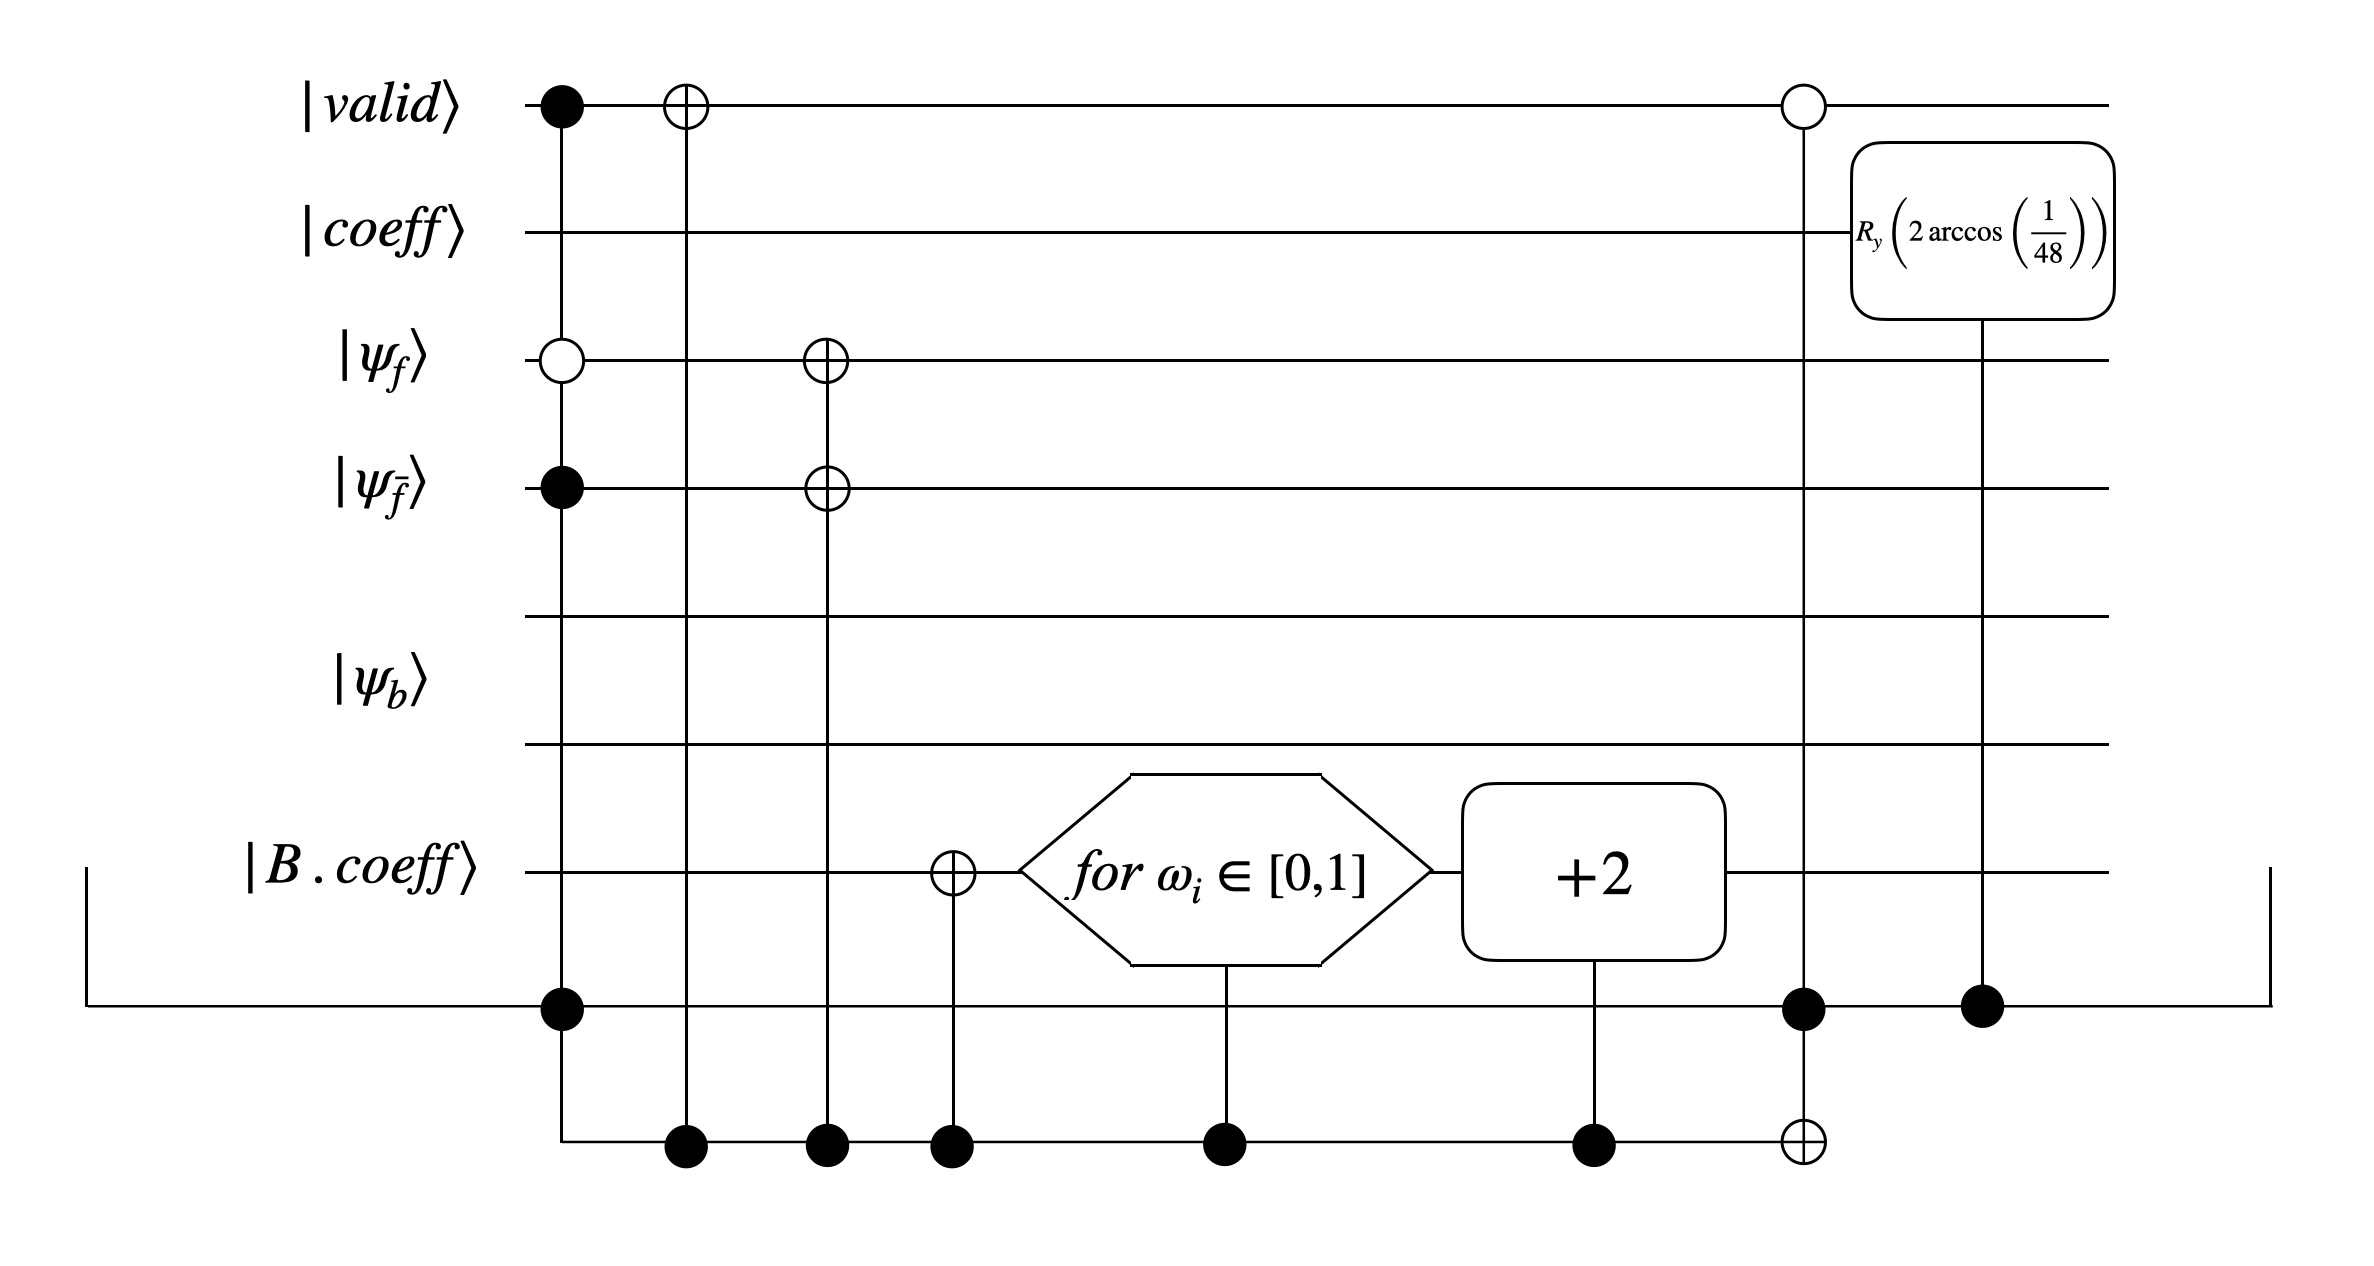
\includegraphics[width = 0.7\linewidth]{figures/T0.png}
    \caption{\textit{Select} unitary $U_{T_0}$ that block-encodes $T_0 = \frac{1}{48}b_0^\dagger d_0(a_0^\dagger)^2$}
\end{figure}
\begin{figure}[h]
    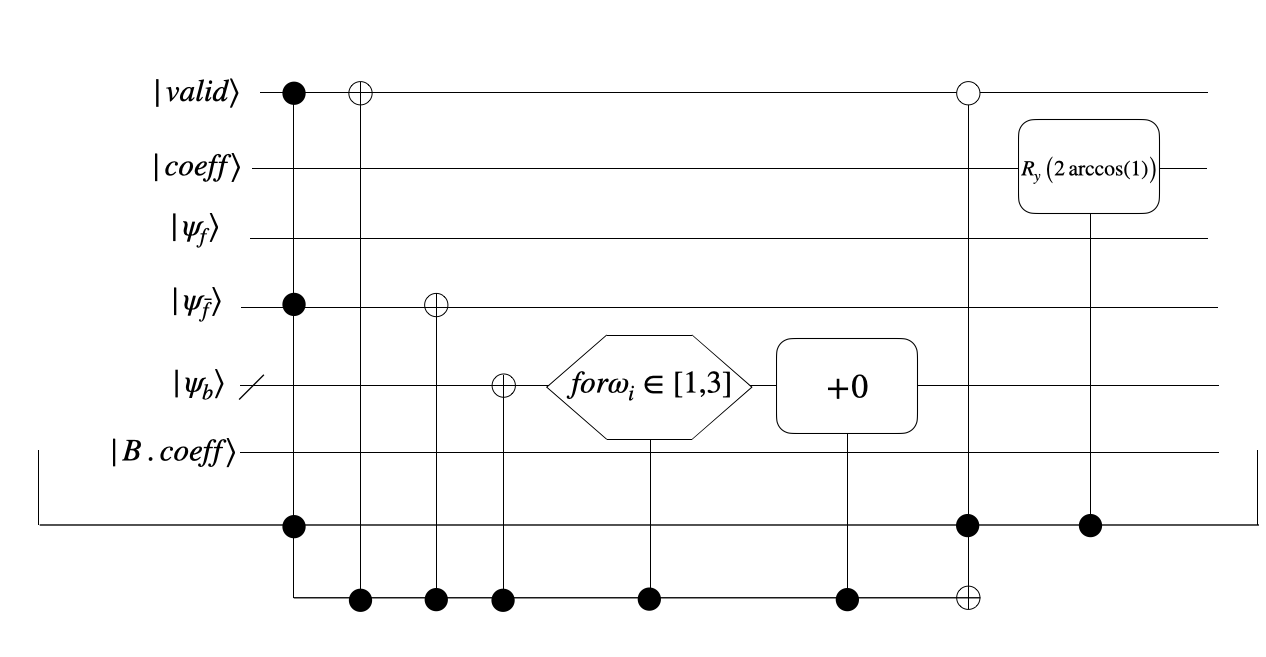
\includegraphics[width = 0.7\linewidth]{figures/T1.png}
    \caption{\textit{Select} unitary $U_{T_1}$ that block-encodes $T_1 = \frac{1}{24}a_0^\dagger a_0 d_0^\dagger$}
\end{figure}
\begin{figure}[h]
    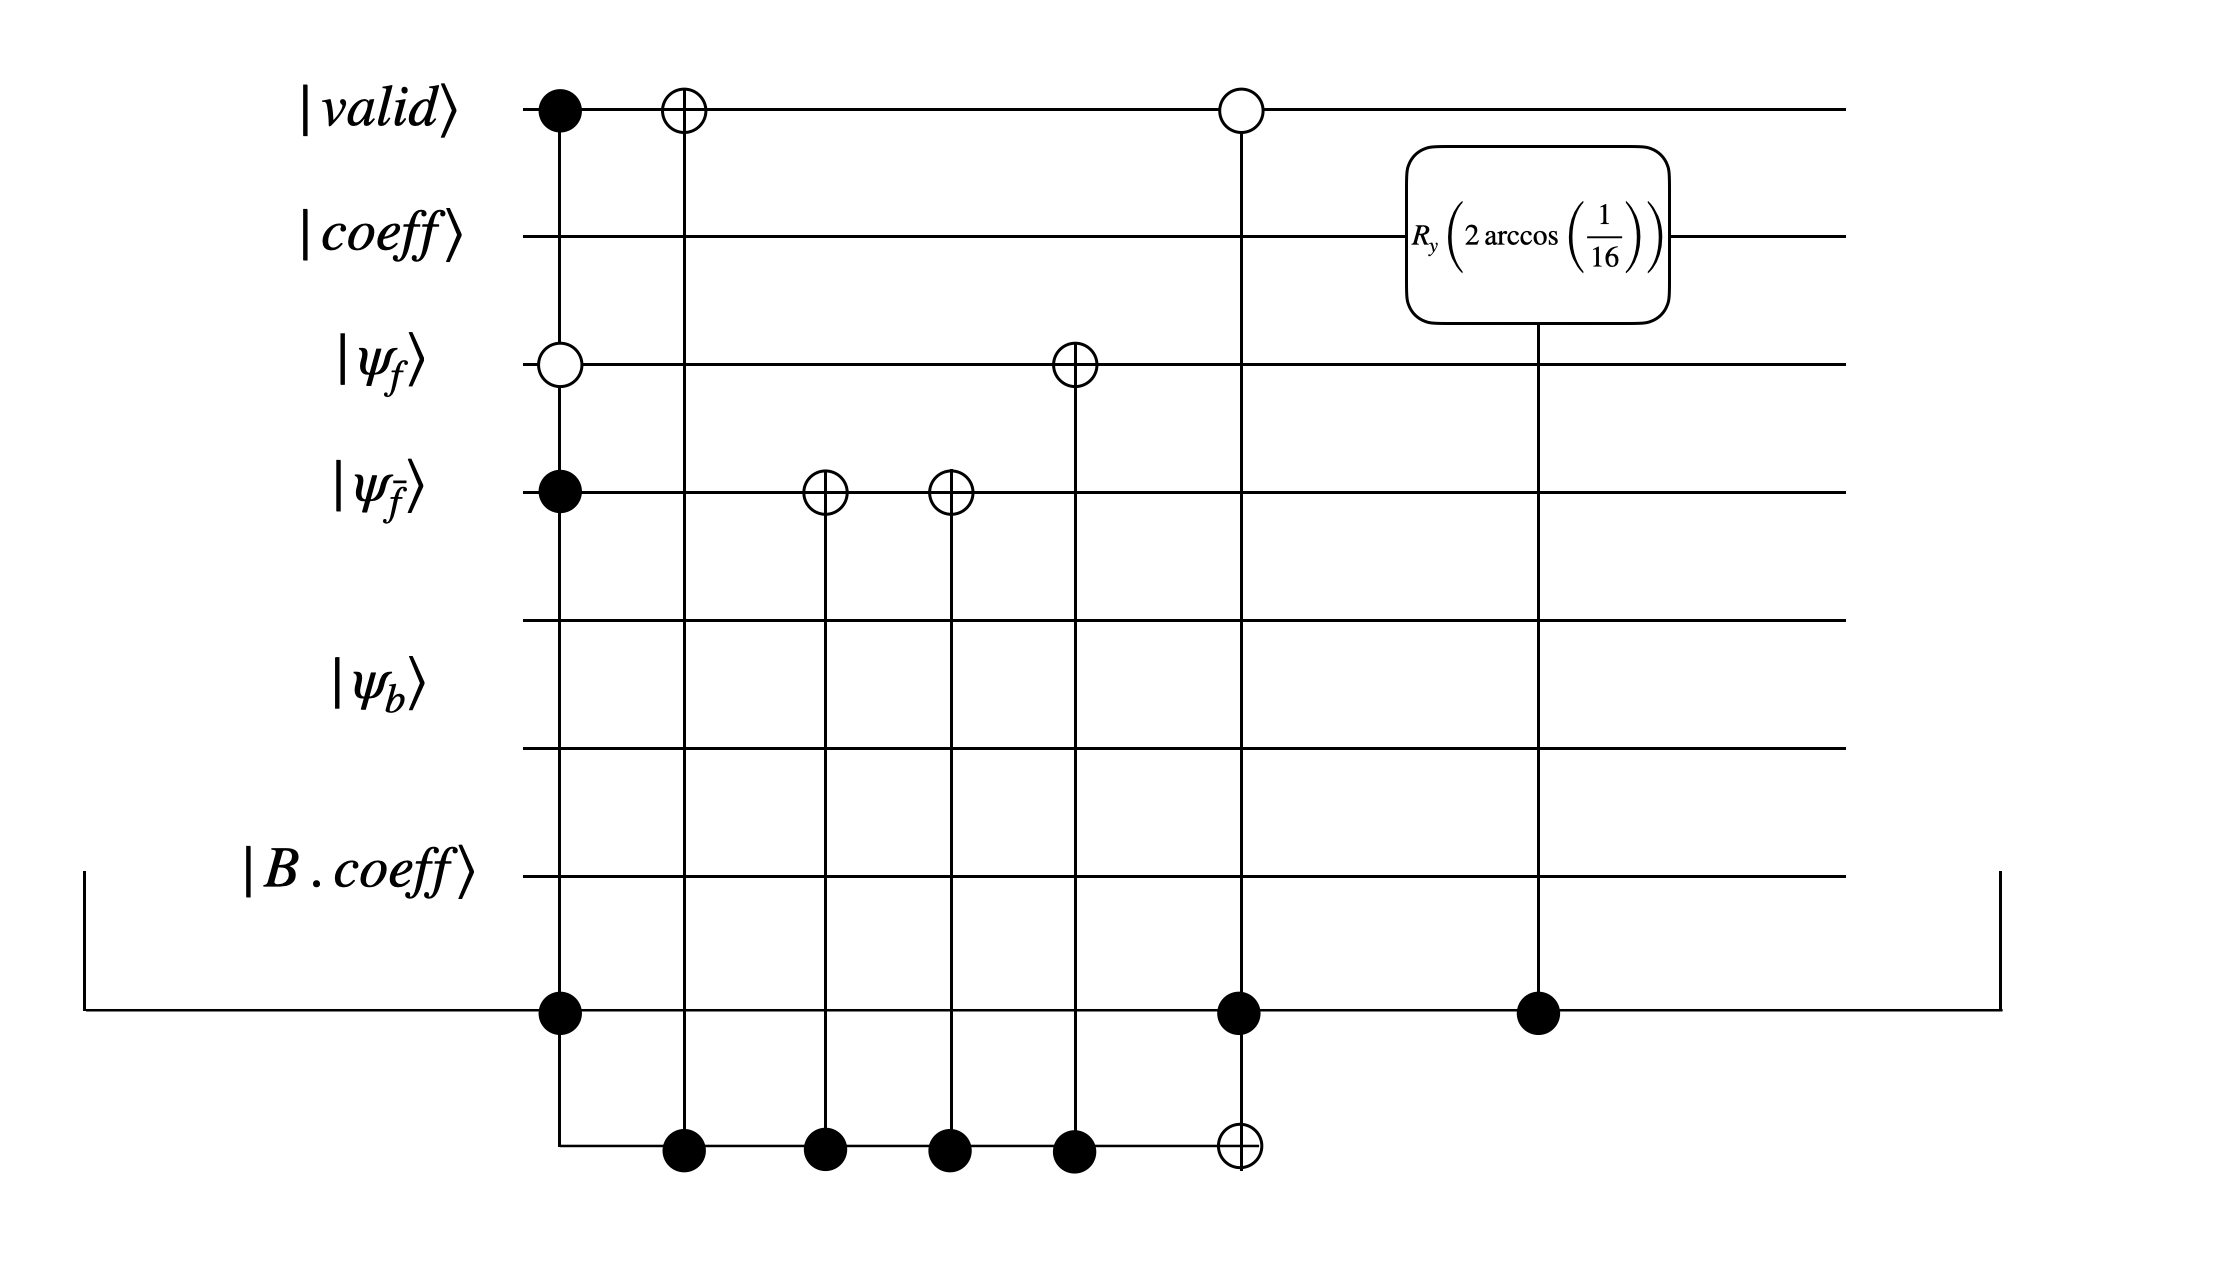
\includegraphics[width = 0.7\linewidth]{figures/T2.png}
    \caption{\textit{Select} unitary $U_{T_2}$ that block-encodes $T_2 = \frac{1}{16}b_0^\dagger d_0^\dagger d_0$}
\end{figure}

\textbf{Step 4: Count gates:} Using the notation in \ref{count gates not.}, the preceeding three unitaries have the following gate counts:

\begin{align}
    C_{U_{T_0}} &= (3, 1, 5, 5)\\
    C_{U_{T_1}} &= (4, 1, 5, 5)\\
    C_{U_{T_2}} &= (1, 1, 3, 3)
\end{align}
Thus, the total cost of the \textit{select} oracle is $C_{\textit{select}} = (8, 3, 13, 13)$. 

\textbf{Step 5: Post-process the eigenvalues:} After obtaining the full block-encoding of the Hamiltonian, the eigenvalues (which can be obtained via phase estimation) must be post-processed. This is because the eigenvalues of the block encoded Hamiltonian will correspond to $\bar{H}$, \textit{not} $H$ (the original problem Hamiltonian).
For this example, $\bar{H} = \frac{1}{48}H$, so if eigenvalues of the block Hamiltonian are obtained as $\bar{E}_i$, then $\bar{E_i} = \frac{1}{48}E_i$. Thus,
\begin{equation}
    E_i = 48\bar{E}_i
\end{equation}
\section{Lightfront Hamiltonians}
\label{subsec:lightfront-hamiltonian}
Here, the explicit discrete form of the Yukawa and $\phi^4$ Hamiltonians will be written out in lightfront coordinates. 

\subsection{Yukawa}
The Hamiltonian is written in terms of fields of discrete momenta, confined to a box, with integration of the Hamiltonian density $\mathcal{H}$ over lightfront space $x^-$:
\begin{align}
    \label{eq:yukawa-hamiltonian-fields}
    H &= H_0 + g\int_{-L}^L dx^- \bar \psi(x) \psi(x) \phi(x)\\ 
    &+ g^2\int_{-L}^L  dx^- \bar \psi(x) \phi(x) \gamma^+\left(i\partial^+ \right)^{-1}\phi(x) \psi(x) \nonumber
\end{align}

The discretized fields are given as:

\begin{align}
    \psi(x) &= \sum_{k = 1/2}^\infty\frac{b_k u(p_k)e^{-ip_k x} + d_k^\dagger v(p_k)e^{ip_k x}}{\sqrt{4\pi k}}\\ 
    \bar \psi(x)&= \sum_{k = 1/2}^\infty\frac{b_k^\dagger \bar u(p_k)e^{ip_k x} + d_k \bar v(p_k)e^{-ip_k x}}{\sqrt{4\pi k}}\\
    \phi(x) &= \sum_{k = 1}^\infty\frac{a_k e^{-ip_k x} + a_k^\dagger e^{ip_k x}}{\sqrt{4\pi k}}
\end{align}

The free part of the Hamiltonian is 

\begin{equation}
    H_0 = \sum_{k = 1/2}^\infty \frac{m_F^2}{p_k^+}\left(b_k^\dagger b_k + d_k^\dagger d_k \right) + \sum_{k = 1}^\infty \frac{m_B^2}{p_k^+}a_k^\dagger a_k 
\end{equation}

Taking a product of the fields and integrating, we get: 
\begin{align*}
    \int_{-L}^L dx^- \bar \psi(x) \psi(x) \phi(x)  = \frac{g(2L)^{5/2}}{(4\pi)^{3/2}} \sum_{k_1, k_2, k_3}^\infty \frac{1}{\sqrt{k_1k_2k_3}}& \left(  b_{k_1}^\dagger b_{k_2}a_{k_3}\bar u(p_{k_1})u(p_{k_2})\delta_{k_1, k_2 + k_3}  \right. \\
      &\left. + b_{k_1}^\dagger b_{k_2}a^\dagger_{k_3}\bar u(p_{k_1})u(p_{k_2})\delta_{k_1 + k_3, k_2} \right)\\
      &\left. + b_{k_1}^\dagger d_{k_2}^\dagger a_{k_3} \bar u(p_{k_1})v(p_{k_2})\delta_{k_1 + k_2, k_3} \right)\\
      &\left. -  b_{k_2}d_{k_1} a^\dagger_{k_3}\bar v(p_{k_1})u(p_{k_2})\delta_{k_3, k_1 + k_2} \right)\\
      &\left. -d_{k_2}^\dagger d_{k_1}  a_{k_3}\bar v(p_{k_1})v(p_{k_2})\delta_{k_2, k_1 + k_3} \right)\\
      &\left. -d_{k_2}^\dagger d_{k_1}  a^\dagger_{k_3}\bar v(p_{k_1})v(p_{k_2})\delta_{k_1, k_2 + k_3} \right)
\end{align*}

where 
\begin{align}
    &\bar u(p_k) u(q_k) = \bar v(p_k) v(q_k) = \sqrt{p_k^+ q_k^+}\left(\frac{m}{p_k^+} + \frac{m}{q_k^+} \right)\\
    &\bar u(p_k) v(q_k) = \bar v(p_k) u(q_k) = \sqrt{p_k^+ q_k^+}\left(\frac{m}{q_k^+} - \frac{m}{p_k^+} \right)
\end{align}

The discretized momentum is given by $p_k = \frac{2\pi k}{L}$

Lastly, the interaction term unique to lightfront coordinates in equation \ref{eq:yukawa-hamiltonian-fields} can be written as:
\begin{align*}
    \int_{-L}^L dx^- \bar \psi(x) \phi(x) \gamma^+ \left(i\partial^+ \right) \phi(x) \psi(x) = \frac{g(2L)^3}{(4\pi)^{2}} \sum_{k_1, k_2, k_3,k_4}^\infty \frac{1}{\sqrt{k_1k_2k_3k_4}}& \left(  b_{k_1}^\dagger b_{k_4}a_{k_2}a_{k_3}\frac{\bar u(p_{k_1})\gamma^+u(p_{k_4})}{p_{k_3} + p_{k_4}}\delta_{k_1, k_2 + k_3 + k_4}  \right. \\
     & \left.-b_{k_1}^\dagger d_{k_4}^\dagger a_{k_2}a_{k_3}\frac{\bar u(p_{k_1})\gamma^+v(p_{k_4})}{p_{k_4} - p_{k_3}}\delta_{k_1 + k_4, k_2 + k_3}\right)  \\
     & \left.-b_{k_1}^\dagger b_{k_4} a_{k_2}a_{k_3}^\dagger \frac{\bar u(p_{k_1})\gamma^+u(p_{k_4})}{p_{k_3} - p_{k_4}}\delta_{k_1 + k_3, k_2 + k_4}\right)  \\
     & \left.-b_{k_1}^\dagger d_{k_4}^\dagger a_{k_2}a_{k_3}^\dagger \frac{\bar u(p_{k_1})\gamma^+v(p_{k_4})}{p_{k_3} + p_{k_4}}\delta_{k_2, k_1 + k_4 + k_3}\right)  \\
     & \left.+b_{k_1}^\dagger b_{k_4} a_{k_2}^\dagger a_{k_3} \frac{\bar u(p_{k_1})\gamma^+u(p_{k_4})}{p_{k_3} + p_{k_4}}\delta_{k_1 + k_2,k_3 + k_4}\right)  \\
     & \left.-b_{k_1}^\dagger d_{k_4}^\dagger a_{k_2}^\dagger a_{k_3} \frac{\bar u(p_{k_1})\gamma^+v(p_{k_4})}{p_{k_4} - p_{k_3}}\delta_{k_3, k_2 + k_1+ k_4}\right)  \\
     & \left.-b_{k_1}^\dagger b_{k_4} a_{k_2}^\dagger a_{k_3}^\dagger \frac{\bar u(p_{k_1})\gamma^+u(p_{k_4})}{p_{k_3} - p_{k_4}}\delta_{k_4, k_2 + k_3 + k_1}\right)  \\
     & \left.+d_{k_4}^\dagger d_{k_1} a_{k_2}a_{k_3} \frac{\bar v(p_{k_1})\gamma^+u(p_{k_4})}{p_{k_4} - p_{k_3}}\delta_{k_4, k_1 + k_2 + k_3}\right)  \\
     & \left. +b_{k_4} d_{k_1} a_{k_2}a_{k_3}^\dagger \frac{\bar v(p_{k_1})\gamma^+v(p_{k_4})}{p_{k_3} - p_{k_4}}\delta_{k_3, k_1 + k_2 + k_4}\right)  \\
     & \left. +d_{k_4}^\dagger d_{k_1} a_{k_2}a_{k_3}^\dagger \frac{\bar v(p_{k_1})\gamma^+u(p_{k_4})}{p_{k_3} + p_{k_4}}\delta_{k_4 + k_3, k_1 + k_2}\right)  \\
     & \left.-b_{k_4} d_{k_1} a_{k_2}^\dagger a_{k_3} \frac{\bar v(p_{k_1})\gamma^+u(p_{k_4})}{p_{k_3} + p_{k_4}}\delta_{k_2, k_4 + k_1 + k_3}\right)  \\
     & \left.+d_{k_4}^\dagger d_{k_1} a_{k_2 }^\dagger a_{k_3}^\dagger \frac{\bar v(p_{k_1})\gamma^+v(p_{k_4})}{p_{k_4} - p_{k_3}}\delta_{k_1, k_2 + k_3 + k_4}\right)  \\
     & \left.-b_{k_4} d_{k_1} a_{k_2}^\dagger a_{k_3}^\dagger \frac{\bar v(p_{k_1})\gamma^+u(p_{k_4})}{p_{k_3} - p_{k_4}}\delta_{k_1 + k_4, k_2 + k_3 }\right)  \\
     & \left.-b_{k_4} d_{k_1} a_{k_2}^\dagger a_{k_3}^\dagger \frac{\bar v(p_{k_1})\gamma^+u(p_{k_4})}{p_{k_3} + p_{k_4}}\delta_{k_1 + k_4, k_2 + k_3}\right)  \\
\end{align*}

where 

\begin{align}
    &\bar u(p_k)\gamma^+ u(q_k) = \bar v(p_k)\gamma^+ v(q_k) = 2\sqrt{p_k^+ q_k^+}\\
    &\bar u(p_k)\gamma^+ v(q_k) = \bar v(p_k)\gamma^+ u(q_k) = -2\sqrt{p_k^+ q_k^+}
\end{align}

\subsection{$\phi^4$}
\gus{Kamil}
\section{Results (Random Operators)}
\label{sec:random-op-results}

In the previous subsections, the costs associated with LOBE are benchmarked for physically relevant models.
In this subsection, we benchmark the same costs for LOBE for randomly generated operators of form of Eq. \ref{eq:lclo}.
\ws{@Gus, we need to describe here how the "random" protocol in OpenParticle works.}

\begin{figure}
    \centering
    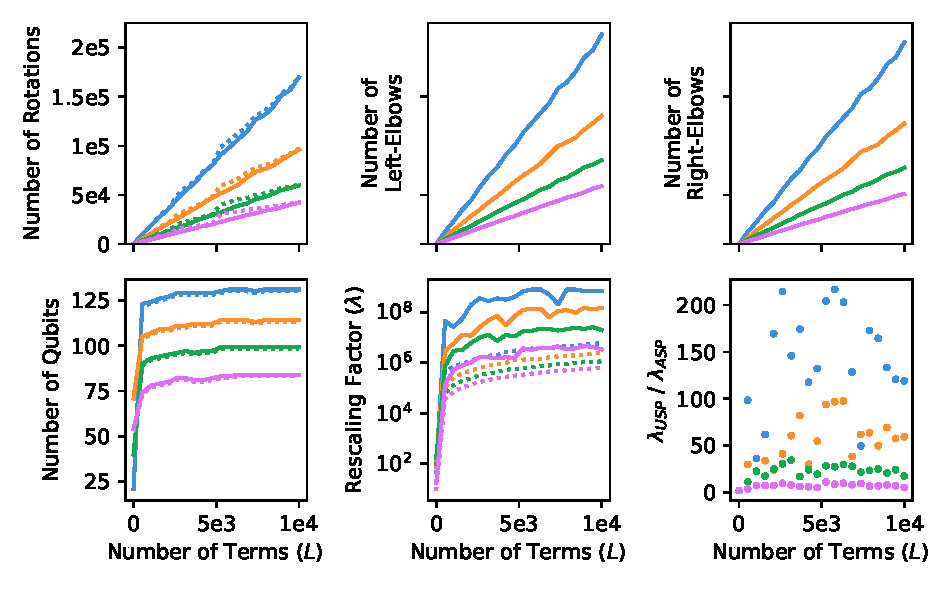
\includegraphics[width=16cm]{figures/random_hamiltonians_metrics_vs_terms.pdf}
    \caption{
        \textbf{Block-Encoding Metrics for Increasing $L$ (Random Hamiltonians).}
        The number of rotations (upper left), left-elbows (upper middle), right-elbows (upper right), number of qubits (lower left), and rescaling factors (lower middle) are plotted as a function of the number of terms in the operator ($L$).
        In the lower right subfigure, the ratio of the two rescaling factors is shown.
        The gate counts for the variant of LOBE using \textit{USP} are shown as the solid lines and those using \textit{ASP} are shown as the dotted lines.
        Metrics for different values of the bosonic occupation cutoff ($\Omega$) are represented in the different colors: $\Omega = 15$ (blue), $\Omega = 7$ (orange), $\Omega = 3$ (green), and $\Omega = 1$ (purple).
        The number of momentum modes ($I$) is set to $15$ and the maximum number of ladder operators per term is set to $5$ ($A_l + B_l + D_l \leq 5$).
        The number of rotations excludes rotations by angles that result in Clifford operations.
    }
    \label{fig:random_hamiltonians_metrics_vs_terms}
\end{figure}

\begin{figure}
    \centering
    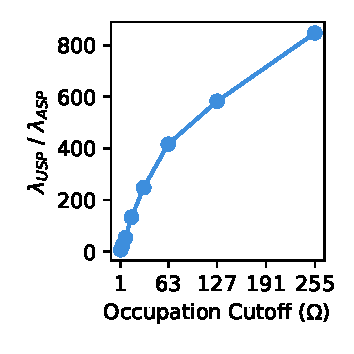
\includegraphics[width=6cm]{figures/random_hamiltonians_rescaling_factor_ratios_vs_omega.pdf}
    \caption{
        \textbf{Ratio of Rescaling Factors for Increasing $\Omega$ (Random Hamiltonians).}
        The average ratio of the two rescaling factors ($\lambda_{USP}$ and $\lambda_{ASP}$) is shown as a function of increasing bosonic occupation cutoff ($\Omega$).
        The number of momentum modes ($I$) is set to $15$ and the maximum number of ladder operators per term ($A + B$) is set to $5$.
        The ratios plotted are the average ratio over 20 unique values of $L$ linearly spaced between $1$ and $10000$.
    }
    \label{fig:random_hamiltonians_rescaling_factor_ratios_vs_omega}
\end{figure}

In Figure \ref{fig:random_hamiltonians_metrics_vs_terms}, we plot the spacetime quantum resources associated with a LOBE block-encoding for randomly generated Hamiltonians.
As is seen for the other models, the number of non-Clifford operations scales linearly with $L$ and the number of qubits scales logarithmically with $L$.
The rescaling factors for both implementations scale logarithmically with $L$.
Additionally, the ratio between the rescaling factors is seemingly independent of $L$, however does appear to increase with $\Omega$.

In Figure \ref{fig:random_hamiltonians_rescaling_factor_ratios_vs_omega}, we plot the average ratio of the rescaling factors for the two variants of LOBE as a function of $\Omega$.
The ratio increases as a function of $\Omega$, indicating that the implementation using \textit{ASP} is increasingly more favorable for models that include a large number of bosons.



\end{document}